%%%%%%%%%%%%%%%%%%%%%%%%%%%%%%%%%%%%%%%%%%%%%%%%%%%
%
%  Author: Jacob Vaughn
%  
%  Last Updated: 3/8/2024
%
%%%%%%%%%%%%%%%%%%%%%%%%%%%%%%%%%%%%%%%%%%%%%%%%%%%

%%%%%%%%%%%%%%%%%%%%%%%%%%%%%%%%%%%%%%%%%%%%%%%%%%%%%%%%%%%%%%%%%%%%%%%
%%%               DESIGN AND FABRICATION OF ACE2.0
%%%%%%%%%%%%%%%%%%%%%%%%%%%%%%%%%%%%%%%%%%%%%%%%%%%%%%%%%%%%%%%%%%%%%%


\chapter{DESIGN AND FABRICATION OF ACE2.0}

\section{Background and Motivation}

As described above, the existing ACE tunnel was designed and manufactured between 2009 and 2010 and began operating in 2010 \cite{ace09,ace10-calibrate,tichenor-dis}. The variable Mach number capability is provided by a thin flexure portion near the end of the nozzle that allows the throat height to be varied from approximately 0.04 to 0.36 inches, which enables the test-section Mach number to be varied from Mach 5 to 8. Schematic of the full tunnel and the nozzle and settling chamber are shown in Figures \ref{fig:ace-full-tunnel} and \ref{fig:ace-nozzle}.

% \textcolor{red}{The ranges of flow conditions are given in Table \ref{tab:flow}.}
% \begin{table}[ht!]
%     \centering
%     \begin{tabular}{ccccc}
%         \hline
%         \hline
%     \textbf{Mach} & \textbf{Total Pressure} & \textbf{Total Temperature} & \textbf{Run Time} & \textbf{Test Section} \\ 
%     \textbf{Number} & \textbf{(psia)} & \textbf{(K)} & \textbf{(sec)} & \textbf{(sq-in.)} \\ \hline
%         5-8 & 30-200 & 300-530 & 50 & 9 $\times$ 14\\ \hline \hline
%     \end{tabular}
%     \caption{ACE operating conditions.}
%     \label{tab:flow}
% \end{table}

\begin{figure}[ht!]
    \centering
    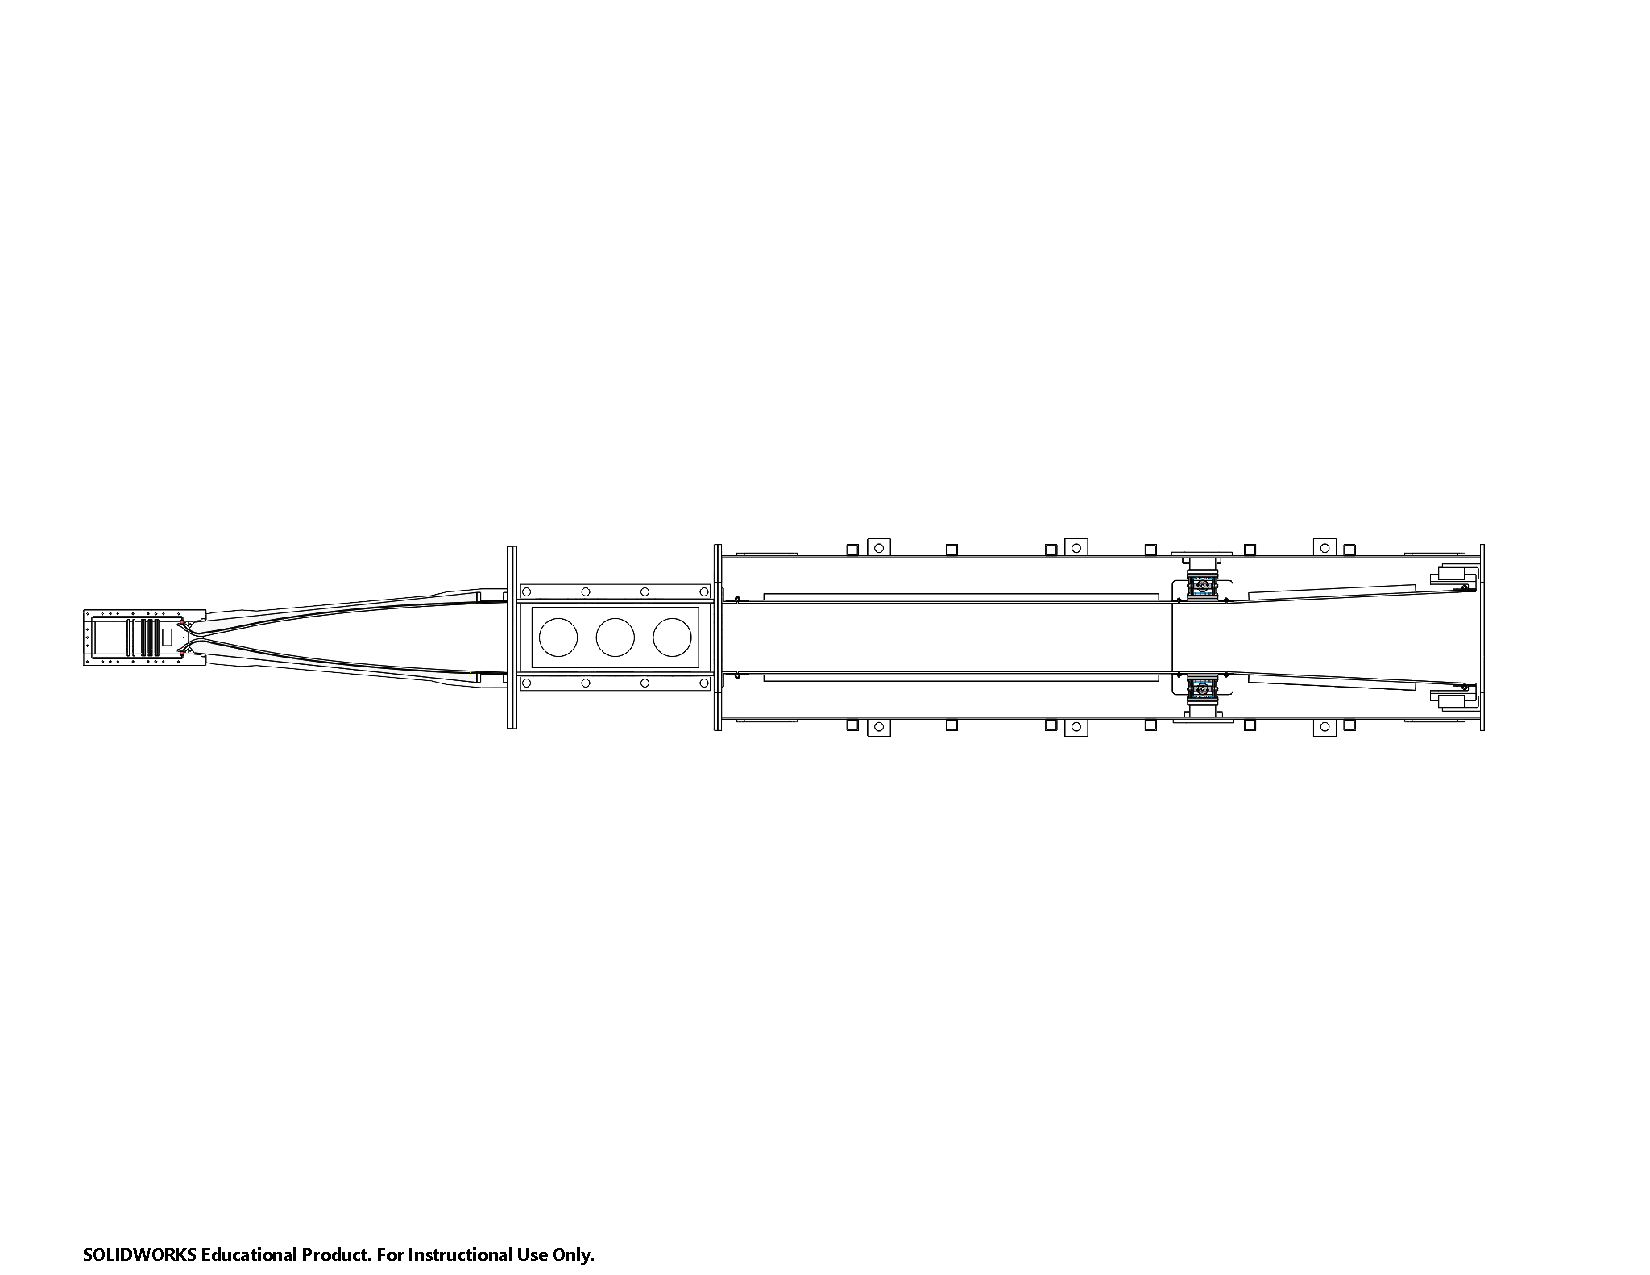
\includegraphics[trim={40 250 60 250},clip,width=6in]{ace-full-tunnel.pdf}
    \caption{ACE tunnel schematic}
    \label{fig:ace-full-tunnel}
\end{figure}

\begin{figure}[ht!]
    \centering
    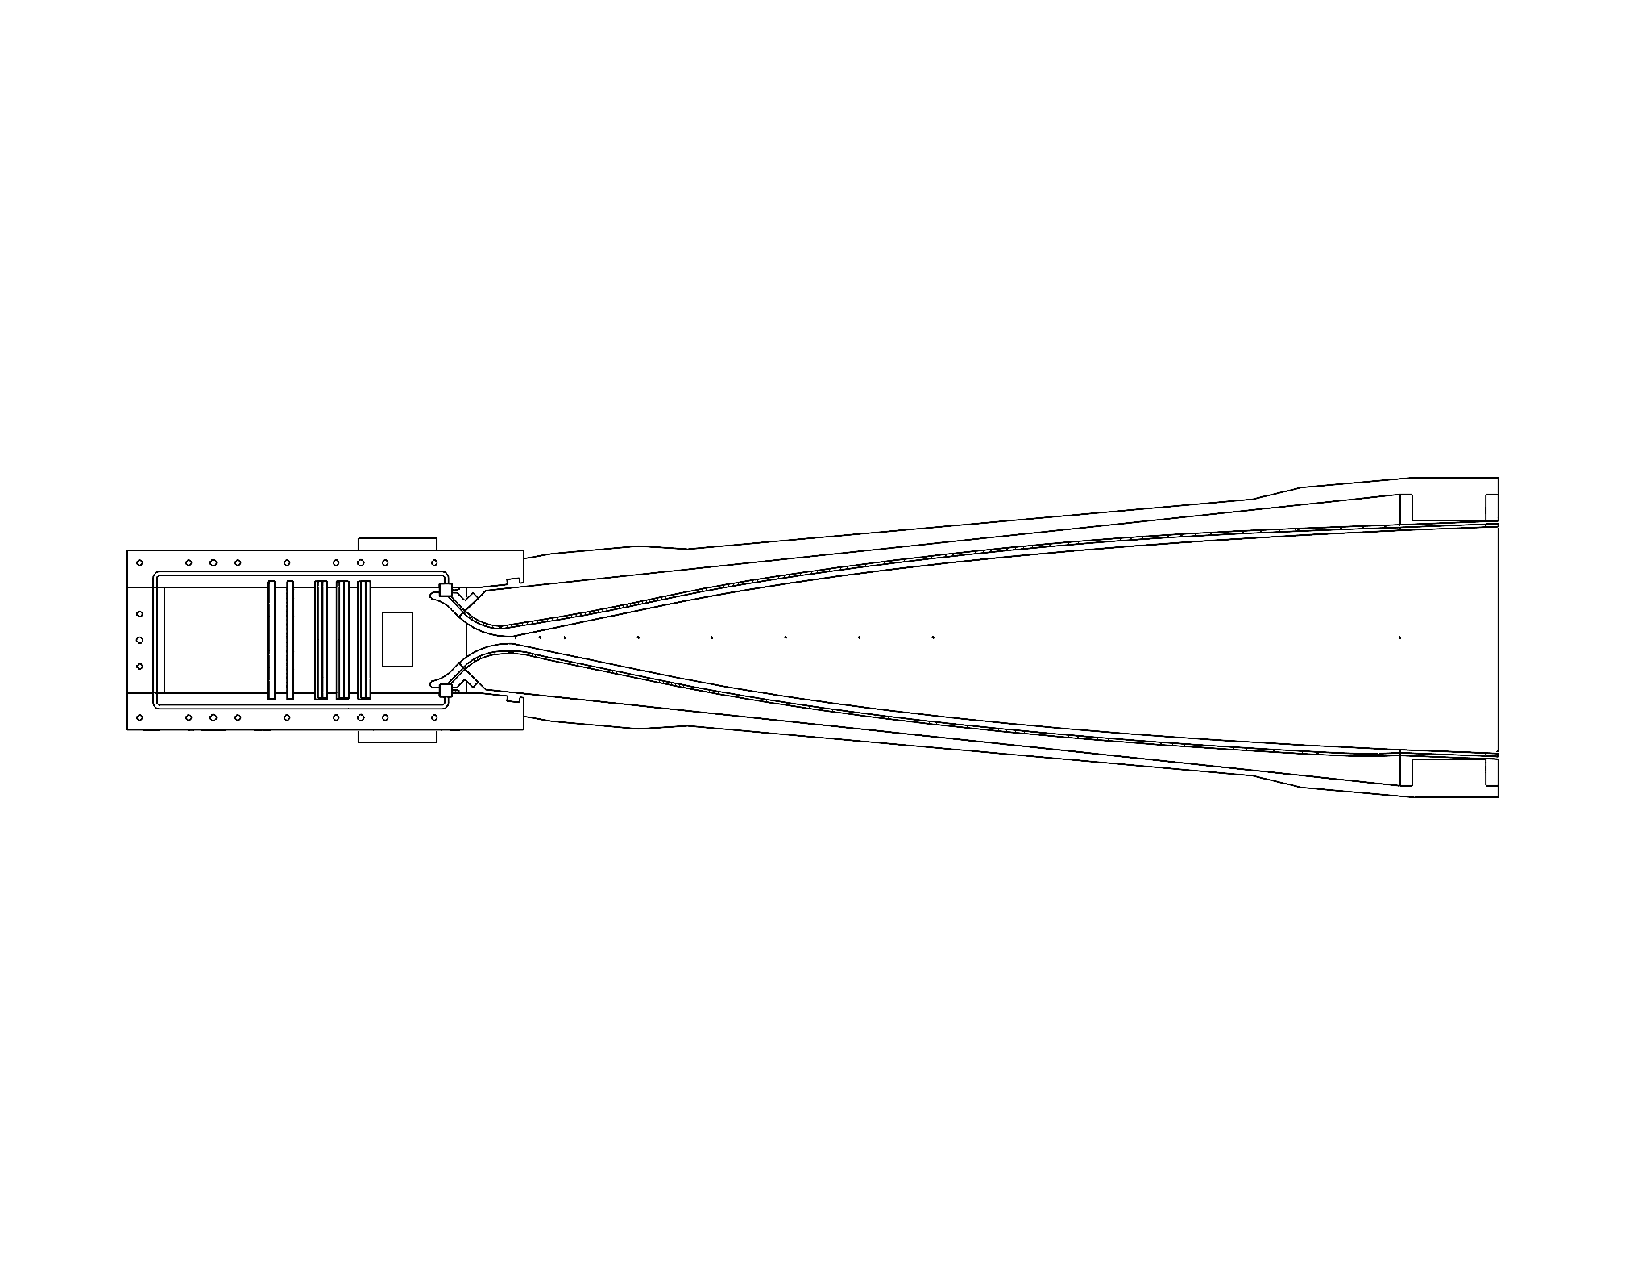
\includegraphics[trim={40 220 40 220},clip,width=6in]{ace-nozzle.pdf}
    \caption{ACE nozzle and settling chamber}
    \label{fig:ace-nozzle}
\end{figure}

The original motivation for the present redesign was to remanufacture the nozzle to remedy the premature laminar-to-turbulent transition, which is discussed in the next section. However, as the work progressed, it became apparent that this redesign was the best opportunity to improve the nozzle and settling chamber to also enable active control. This progression and the redesign process is detailed throughout this chapter.

\subsection{ACE Turbulent Transition}

ACE performance data \cite{aceturb,mai-dis,neel-dis,leidy-dis} shows that below a unit Reynolds number of $Re'$ = $\rho U/\mu \approx 3 \times 10^6/\mathrm{m}$ the RMS pressure fluctuations in the test section are less than 1\%, and that above this unit Reynolds number the pressure fluctuation levels significantly increase. It was desired to increase the unit Reynolds number at which laminar flow can be maintained, so the mechanism causing laminar-to-turbulent transition of the nozzle boundary layers had to be determined. The hypothesis and supporting data regarding the pressure fluctuation levels increase and how it might be delayed to higher unit Reynolds numbers is summarized below.

Five primary suspects for transition were identified:

\begin{enumerate}
    \item A known manufacturing surface discontinuity at the nozzle throat
    \item Sidewall mushroom vortices
    \item Görtler vortices
    \item Freestream turbulence in the incoming flow and/or upstream boundary layer
    \item Wall roughness or waviness
\end{enumerate}

The sections below evaluate each of these possibilities and support the conclusion that the throat discontinuity (1) is the most likely reason for the increased pressure fluctuations above $Re' \approx 3 \times 10^6/\mathrm{m}$. This conclusion is supported by pitot surveys, method-of-characteristics line tracing, and CFD simulations. 

The throat discontinuity is the result of a decimal truncation error of about 0.0003 inches at the interface connecting the subsonic curve to the supersonic MOC contour in the original design files. The resulting discontinuity is shown in Figure \ref{fig:ace-throat}. The artifact carried forward through the CNC machining and is present on the physical nozzle throat.

\begin{figure}[ht!]
    \centering
    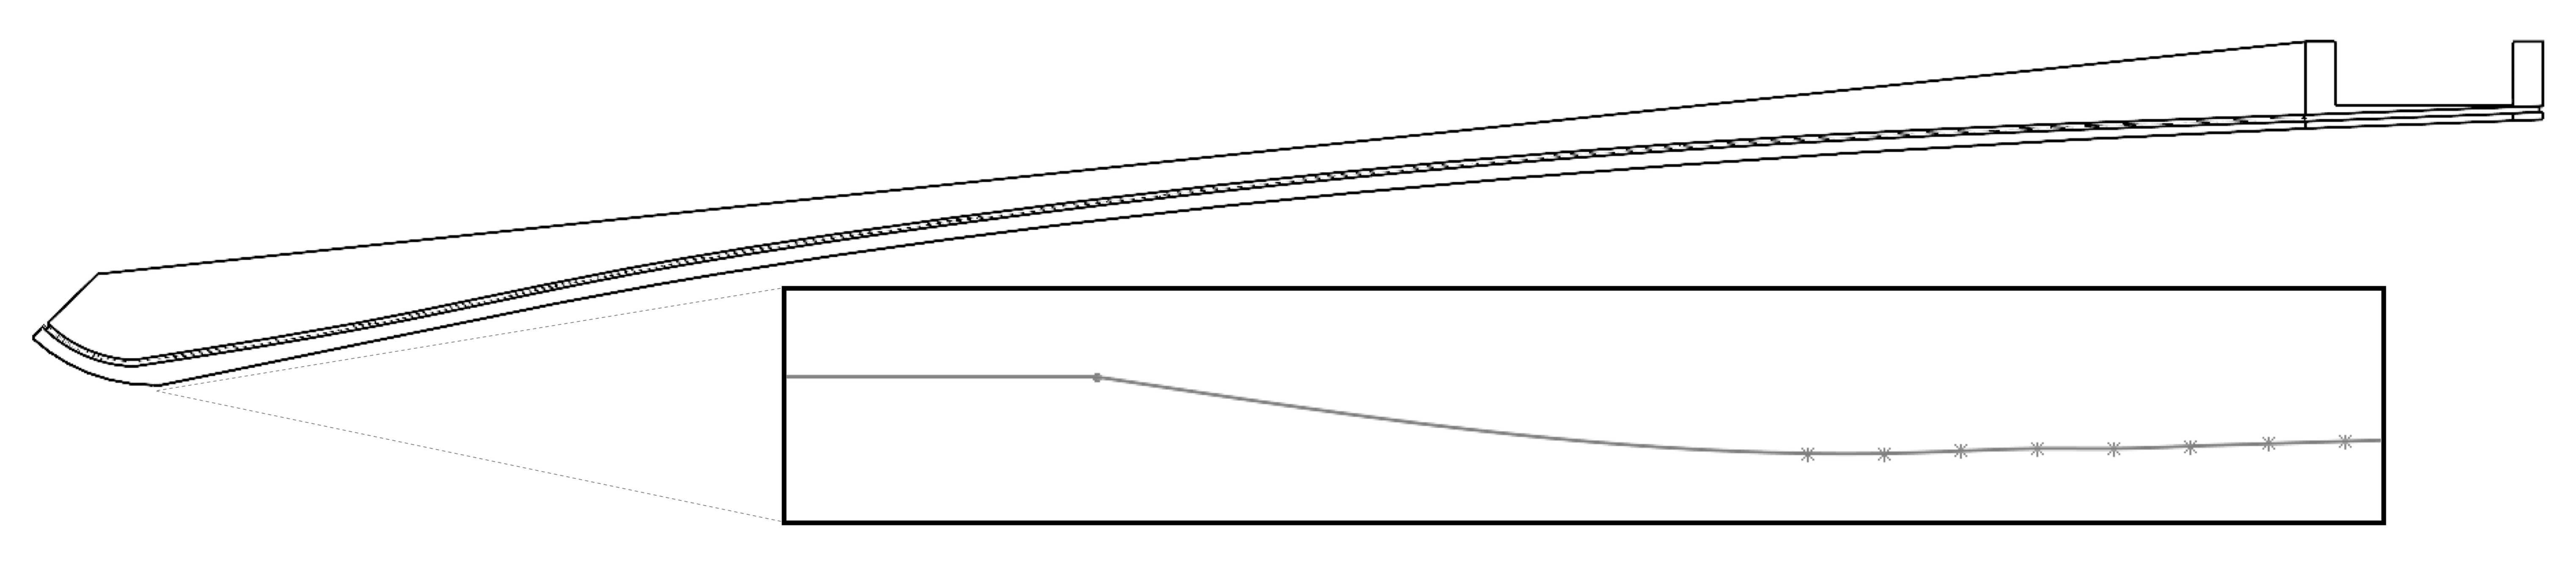
\includegraphics[width=6in]{ace-throat}
    \caption{ACE throat discontinuity}
    \label{fig:ace-throat}
\end{figure}


Sidewall mushroom vortices (2) and Görtler vortices (3) would lead to transition too far downstream from the throat to be responsible for the pressure fluctuation levels increase. Incoming freestream turbulence (4) and wall surface quality (5) are potential causes of poor flow quality in all supersonic tunnels and are included for completeness. The specific mechanism by which these would cause transition is not known. While item 4 and 5 are not the primary suspects for the pressure fluctuation levels increase, improving these conditions will be addressed in the redesign intended to extend laminar flow to higher unit Reynolds numbers.

\subsubsection*{ACE Nozzle Noise Surveys}

Three recent pitot surveys have been conducted in the ACE tunnel. The first by Mai in 2014 \cite{mai-dis} revealed transition occurring around $Re' \approx 3 \times 10^6/\mathrm{m}$, as shown in Figure \ref{fig:mai-survey}. The same result was found by Neel in 2019 \cite{neel-dis} shown in Figure \ref{fig:neel-survey} that transition occurs at this $Re'$ value at a location 6 inches upstream of the nozzle exit. As part of this work, a final pitot survey in ACE was conducted to determine whether the pressure fluctuation levels increase occurred at different $Re'$ values at positions farther upstream in the nozzle. It was found that pressure fluctuation levels increase at the same $Re' \approx 3 \times 10^6/\mathrm{m}$ at a measurement location 24 inches upstream of the nozzle exit. These results in Figure \ref{fig:ace-survey-2024} align with Mai's and Neel's data and clearly establish that the Reynolds number at which pressure fluctuation levels increase is the same at all locations in the nozzle. This suggests that transition is not moving upstream through the nozzle as Reynolds number is increased, as might be expected for typical boundary-layer instability processes.

\begin{figure}[ht!]
    \centering
    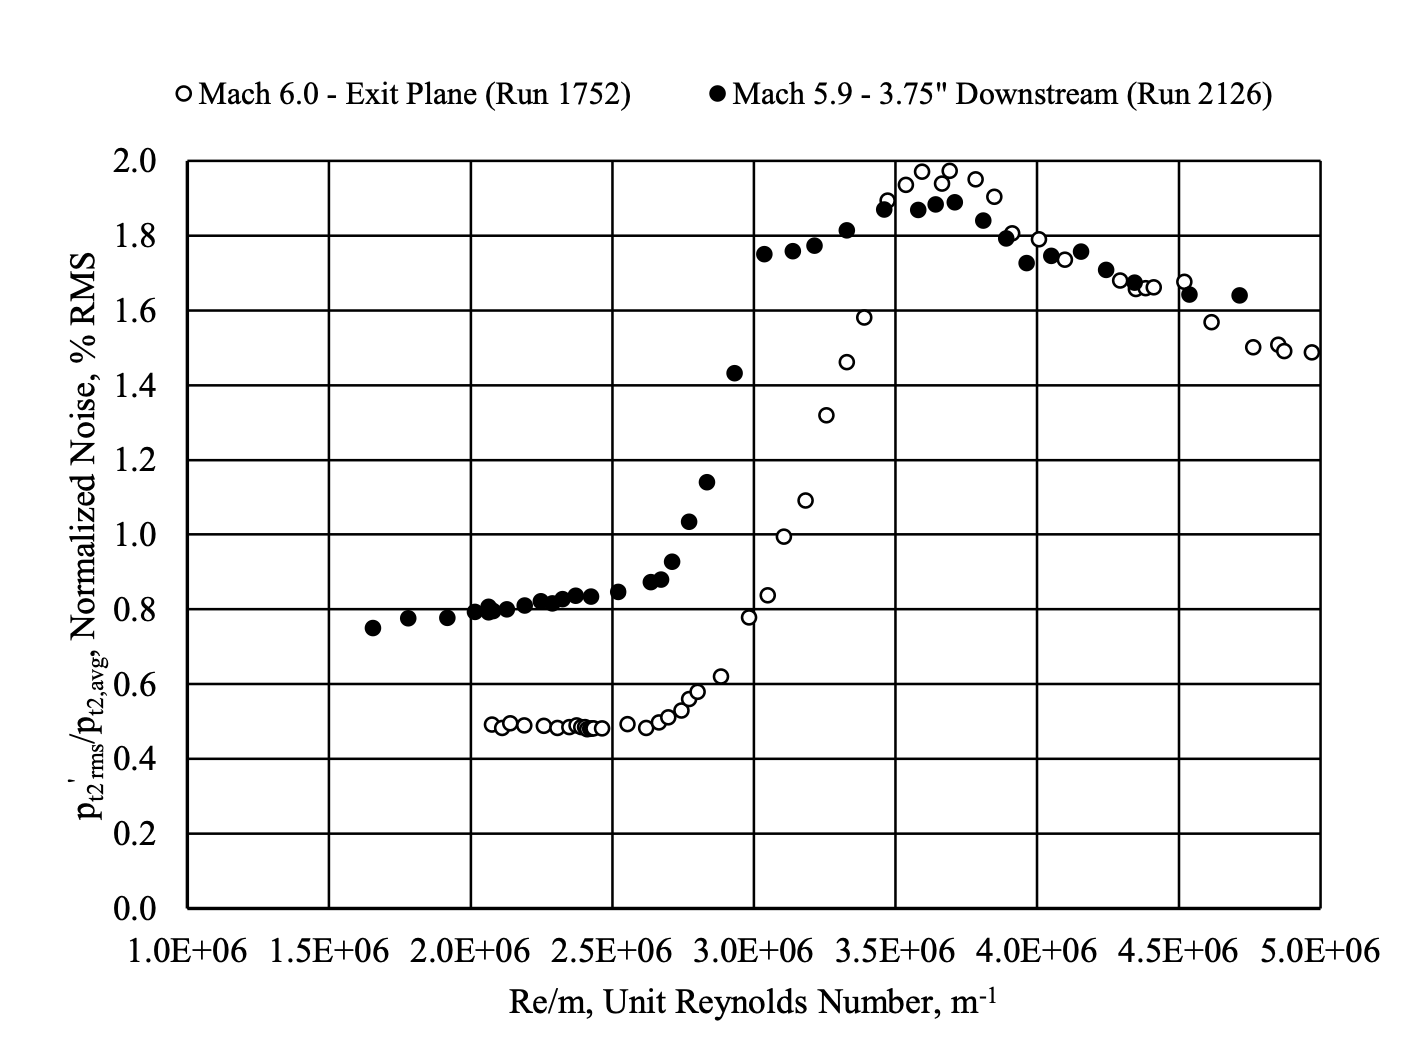
\includegraphics[width=5.5in]{mai-survey}
    \caption[ACE freestream pressure fluctuations in the nozzle exit plane as measured in 2014]{ACE freestream pressure fluctuations in the nozzle exit plane as measured in 2014 \cite{mai-dis}}
    \label{fig:mai-survey}
\end{figure}

\begin{figure}[ht!]
    \centering
    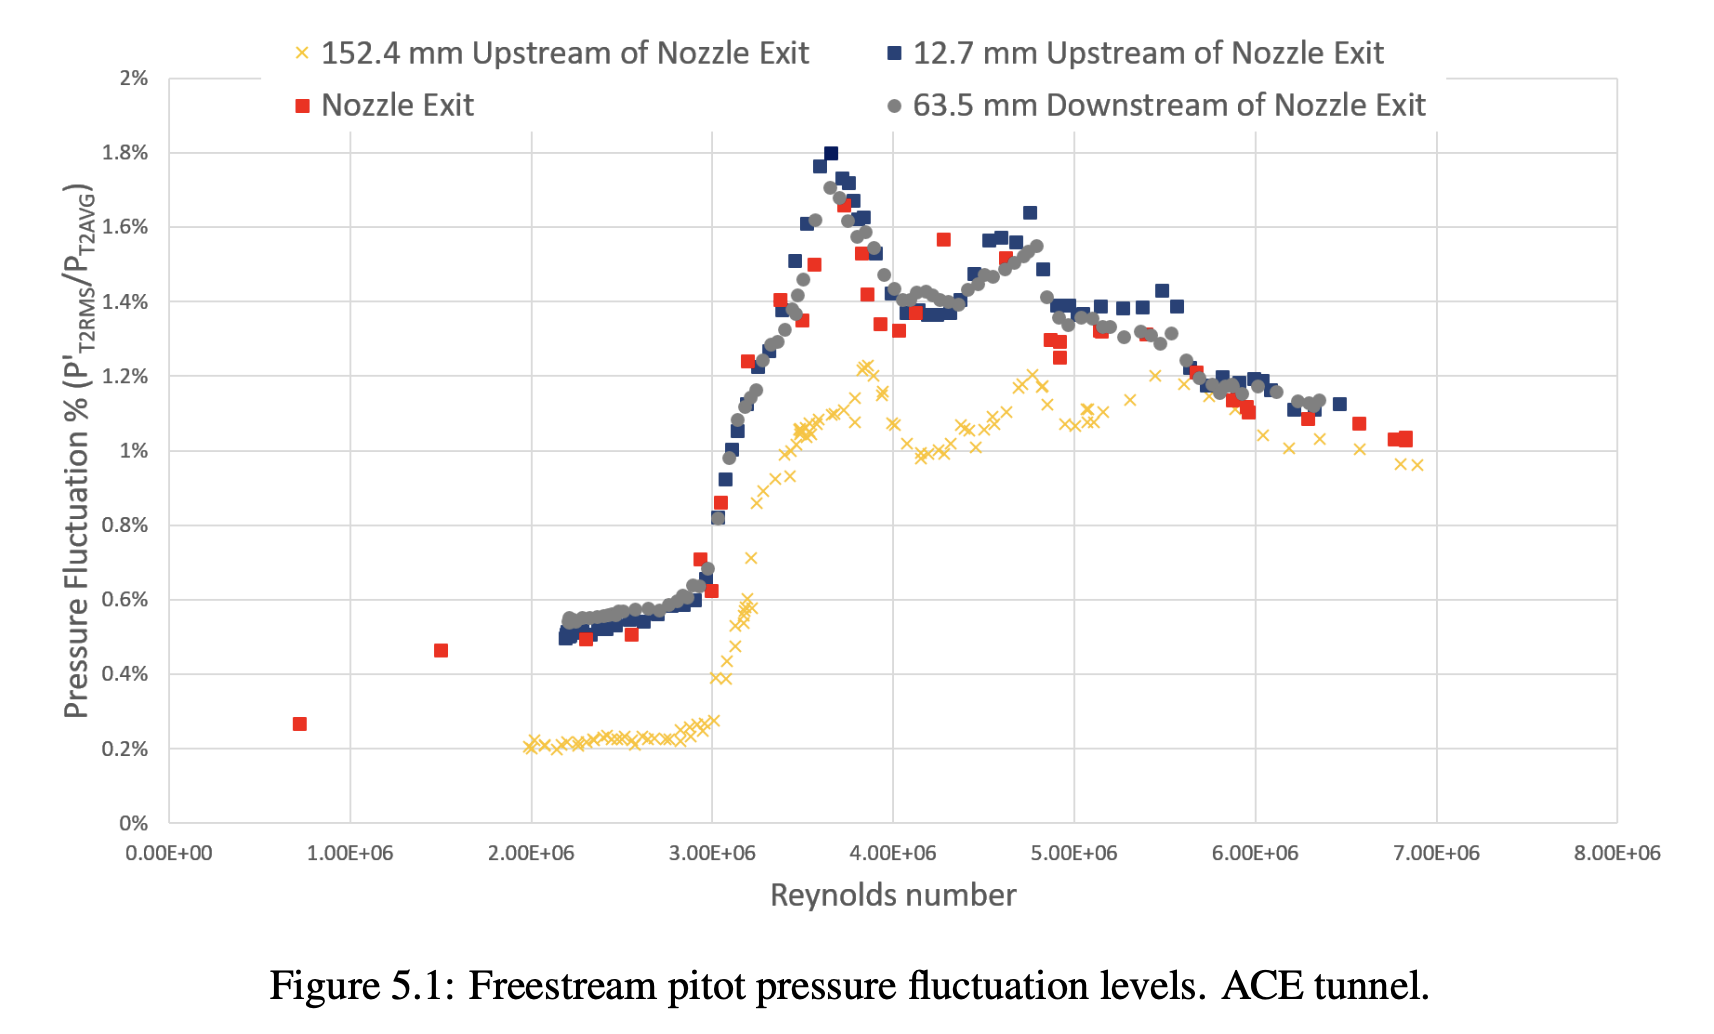
\includegraphics[width=6in]{neel-survey}
    \caption[ACE freestream pressure fluctuations at various locations as measured in 2019]{ACE freestream pressure fluctuations at various locations as measured in 2019 \cite{neel-dis}}
    \label{fig:neel-survey}
\end{figure}

\clearpage

\begin{figure}[ht!]
    \centering
    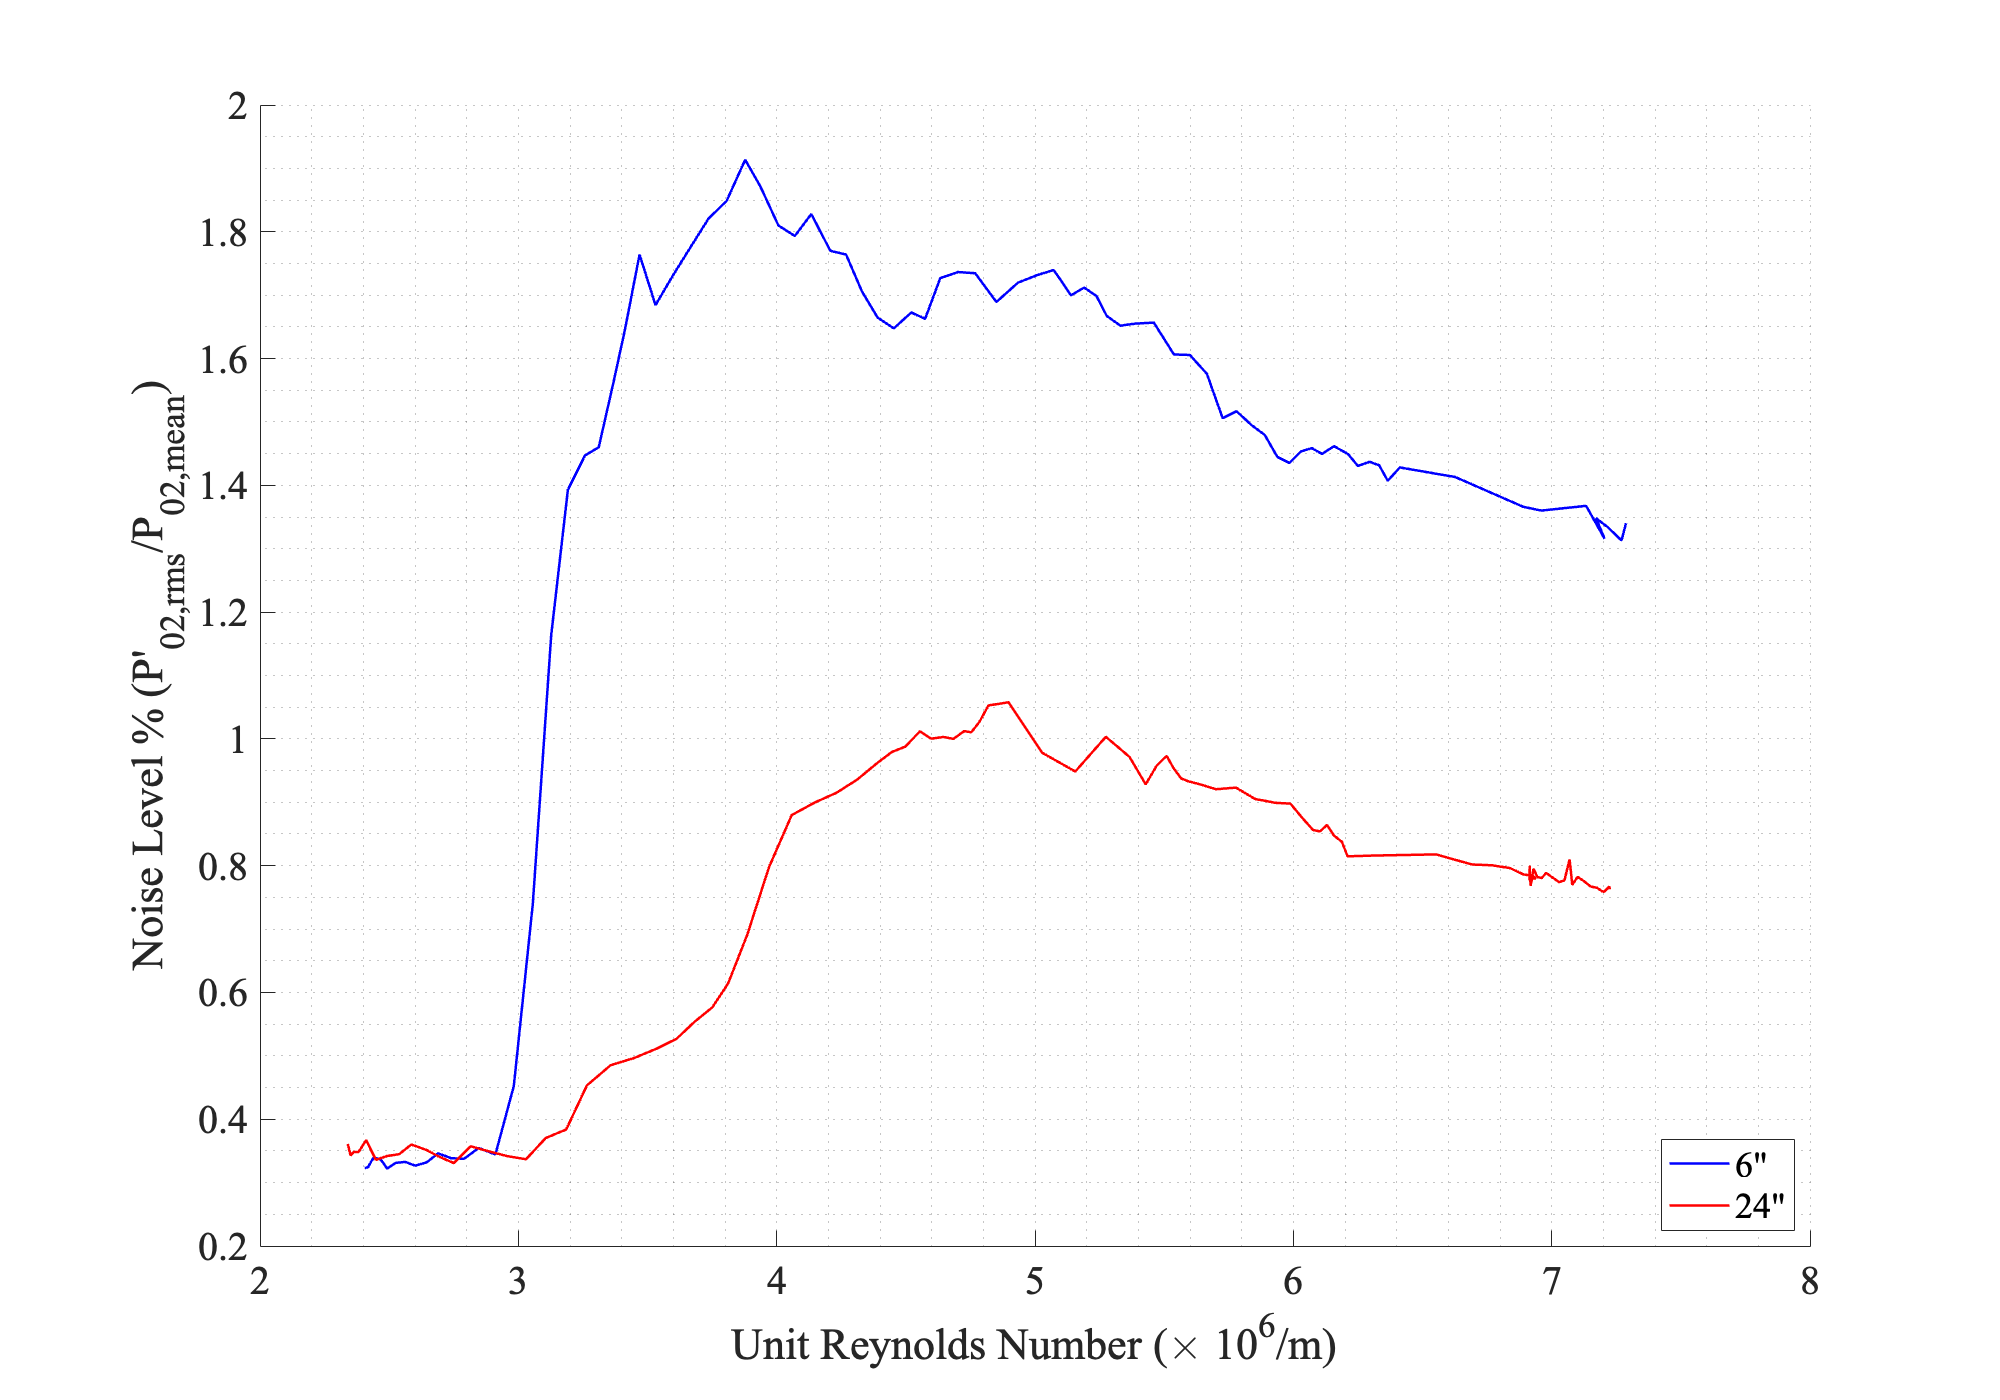
\includegraphics[width=5.5in]{ace-survey-2024}
    \caption{ACE freestream pressure fluctuations at 6 inches and 24 inches upstream of nozzle exit as measured in 2024}
    \label{fig:ace-survey-2024}
\end{figure}

\subsubsection*{Suspect Mechanism Conclusions}

The pressure fluctuation levels revealed the $Re'$ value at which transition occurs but not the transition mechanism. The two mechanisms that were extensively investigated at the start of this work were sidewall mushroom vortices and Görtler vortices. Sidewall mushroom vortices arise from the pressure distribution in the low momentum flow in the sidewall boundary layers. The flow at the centerline expands to the test section pressure ahead of the top and bottom curved walls. The flow at the top and bottom lags behind the centerline flow with a higher pressure to create a vertical pressure gradient that introduces a secondary vertical flow in the sidewall boundary layers that flows from the corners to the centerline \cite{sabnis}. CFD simulations by Kocian (unpublished) show the sidewall mushroom vortices beginning to form approximately 24 inches upstream of the nozzle exit shown in Figure \ref{fig:mushrooms}. 

\begin{figure}[ht!]
    \centering
    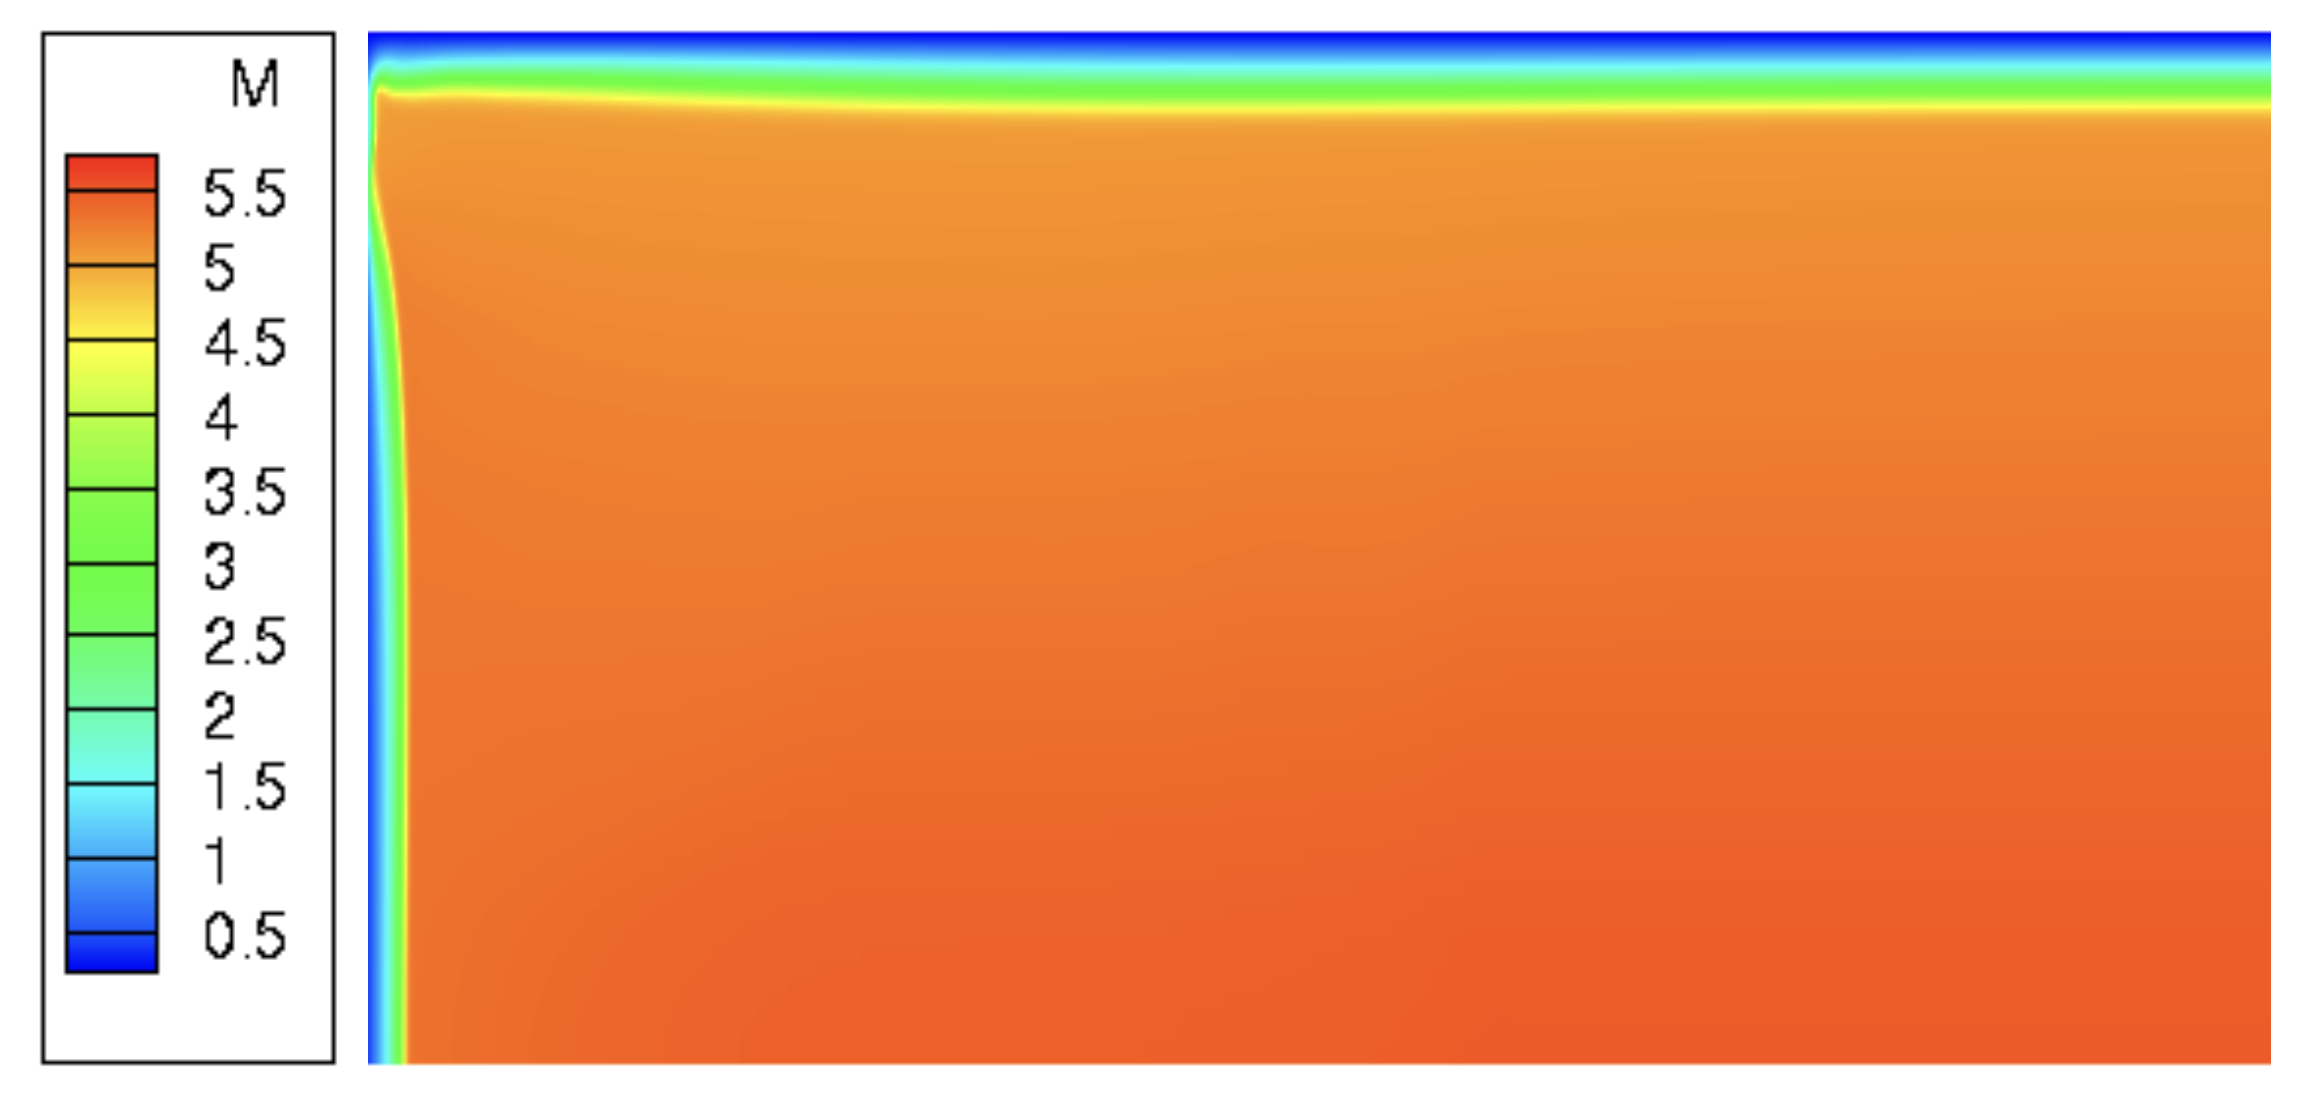
\includegraphics[width=4in]{mush24}
    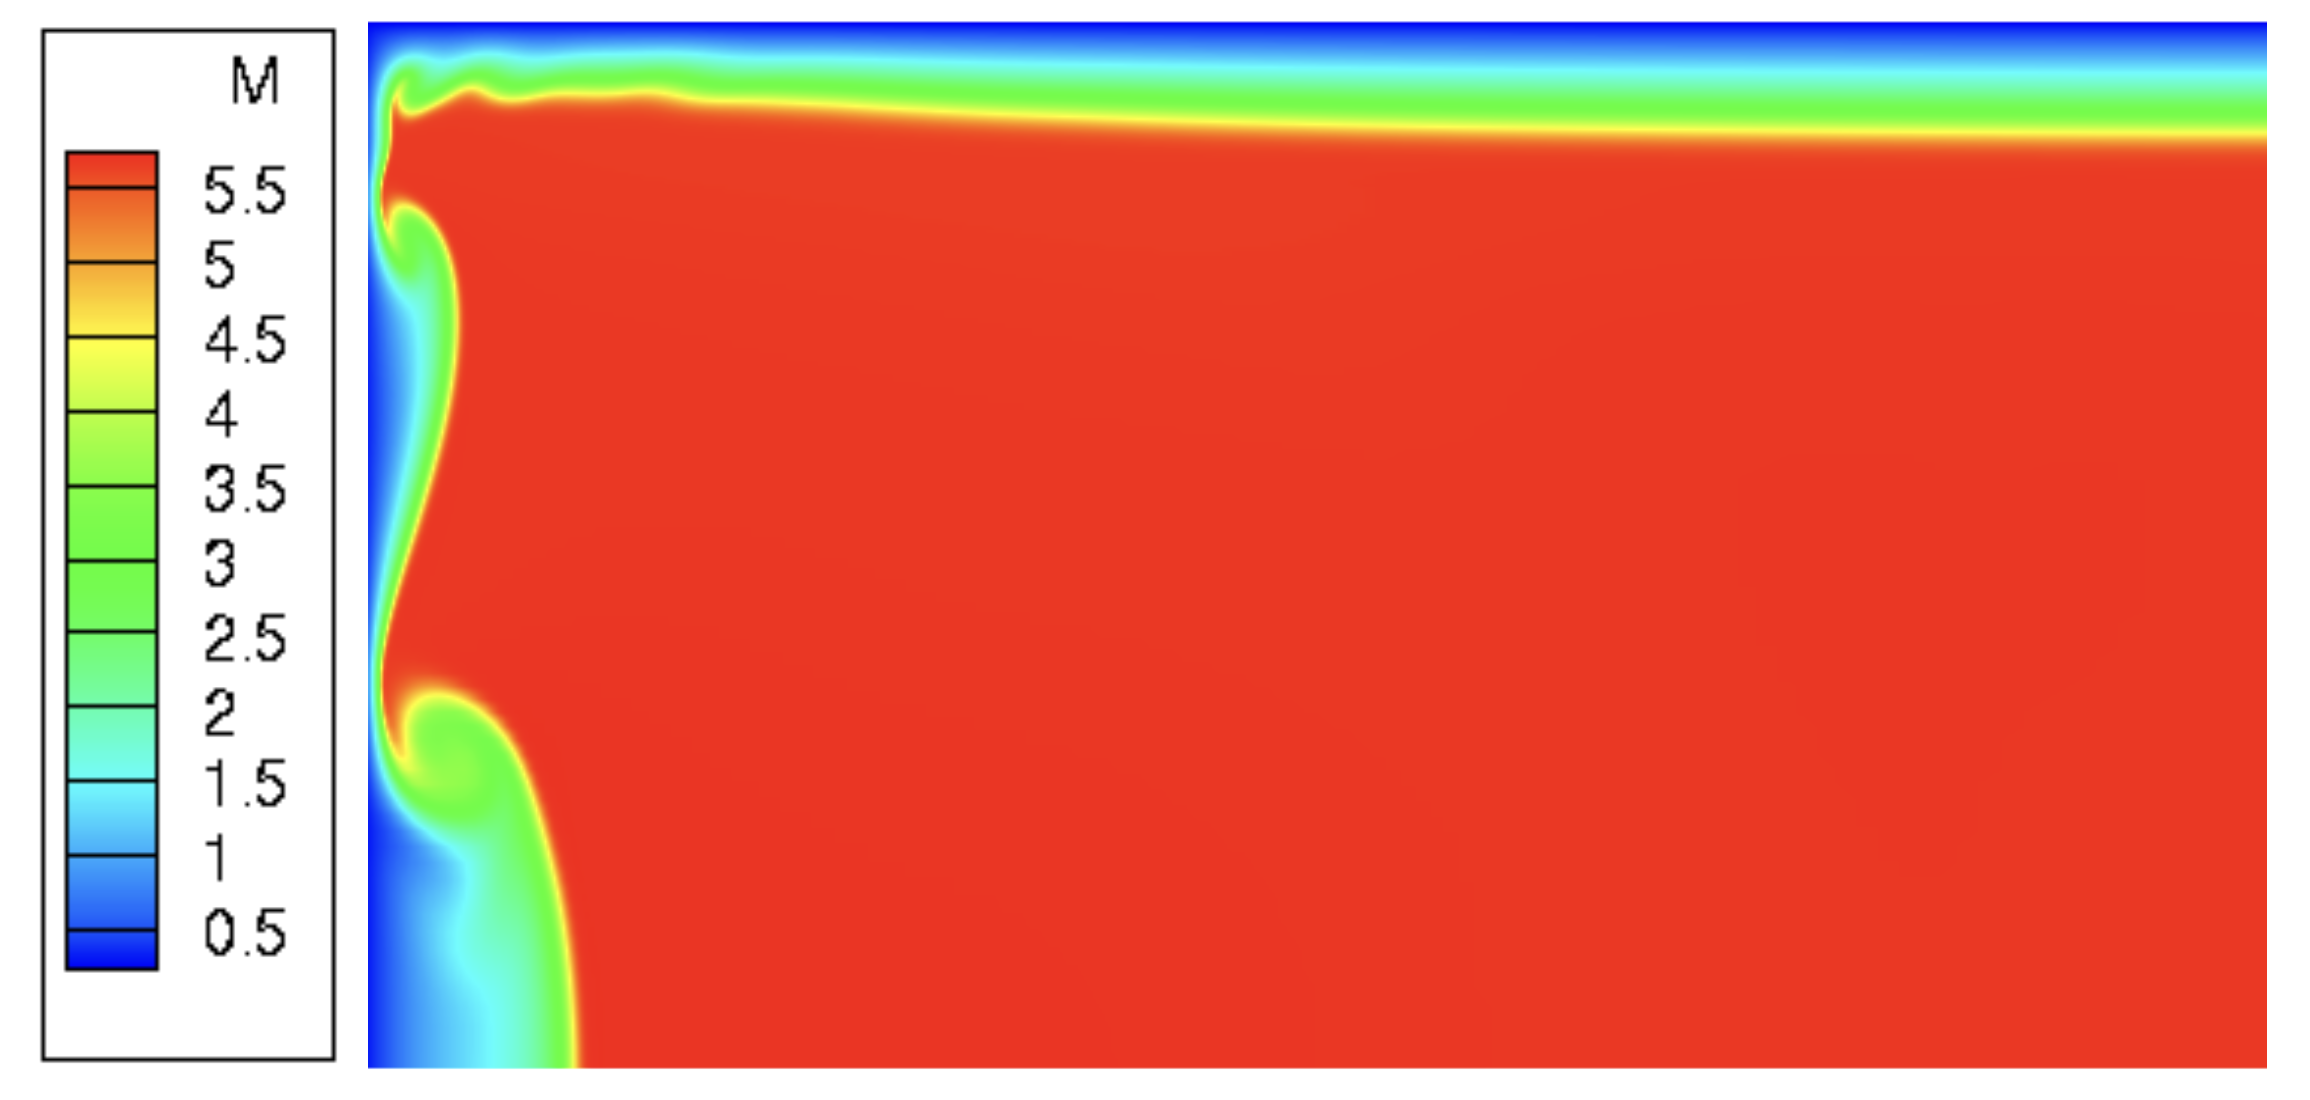
\includegraphics[width=4in]{mush0}
    \caption{Sidewall mushroom vortex formation (upper quarter) at 24 inches upstream of nozzle exit (top) and at nozzle exit (bottom) }
    \label{fig:mushrooms}
\end{figure}

Görtler vortices are counter-rotating streamwise vortices that occur in boundary layers on concave surfaces \cite{saric}. To estimate where these may lead to transition, a CFD basic state simulation and N-factor analysis was performed by Kocian in 2022 (unpublished). The results, shown in Figures \ref{fig:gortler} and \ref{fig:n-factor}, indicate that Görtler vortices could induce transition around 8 inches from the nozzle throat. 

\begin{figure}[ht!]
    \centering
    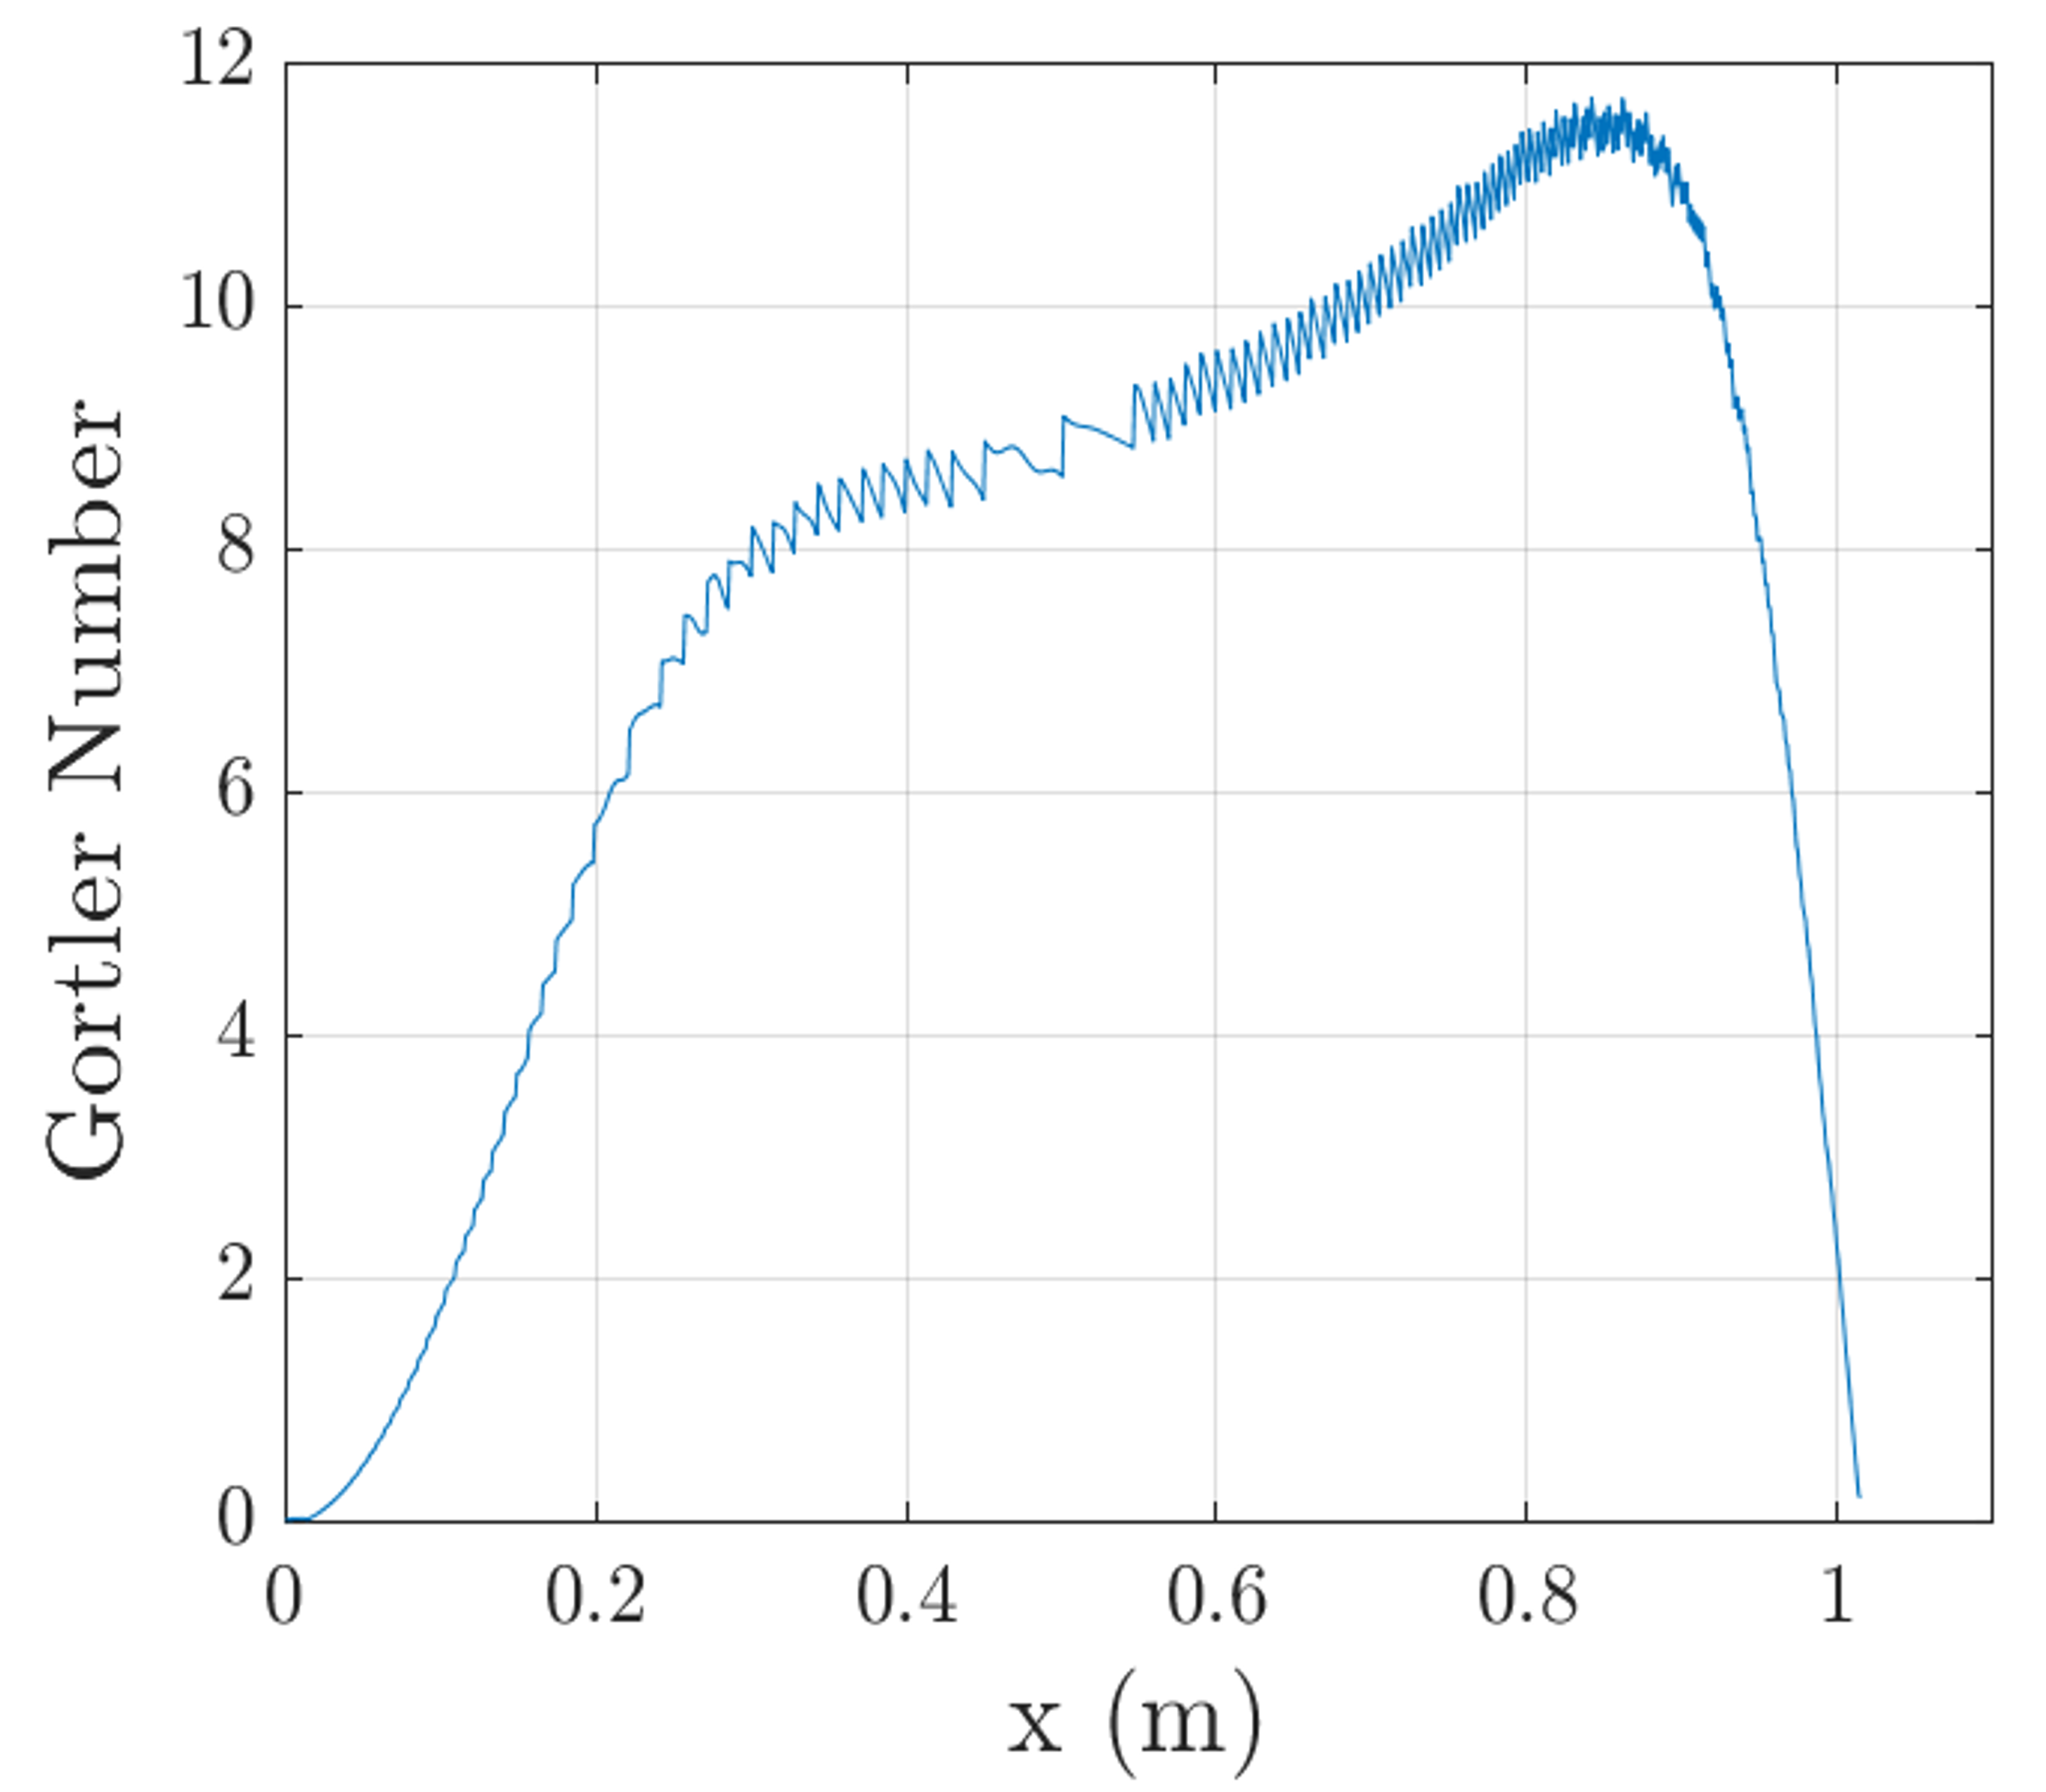
\includegraphics[width=4.2in]{gortler}
    \caption{Görtler number from ACE nozzle CFD}
    \label{fig:gortler}
\end{figure}

\begin{figure}[ht!]
    \centering
    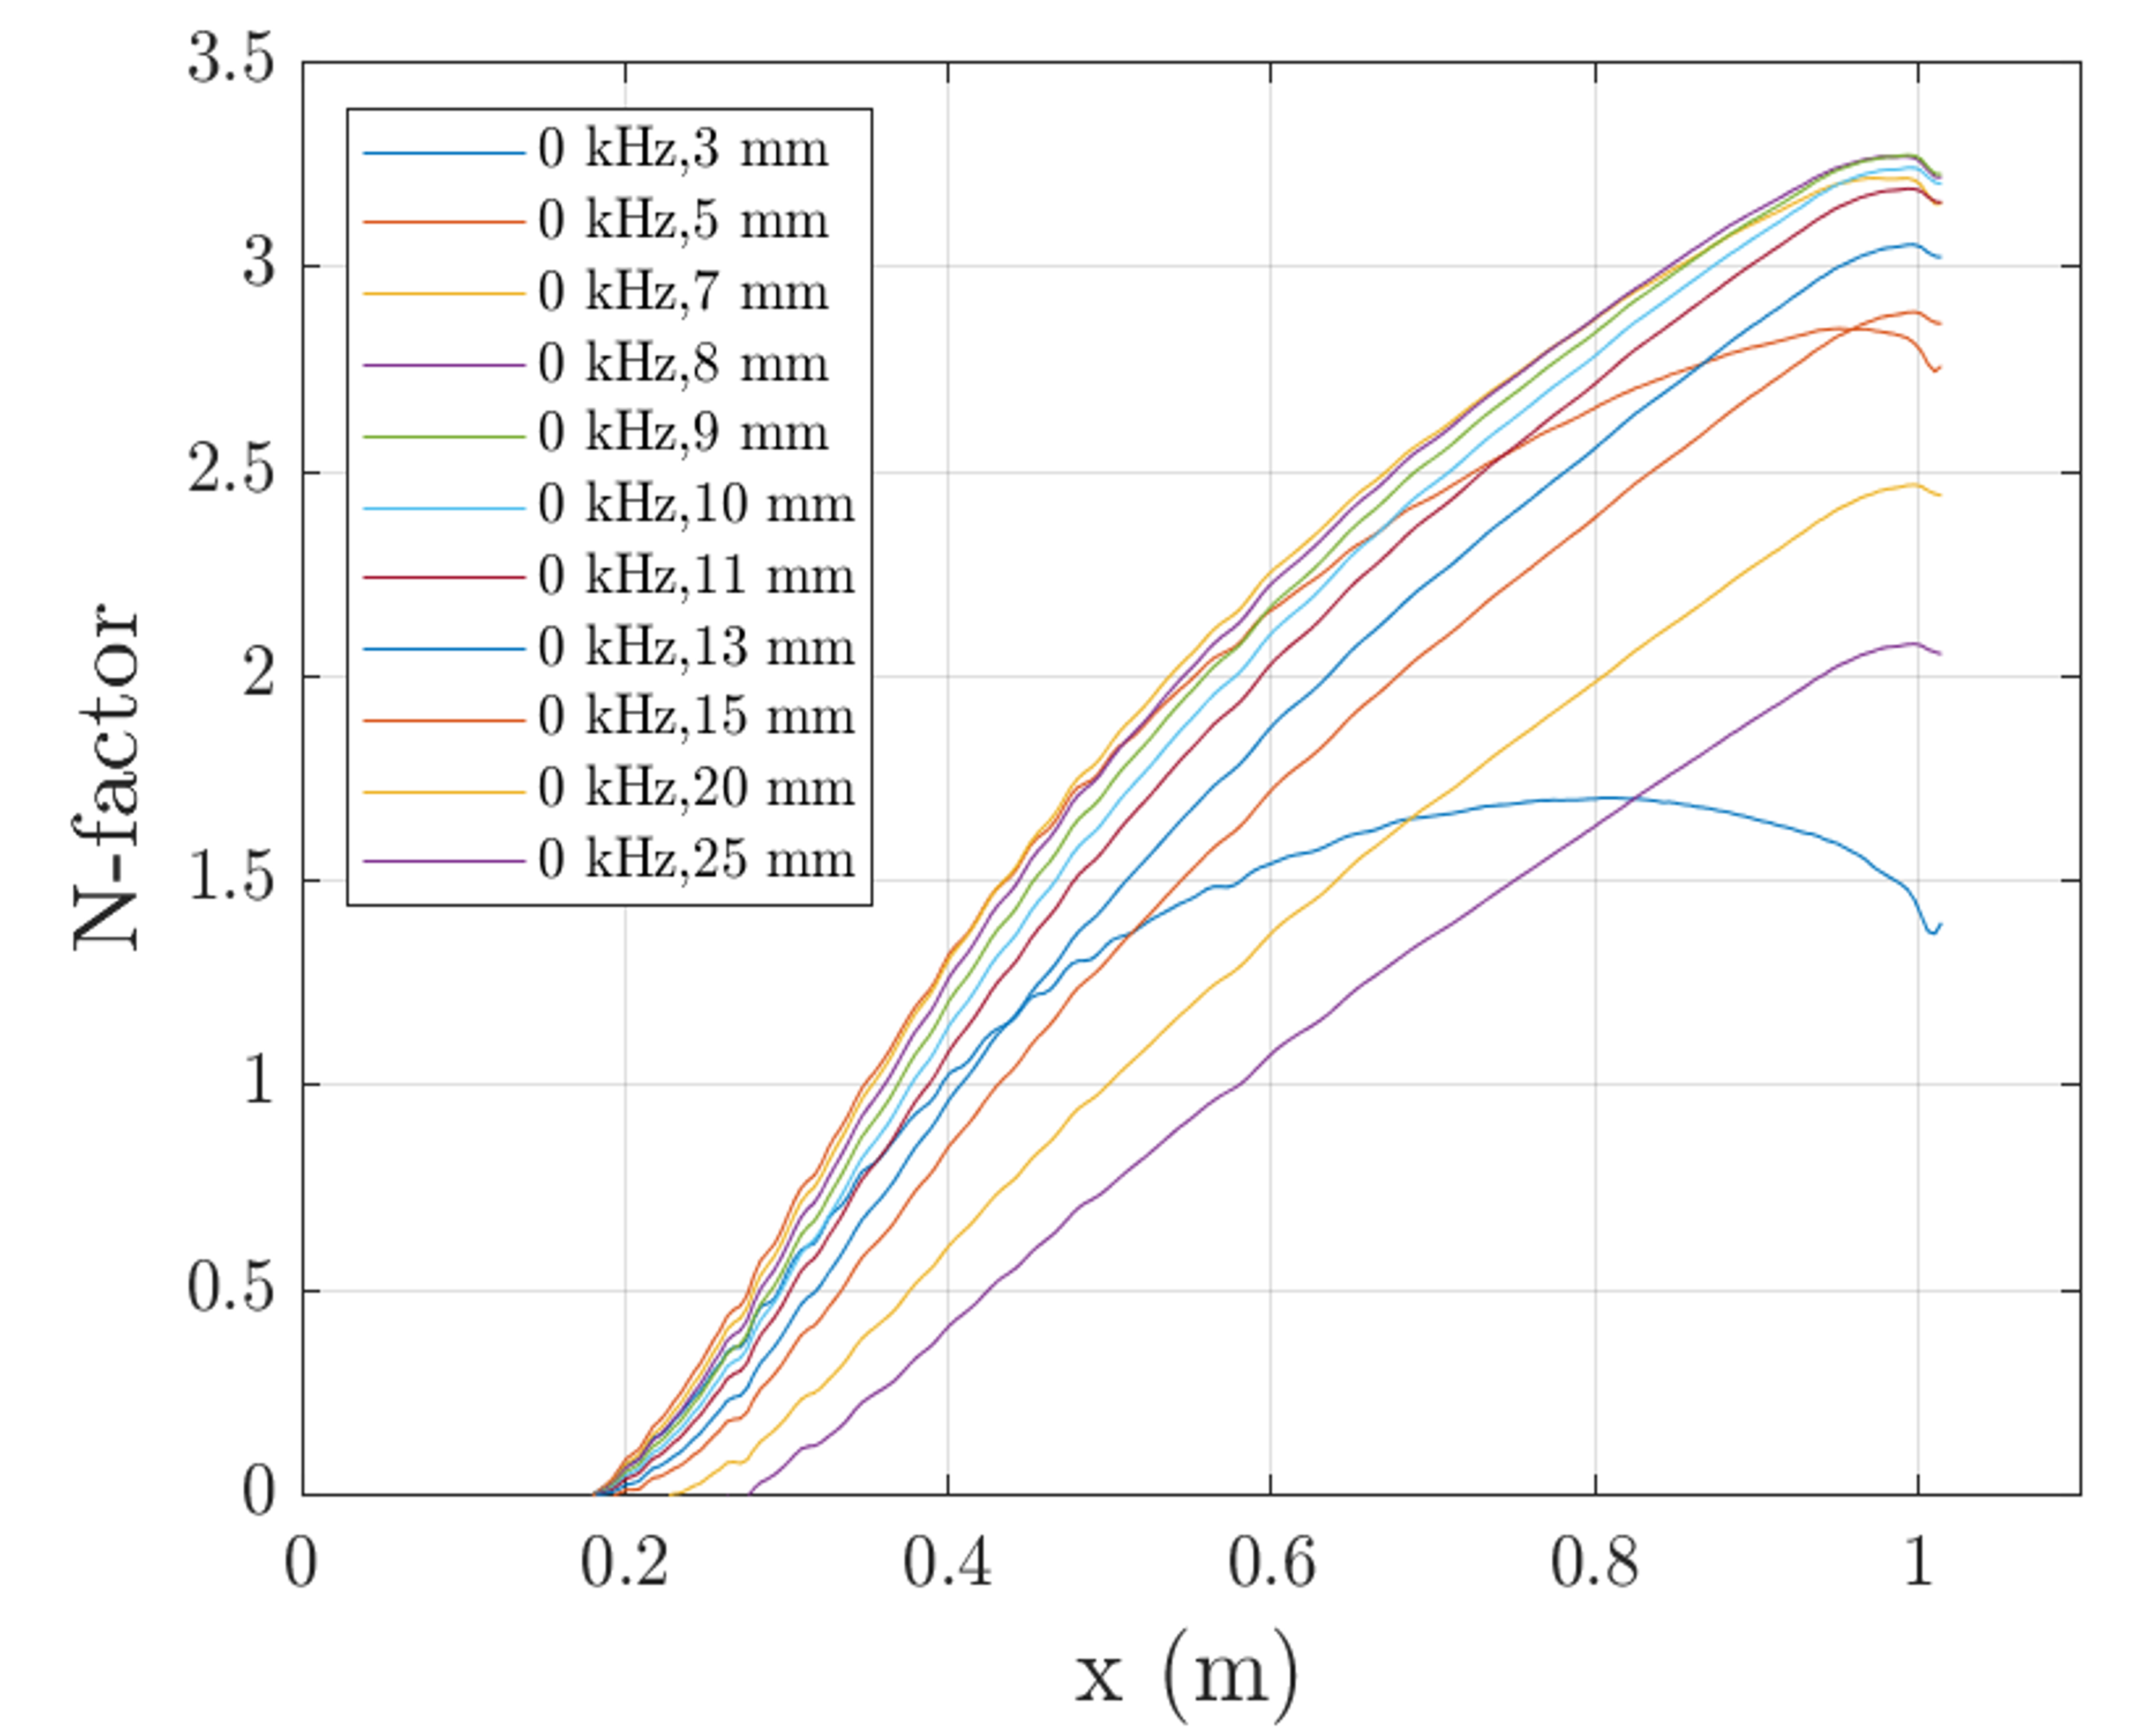
\includegraphics[width=4.2in]{n-factor}
    \caption{N-factors for Görtler in ACE nozzle}
    \label{fig:n-factor}
\end{figure}

The origin of the noise measured farthest upstream of the nozzle exit was determined by tracing characteristic lines from the measurement location at the centerline upstream to the wall. Both the side view and top view of this are shown in Figure \ref{fig:machlines}. This was accomplished by choosing the characteristic output by the MOC code that intersects the centerline closest to the measurement point of 24 inches and tracing it back to its origin at the wall. The origin of the measured noise from the top view is upstream of the throat where sidewall mushroom vortices are not relevant, and the origin of the noise from the side view is on the straight section of the nozzle where Görtler is not relevant. While both sidewall vortices and Görtler vortices can play some role in transition in planar nozzles, they are no longer considered suspects for the pressure fluctuation levels increase at unit Reynolds numbers above $3 \times 10^6/\mathrm{m}$.

\begin{figure}[ht!]
    \centering
    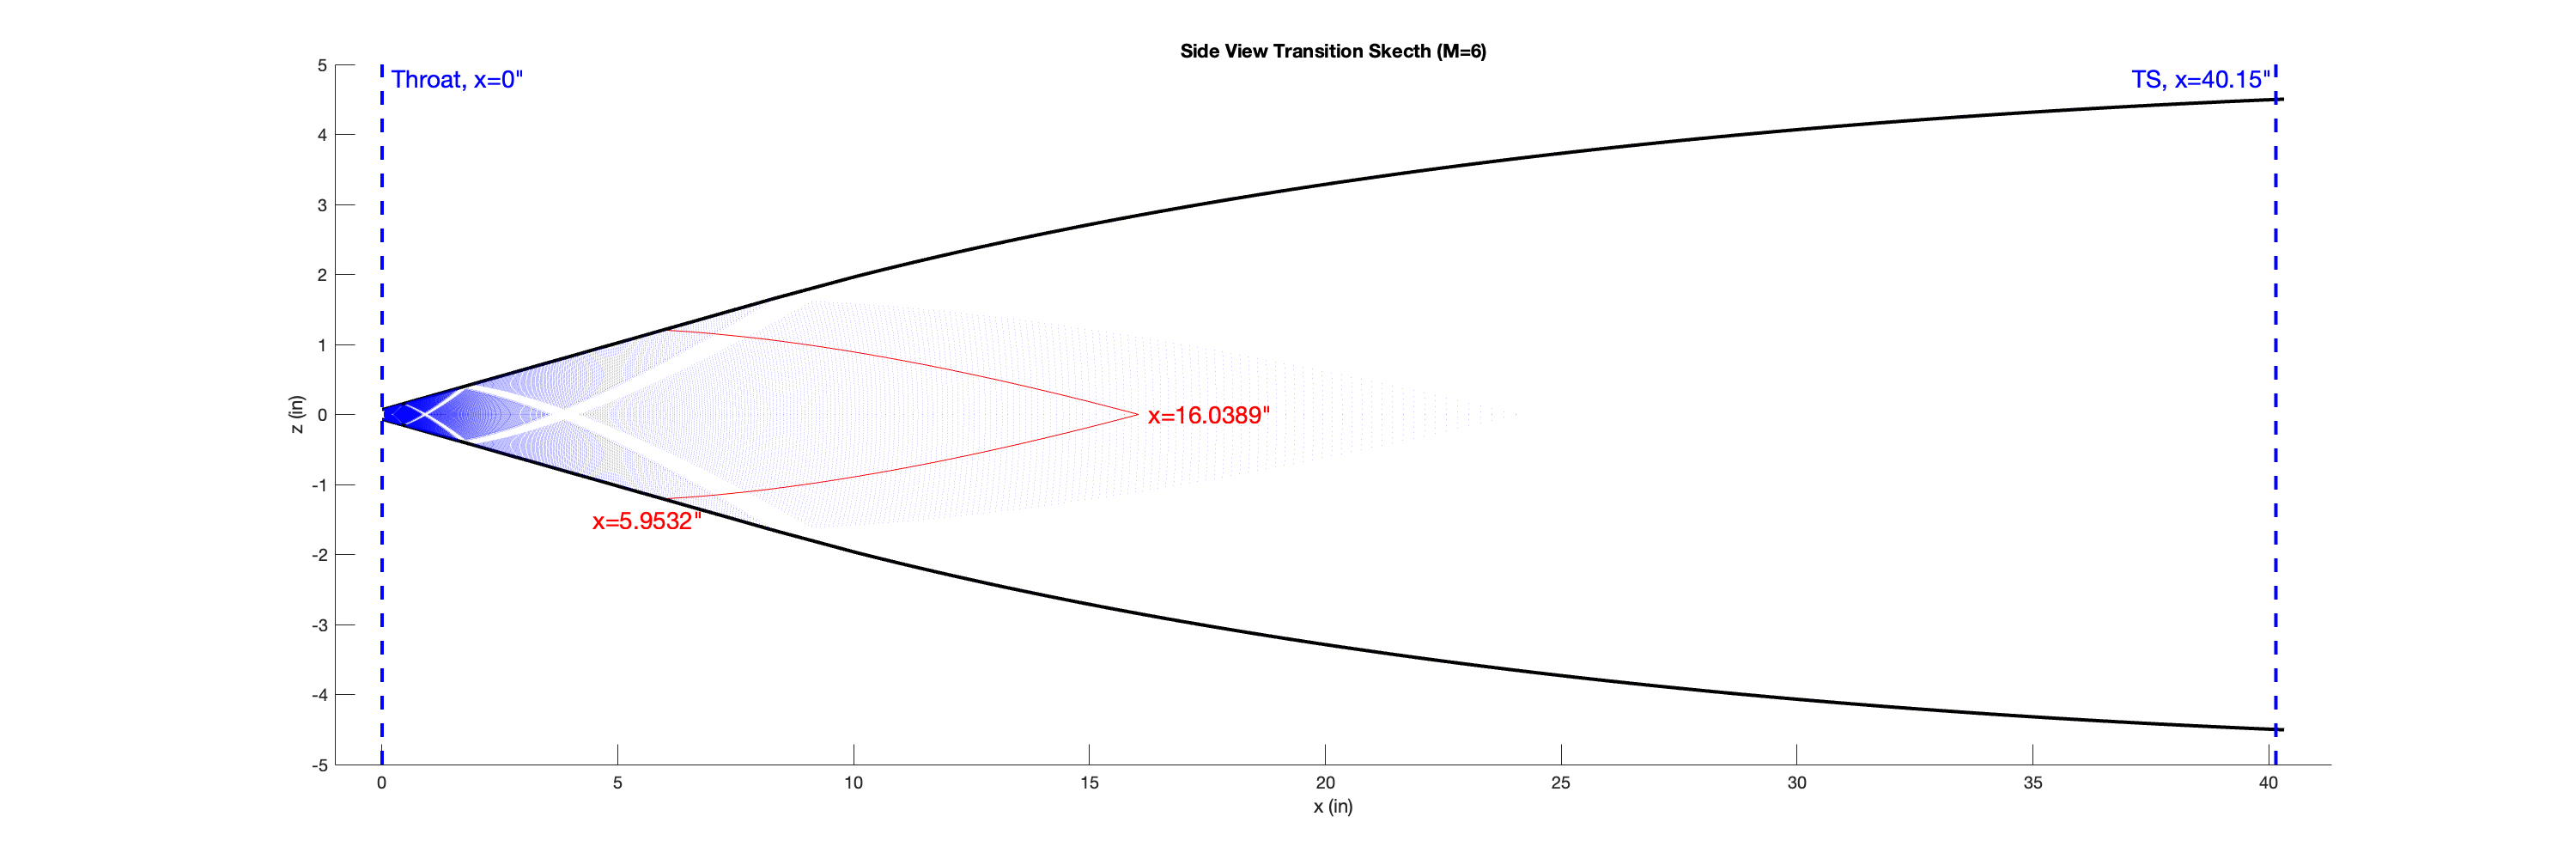
\includegraphics[width=6.5in]{side24}
    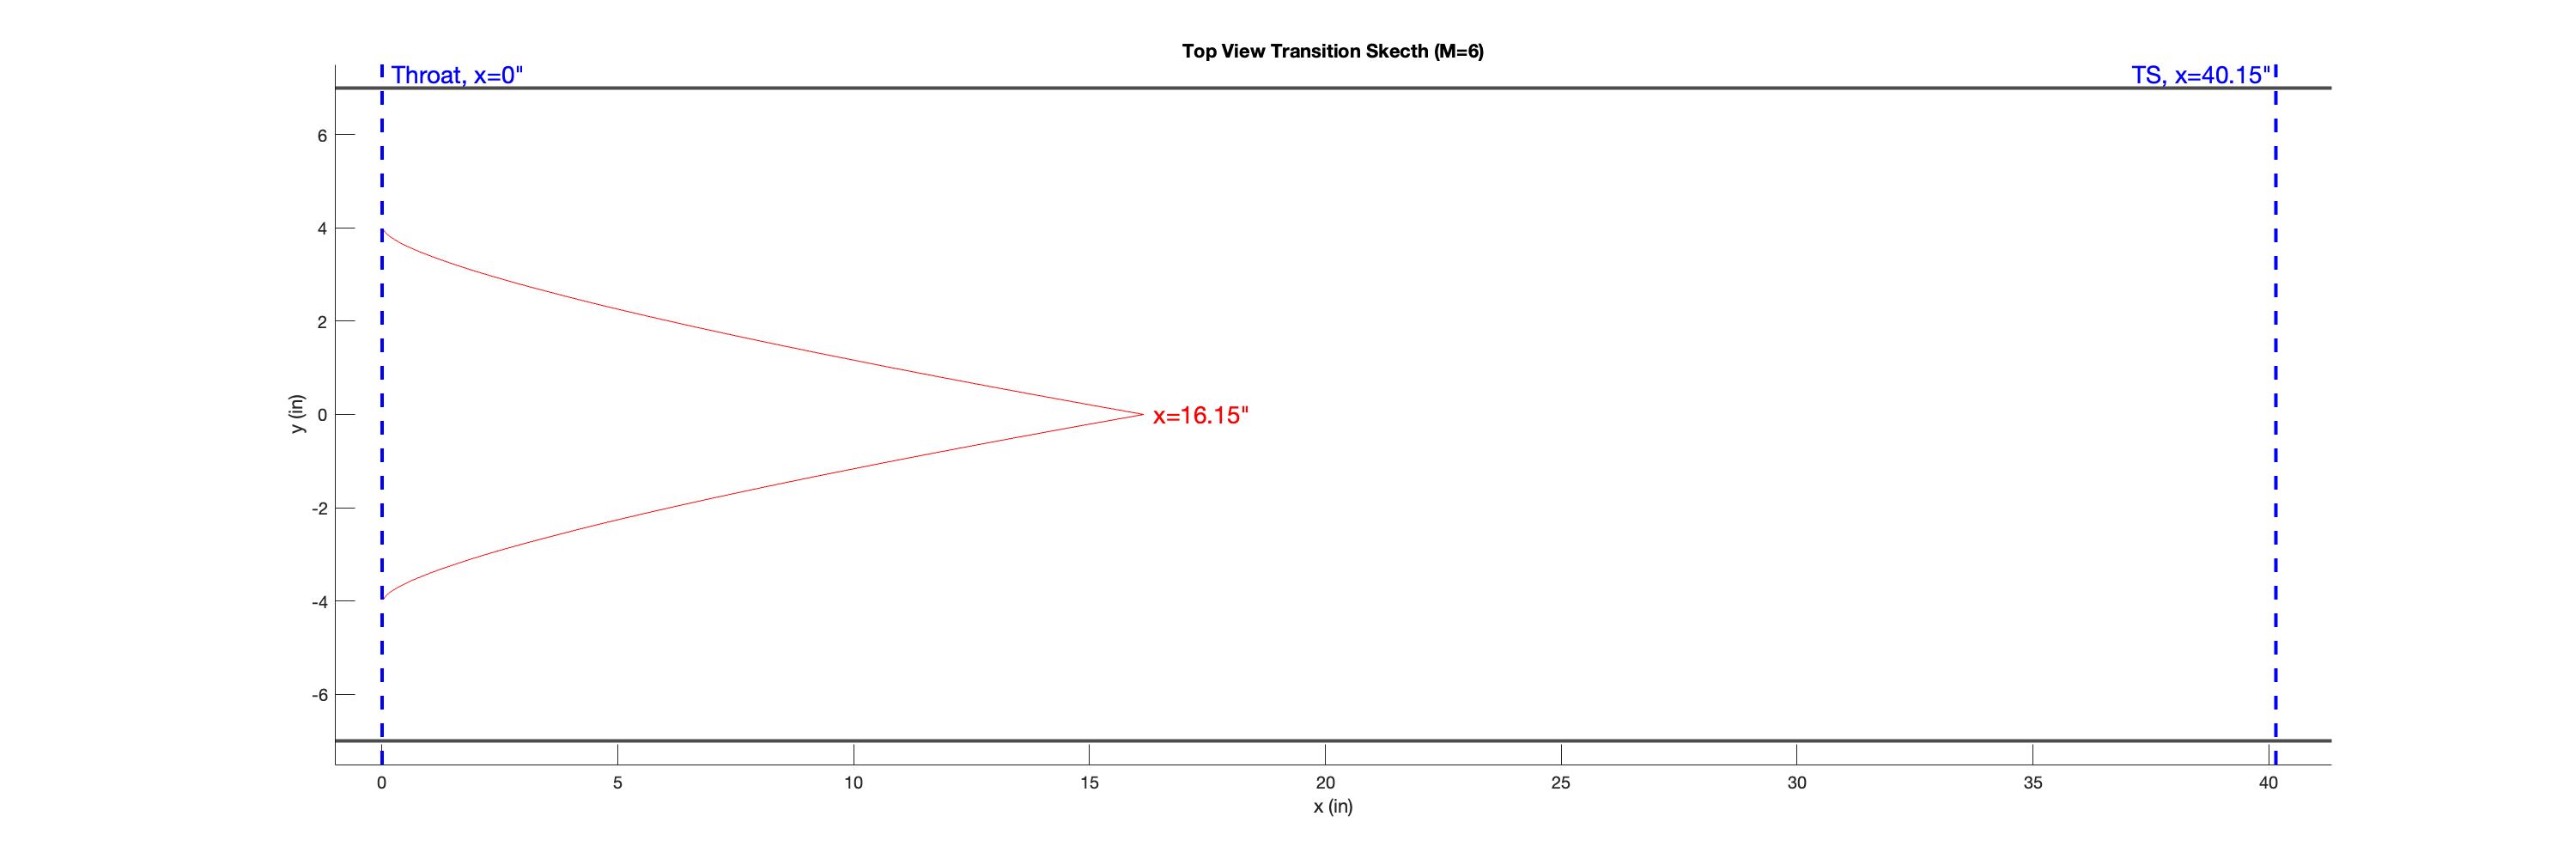
\includegraphics[width=6.5in]{top24}
    \caption{Mach lines for noise measured at 24 inches upstream on nozzle exit}
    \label{fig:machlines}
\end{figure}

Following the above conclusions and recommendations, the most likely reason the pressure fluctuations increase is laminar-to-turbulent transition due to a surface discontinuity at the throat. This conclusion is supported by pitot surveys, CFD, and method of characteristics line tracing described above. The remaining suspect mechanisms are still important to note and address in the redesign of the ACE tunnel. 

\subsubsection*{Design Recommendations}

The following improvements are recommended to maintain laminar flow above $Re'$ $\approx 3 \times 10^6/\mathrm{m}$:
\begin{enumerate}
    \item Second-derivative-smooth subsonic-to-supersonic throat transition to eliminate nozzle throat discontinuity
    \item Continuous curvature with analytical functions to eliminate waviness and surface discontinuities
    \item Enhanced surface polishing to minimize surface roughness
    \item Improved settling chamber design to maximize flow uniformity and minimize freestream turbulence upstream of the nozzle throat
\end{enumerate}

One recommendation that is outside the scope of this work is to incorporate subsonic boundary layer suction to greatly reduce the incoming noise and potentially make ACE2.0 a "quiet" facility. Boundary layer suction is quite complex to effectively implement, but it will be accommodated for in the design in case it is explored in the future. 

\section{ACE2.0 Design}

Following these recommendations, the nozzle will be redesigned and remanufactured to meet specific requirements that will ensure the best performance and potentially expand the laminar Reynolds number range. The decision to remanufacture the nozzle presents an opportunity to revise the nozzle and settling chamber design to achieve true active controllability, properly embodying the "ACE" name.

The rest of the chapter details the planned improvements to the ACE tunnel and specific design requirements that will achieve those improvements. In addition to a new nozzle, the settling chamber will also be redesigned to ensure the uniformity and reduce the turbulence of the flow into the nozzle. These improvements are to achieve the goal of increasing the unit Reynolds number at which laminar nozzle flow is maintained.

\subsection{Design Requirements}

ACE2.0 will maintain many characteristics while improving some, so many requirements are the same as the original ACE design. The new tunnel will still produce uniform Mach 5 to 8 flow in the 9 inches by 14 inches test section, withstand a total temperature of 530 K, and maintain a minimum engineering factor of safety (FOS) of 1.5 when operating at a total pressure of 200 psia.

\subsubsection*{Nozzle Requirements}

The current ACE nozzle successfully produces uniform Mach 5 to 8 flow in its core. In order to maintain this good performance and not introduce unknown parameters, the new nozzle will retain a very similar contour with slight improvements. The requirements that remain the same are that the nozzle must produce uniform flow for the entire Mach range, achieve maximum height deflection with a minimum FOS of 1.5, and prevent leaks up to 200 psia.

The improvements to the nozzle and associated requirements will be a contour with continuous 1st and 2nd derivatives that is specified by analytical functions that will eliminate discontinuities and truncation error and a maximum allowable stress less than or equal to that found in the current ACE flexure at maximum deflection.

\subsubsection*{Settling Chamber Requirements}

The current ACE settling chamber design provides multiple opportunities to improve flow conditioning and ease of maintenance. The new settling chamber design will increase the length and height and allow for variable aerogrid/screen configurations. The requirements that remain the same are low freestream turbulence, thin stable wall boundary layers, maximum uniformity, and preventing leaks at a pressure of 200 psia. The implementation of these requirements will be improved in the new design to achieve improved incoming flow into the nozzle.

Following Reshotko et al. \cite{reshotko}, the length of the settling chamber shall accommodate a separation of 250 characteristic mesh sizes between screens allowing for adequate turbulence decay. The aerogrids will have a hexagonal perforation pattern to increase porosity and decrease pressure loss. The number of aerogrids and screens shall be variable to allow for future flow conditioning experiments. The inlet shall include a baffle system that will provide an acceptable initial distribution and mixing of the air received from the high-pressure inlet piping. The overall design will accommodate the option for future boundary layer suction slots.

A settling chamber height of 6 inches was chosen to keep the velocity as slow as possible without going below 10 ft/s for the majority of the Mach number range. Pope and Goin \cite{pope} describe that this minimum prevents thermal convection vortices from dominating the flow at the walls. The interior of ACE2.0 will also be heated prior to the start of the run to help avoid thermal gradients. 

\subsection{Nozzle Contour Codes}

The multiple reflections method-of-characteristics (MOC) Fortran script by Bowersox that produced the ACE nozzle contour was used for the new nozzle contour. In order to achieve continuous first and second derivative continuity, a section of the code was modified to produce a fourth-order expansion section instead of the original second-order curve. This allowed the expansion section to match the curvature of both the subsonic section and the straight section. The code modification is included in Appendix \ref{appendix:contour}, and a comparison of the original quadratic and the new quartic expansion sections is shown in Figure \ref{fig:throats}. In this figure, the ACE contour is directly from the MOC points and the ACE2.0 contour is specified by an analytic fourth-order polynomial. The waviness of the MOC points can be seen here, emphasizing the need to define the entire nozzle with analytic functions.

\begin{figure}[ht!]
    \centering
    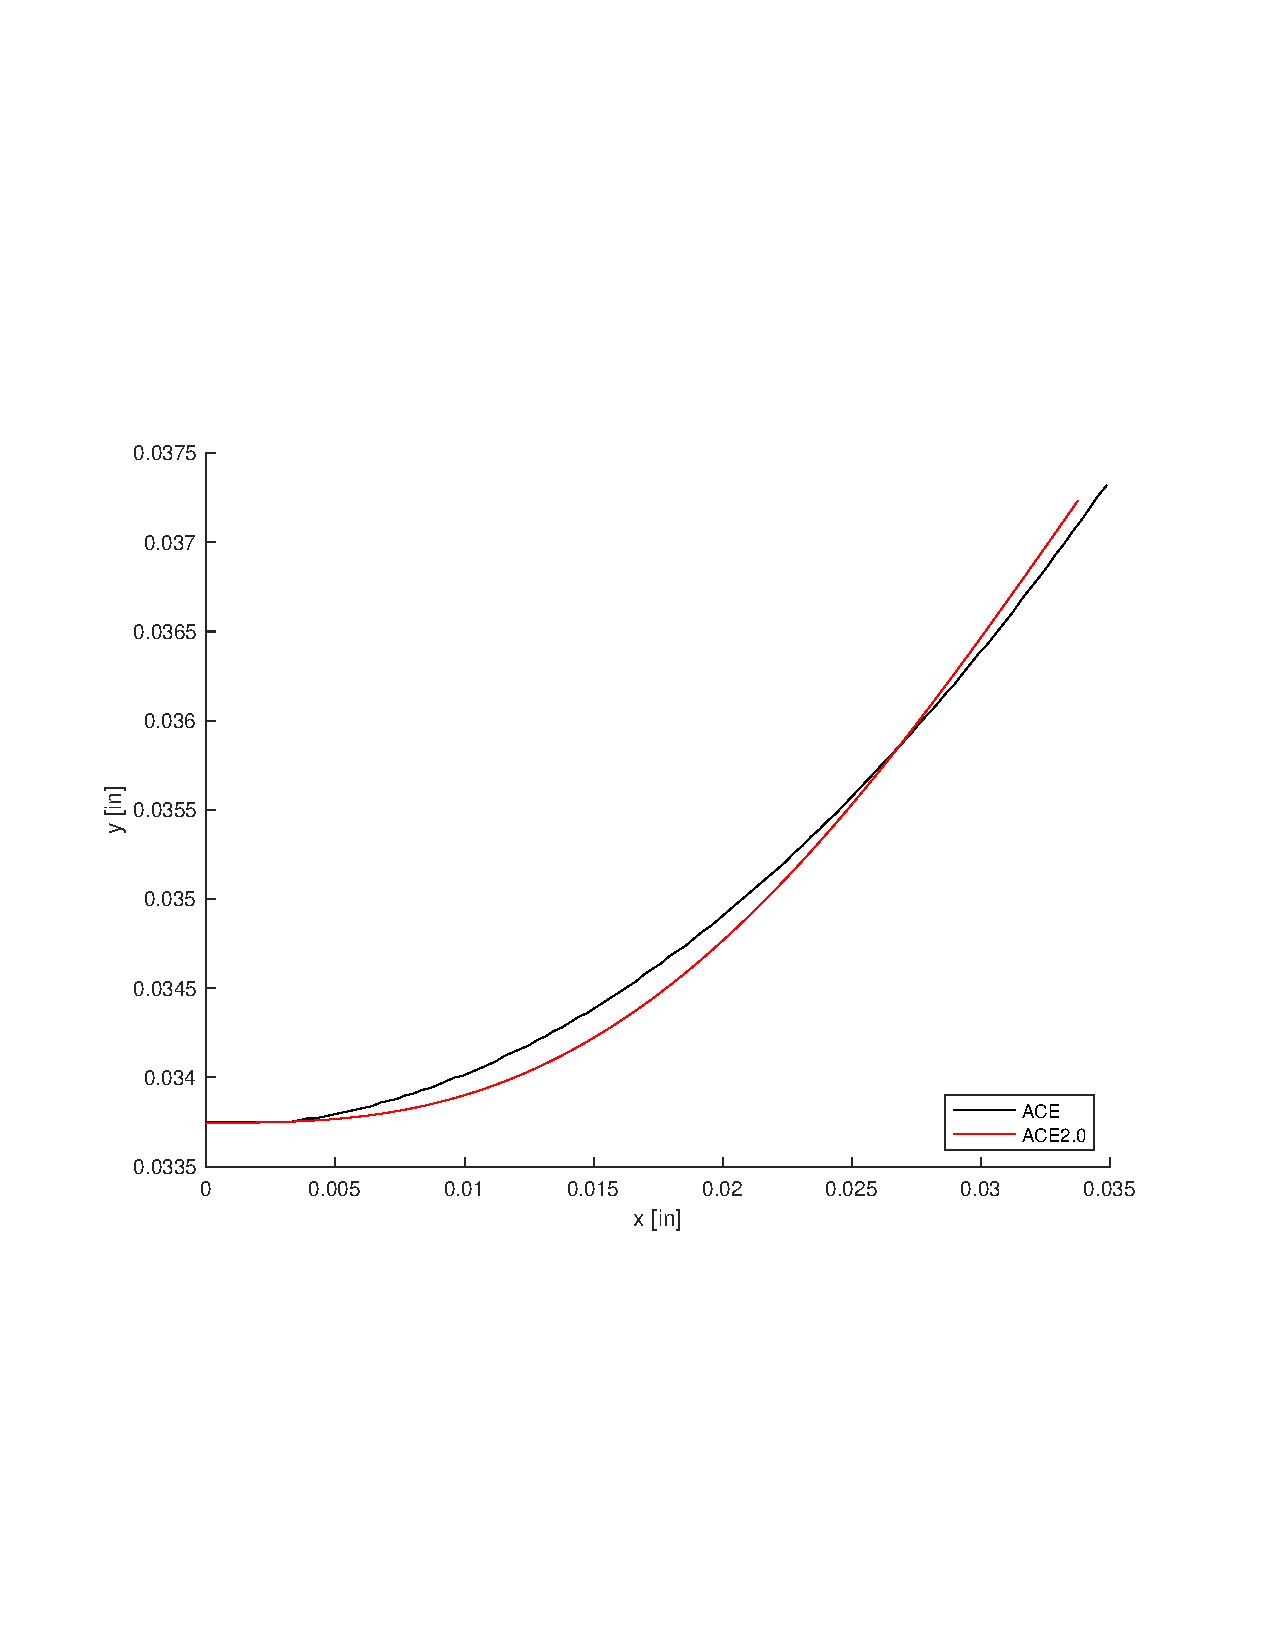
\includegraphics[trim={50 200 50 200},clip,width=6in]{throats.pdf}
    \caption{Comparison of ACE (quadratic) and ACE2.0 (quartic) expansion at throat}
    \label{fig:throats}
\end{figure}

After the MOC points were produced by the Fortran script, they were imported into a MATLAB script to fit with analytic functions. The subsonic curve is given by a fifth-order polynomial with six boundary conditions of the settling chamber and throat heights and zero slope and curvature at both the start and throat. The straightening section is given by a function found using the \texttt{lsqcurvefit} function with a combination of power and logarithmic functions in MATLAB. The equations for each section are given in Appendix \ref{appendix:contour}.

\subsection{CFD}

In order to verify the above nozzle contour performance compared to the original ACE contour, both contours were simulated in 2D CFD. First, a mesh was created in Pointwise for each contour with 400 equally spaced columns of cells in the x-direction. Each column had the spacing scaled to accurately capture the boundary layer with the smallest cell height around $4 \times 10^{-6}$ inches at the curved wall and the largest around 0.2 inches at the centerline as seen in Figure \ref{fig:mesh}. The CFD analysis was performed at a time when the settling chamber design was still at a height of 9 inches, so the analysis will be performed again to validate the 6 inch.

\begin{figure}[ht!]
    \centering
    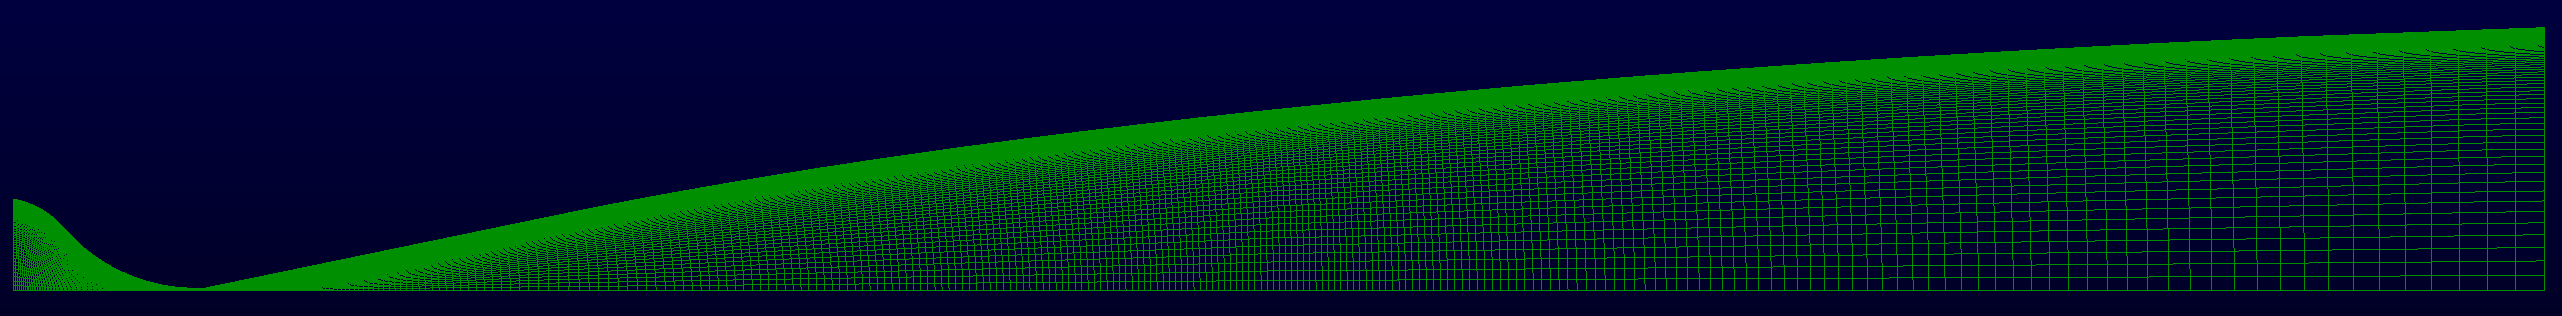
\includegraphics[width=6in]{ace-mesh}
    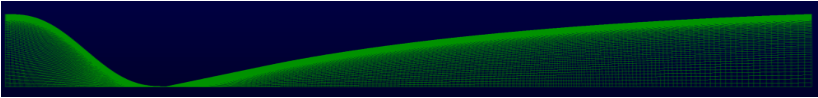
\includegraphics[width=6in]{qace-mesh}
    \caption{Mesh in Pointwise for ACE (top) and ACE2.0 (bottom) nozzle contours}
    \label{fig:mesh}
\end{figure}

After creating a mesh for each, they were simulated using US3D on the Texas A\&M supercomputer, Grace. A sample of the results is shown in Figure \ref{fig:ace2-cfd}. The full ACE2.0 CFD input conditions and results compared to ACE will be provided in a future appendix after performing the revised simulations in future work.
%is given in Appendix \ref{appendix:cfd}.

% \textcolor{red}{Stuff about inputs and convergence conditions...} 

\begin{figure}[ht!]
    \centering
    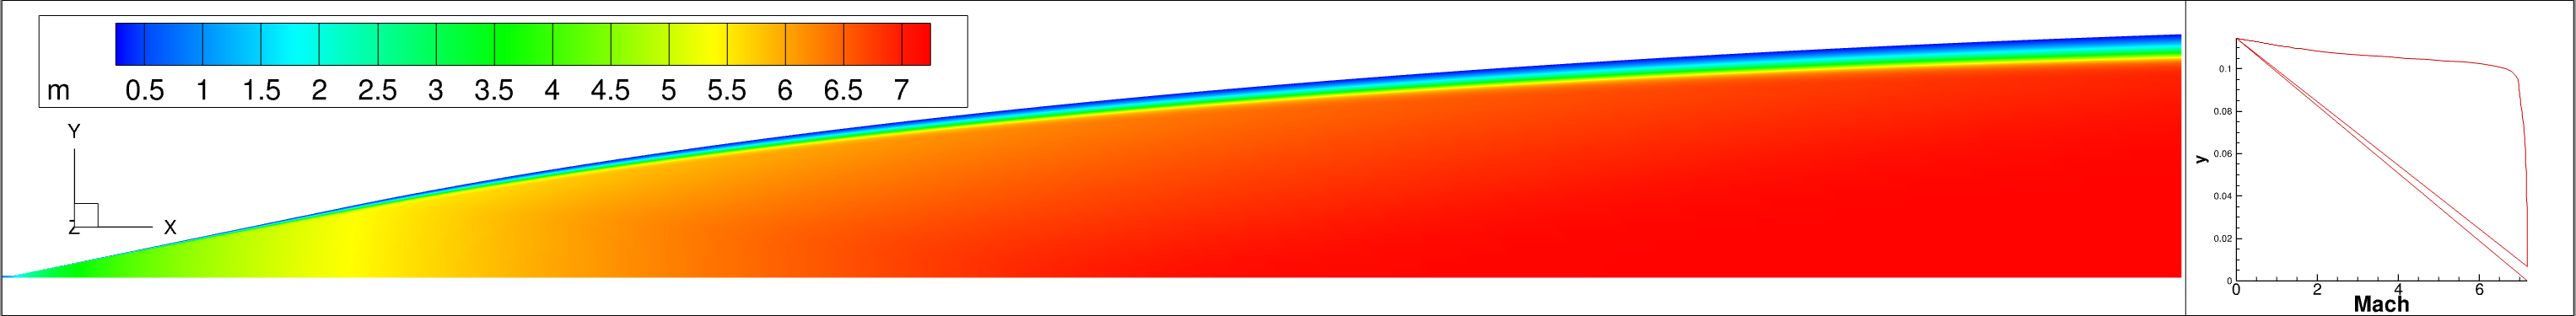
\includegraphics[width=5.5in]{ace2-cfd}
    \caption{ACE2.0 CFD Mach number distribution at exit plane}
    \label{fig:ace2-cfd}
\end{figure}

\subsection{General Nozzle and Settling Chamber Design}

The resulting contour from above was imported into Solidworks using the analytic equations given in Appendix \ref{appendix:contour}, and the new ACE2.0 nozzle and settling chamber were designed following the above requirements. In order to accommodate the active control, the nozzle and settling chamber were combined into single rigid upper and lower pieces. Similar to ACE, the last 4 inches of the nozzle is a separate flexure piece to enable the variable Mach number capability. The overall length of the nozzle and settling chamber was increased by 19 inches with most of the added length contributed to the settling chamber. The settling chamber is 1.7 inches taller and has a few considerable improvements described in a later section. 

The ACE design had the relative motion interface between nozzle and settling chamber with a large rubber seal that struggled to properly seal at higher Mach numbers. For ACE2.0, the end of the settling chamber is split into two pieces to allow the rotation of the nozzle blocks. This moves the potential sealing issue upstream of the flow conditioners where minor leaks are much less of a concern. The final ACE2.0 nozzle and settling chamber design compared to ACE is shown in Figure \ref{fig:nozzles}. 

\begin{figure}[ht!]
    \centering
    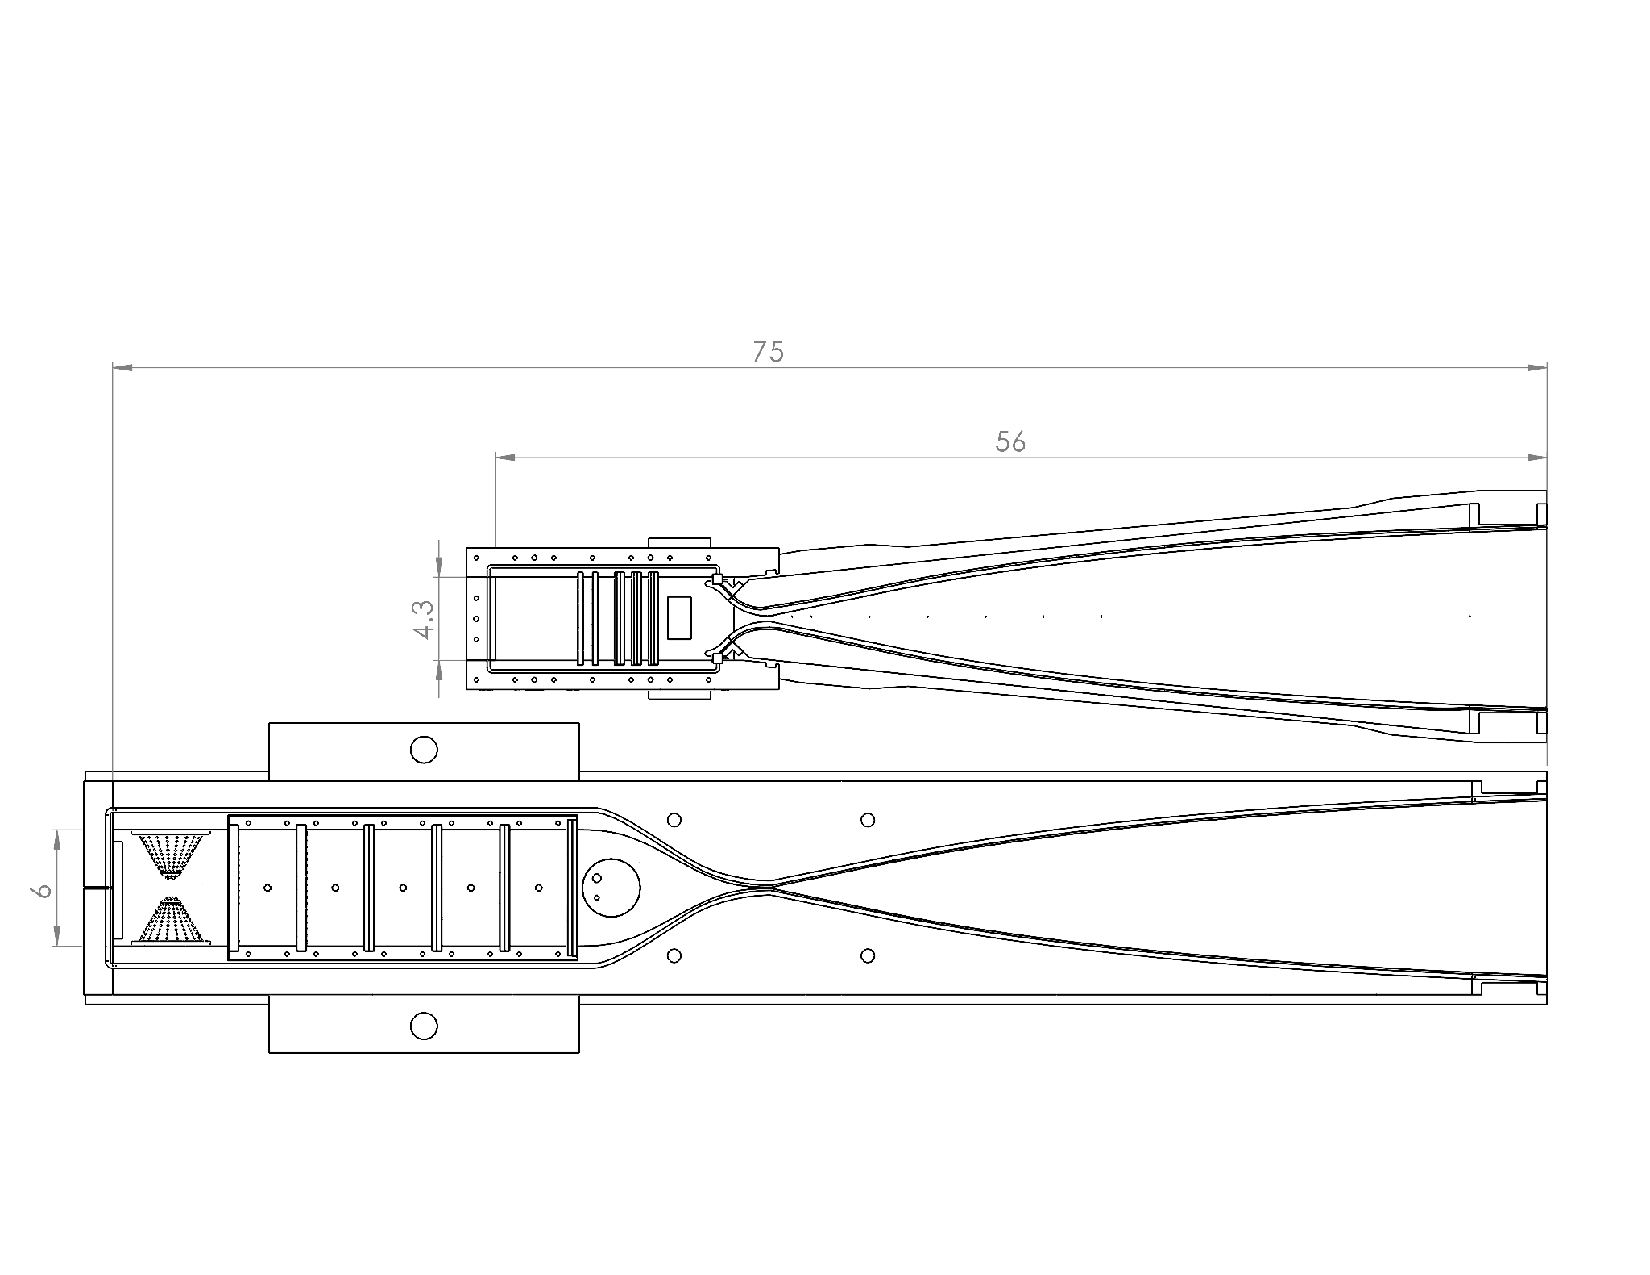
\includegraphics[trim={12 100 40 162},clip,width=6in]{nozzles.pdf}
    \caption{Comparison of ACE (top) and ACE2.0 (bottom) nozzle and settling chamber designs}
    \label{fig:nozzles}
\end{figure}

All of the nozzle and settling chamber parts will be made from 304 stainless steel except for the flexures, which will be made from Condition A 17-4 PH stainless steel for maximum strength while maintaining flexibility.

\subsection{Mechanical Design Iterations}

There were a few distinct iterations throughout the design process of ACE2.0 that are worth mentioning briefly. As mentioned, enabling active control was not the original intent of the ACE redesign, so the initial mechanical design was limited. One major difference to note between all of the past iterations and the final iteration is that the nozzle and settling chamber upper and lower pieces are not single rigid parts in the past iterations. The plan was to have either a bolted or welded interface between the nozzle blocks and the settling chamber piece to save cost in stock material, but it was decided to accept the higher cost of material for maximum strength and rigidity with a single piece.

A preface to the mechanical designs is that the actual load on the settling chamber and nozzle at a maximum pressure of 200 psia is around 90,000 pounds per top and bottom. This is the result of the increased surface area of the settling chamber and subsonic portion of the nozzle, which together is 14 inches wide by 36 inches long.

The first iteration, shown in Figure \ref{fig:i1}, had a system of worm gears and lead screws to simultaneously adjust both nozzle blocks, and it required a jam nut on each lead screw and large wedges on the settling chamber to lock the position during a run. This design was not intended to be active, so it could not dynamically support the loads during a run. This design revealed that active control was not far from reach, so the next iteration began with the intention to enable it.

\begin{figure}[ht!]
    \centering
    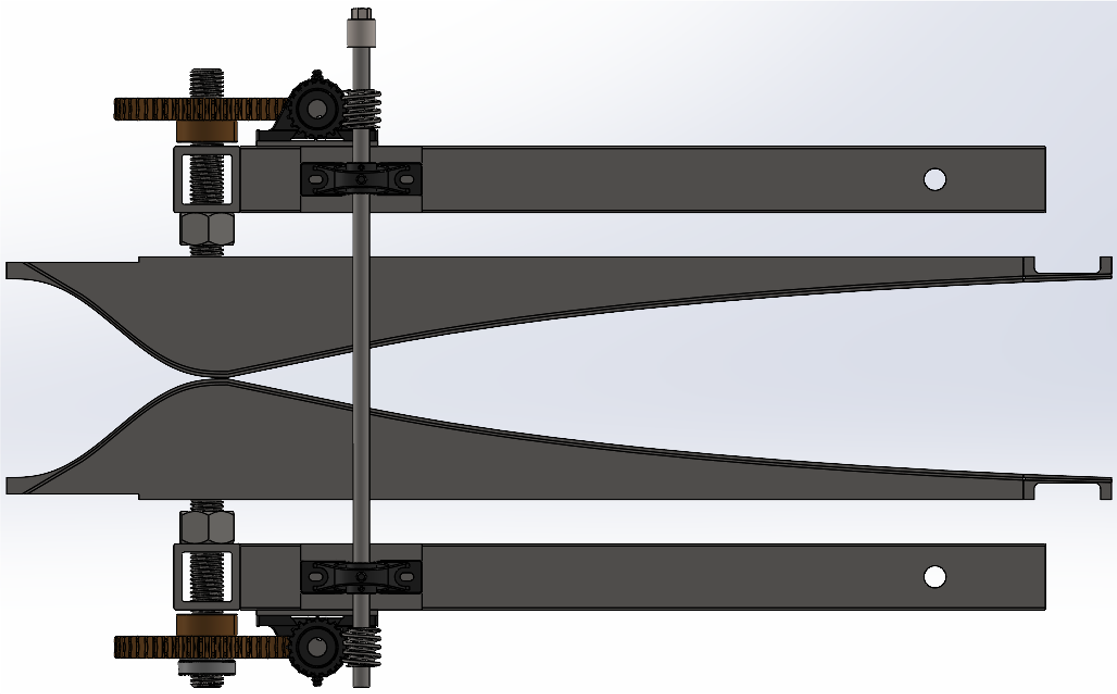
\includegraphics[width=5in]{i1a}
    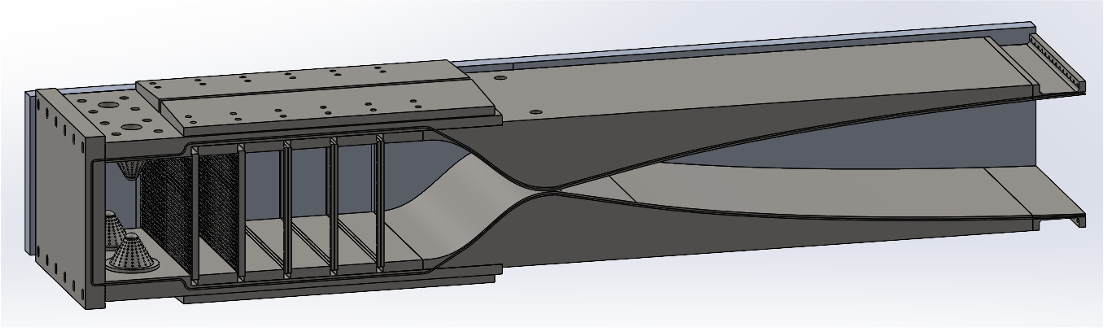
\includegraphics[width=5in]{i1b}
    \caption{Iteration 1 of ACE2.0: Non-active}
    \label{fig:i1}
\end{figure}

The second iteration, shown in Figure \ref{fig:i2}, built off from the idea of the wedges on the settling chamber to fully support against the loads during a run. This design relied on specially contoured oil-impregnated bronze sliding plates that were actuated by a similar system of worm gears and lead screws. The purpose of the contours instead of a simple flat wedge was to (1) provide a constant rate of change for the Mach number given a constant lead screw translation rate input and (2) maintain all points of contact as the nozzle rotated. The primary concern with this design was the expected wear and required actuation force due to friction, which would be around 20,000 pounds assuming a friction coefficient of 0.2 between the stainless steel and oil-impregnated bronze. This design also had the introduction of the disc spring stacks at the settling chamber end to hold the nozzles apart at the set position while not under load. 

\begin{figure}[ht!]
    \centering
    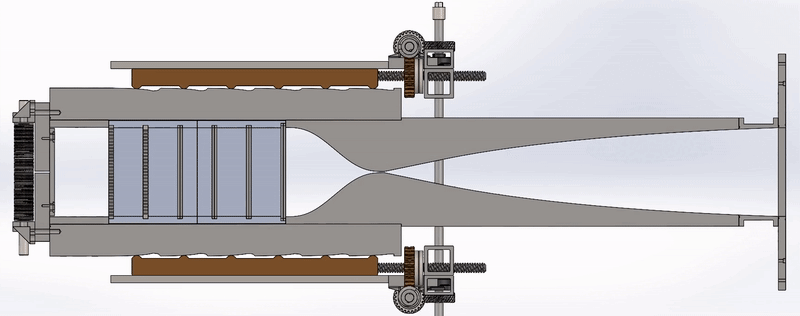
\includegraphics[width=6in]{i2}
    \caption{Iteration 2 of ACE2.0: Sliding Wedge}
    \label{fig:i2}
\end{figure}

The third iteration, shown in Figure \ref{fig:i3}, improved upon the previous approach by introducing rollers and bearings to eliminate the friction and linear actuators for simpler and more robust control. This design was abandoned for two primary reasons: (1) a realization that the reverse load while under full vacuum was unsupported and (2) feedback from machinists about concerns of wear in bearings and difficulty in machining the roller plate. The load under full vacuum across the entire nozzle and settling chamber is around 16,000 pounds, which requires substantial support to maintain the set Mach number when initiating a run and to minimize excess loads on the flexure.

\begin{figure}[ht!]
    \centering
    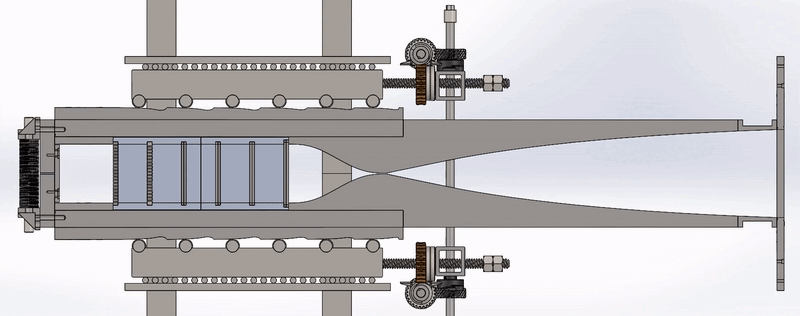
\includegraphics[width=6in]{i3}
    \caption{Iteration 3 of ACE2.0: Rollers and Actuators}
    \label{fig:i3}
\end{figure}

The fourth and final iteration turned to a complete different approach of using 20-ton ball screw linear actuators to fully support both the maximum pressure and full vacuum loads. This final iteration is the most simple mechanically while also providing the most versatility in controlling the Mach number.

\subsection{20-Ton Linear Actuators Design}

The final design of ACE2.0 utilizes two 20-ton ball screw linear actuators on both the upper and lower nozzle blocks to actively control the Mach number by varying the throat height. The final design of the nozzle and settling chamber with the actuators can be seen in Figure \ref{fig:cad-nozzle-actuators}. 

\begin{figure}[ht!]
    \centering
    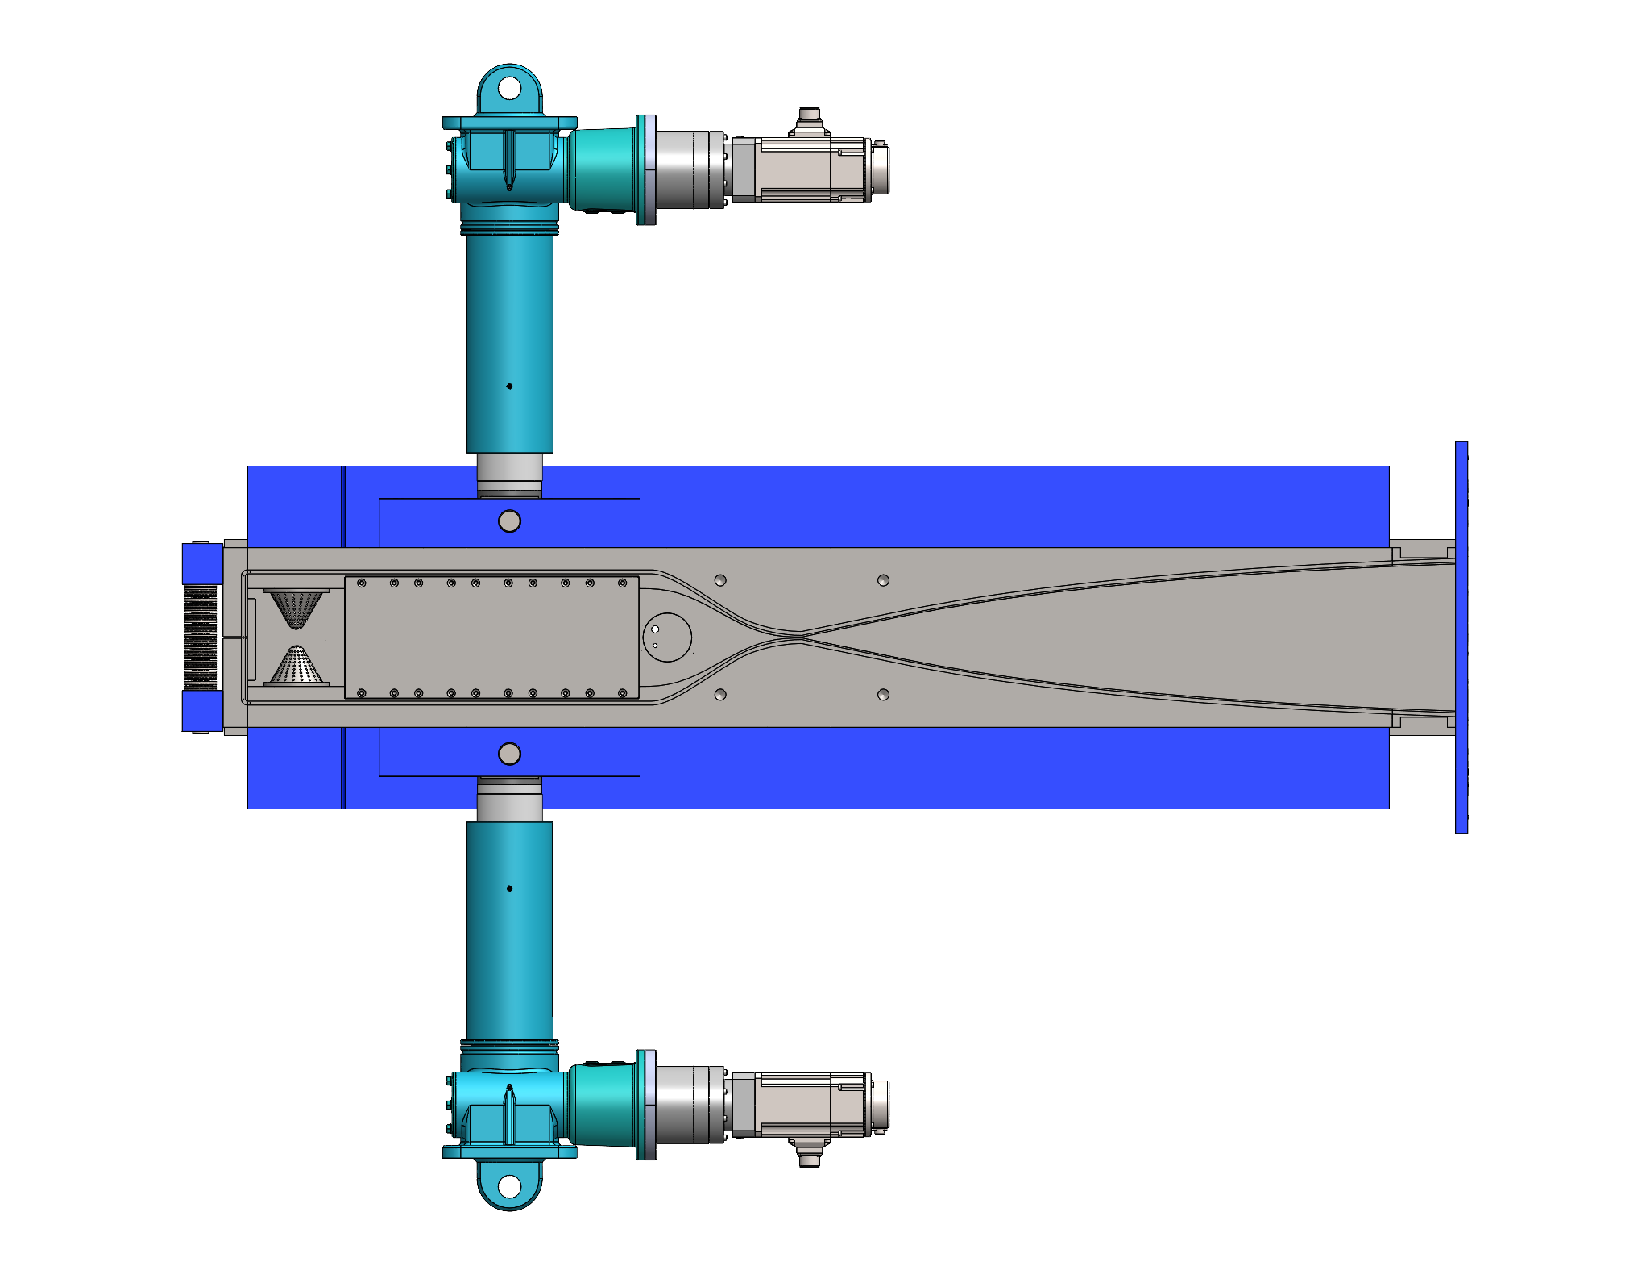
\includegraphics[trim={80 30 80 30},clip,width=5in]{cad-nozzle-actuators.pdf}
    \caption{ACE2.0 final nozzle and settling chamber with actuators}
    \label{fig:cad-nozzle-actuators}
\end{figure}

\subsubsection*{Nozzle and Settling Chamber Design}

Using linear actuators does present the challenges of introducing stress concentrations at the attachment location and not providing support along the length of the nozzle and settling chamber. These were overcome by making the mating clevis on the settling chamber a 16 inch bar to distribute the load and adding a 5 inch by 2.5 inch beam along the length of the nozzle and settling chamber to provide rigidity, as seen in Figure \ref{fig:cad-nozzle-actuators}.

The sidewalls are 1.5 inches thick and made from 304 stainless steel. They are suspended from the frame by two brackets each, and a series of custom bar clamps will provide the support against the load under pressure. One sidewall has all of the ports and sensors, which allows the other to be the main access for maintenance.

The settling chamber consists of four inlet flow spreading cones and a standalone box where the flow conditioners enclosed that allows for easy maintenance and future modifications of screen configurations. The inlet flow spreading cones were added to allow uniform mixing of the incoming air before flowing through the aerogrids, and they will be made from 304 stainless steel. The flow conditioner box is made from four 0.75-inch thick 304 stainless steel plates. This assembly floats between the nozzles and is secured by the sidewalls in a slot. The overall height doubles as a safety limit so the nozzles will contact each side of the box before contacting each other. Housed inside the box are two aerogrids and four screens in the current configuration, but any configuration can easily be designed and swapped in the future. The initial configuration provides 3 inches between each aerogrid and screen for adequate turbulence decay. The flow conditioner box is shown in Figure \ref{fig:conditioners}. 

The aerogrids are made from 0.5-inch thick 304 stainless steel. As shown in Figure \ref{fig:aerogrid}, they each have around 2750 0.125-inch diameter holes for an open area of 40\%. The resulting maximum pressure drop across each aerogrid is approximately 18 times the dynamic pressure, which is 0.3 psia at a 200 psia inlet stagnation pressure. The initial choices of wire mesh for the screens will be explored prior to installation. The first screen will likely have a wire diameter of 0.0035 inches, an opening size of 0.0085 inches, and an open area of 50\%. The last screen will likely have a wire diameter of 0.0023 inches, an opening size of 0.0033 inches, and an open area of 34\%. The maximum pressure drop across these screens will be approximately 5 and 15 times the dynamic pressure, respectively. 

The variable flow conditioner box will allow future optimization for the best incoming flow quality. The objective in this work is to maintain the flow quality of ACE, so some optimization of the flow conditioners will be performed depending on results during the characterization of ACE2.0.

\begin{figure}[ht!]
    \centering
    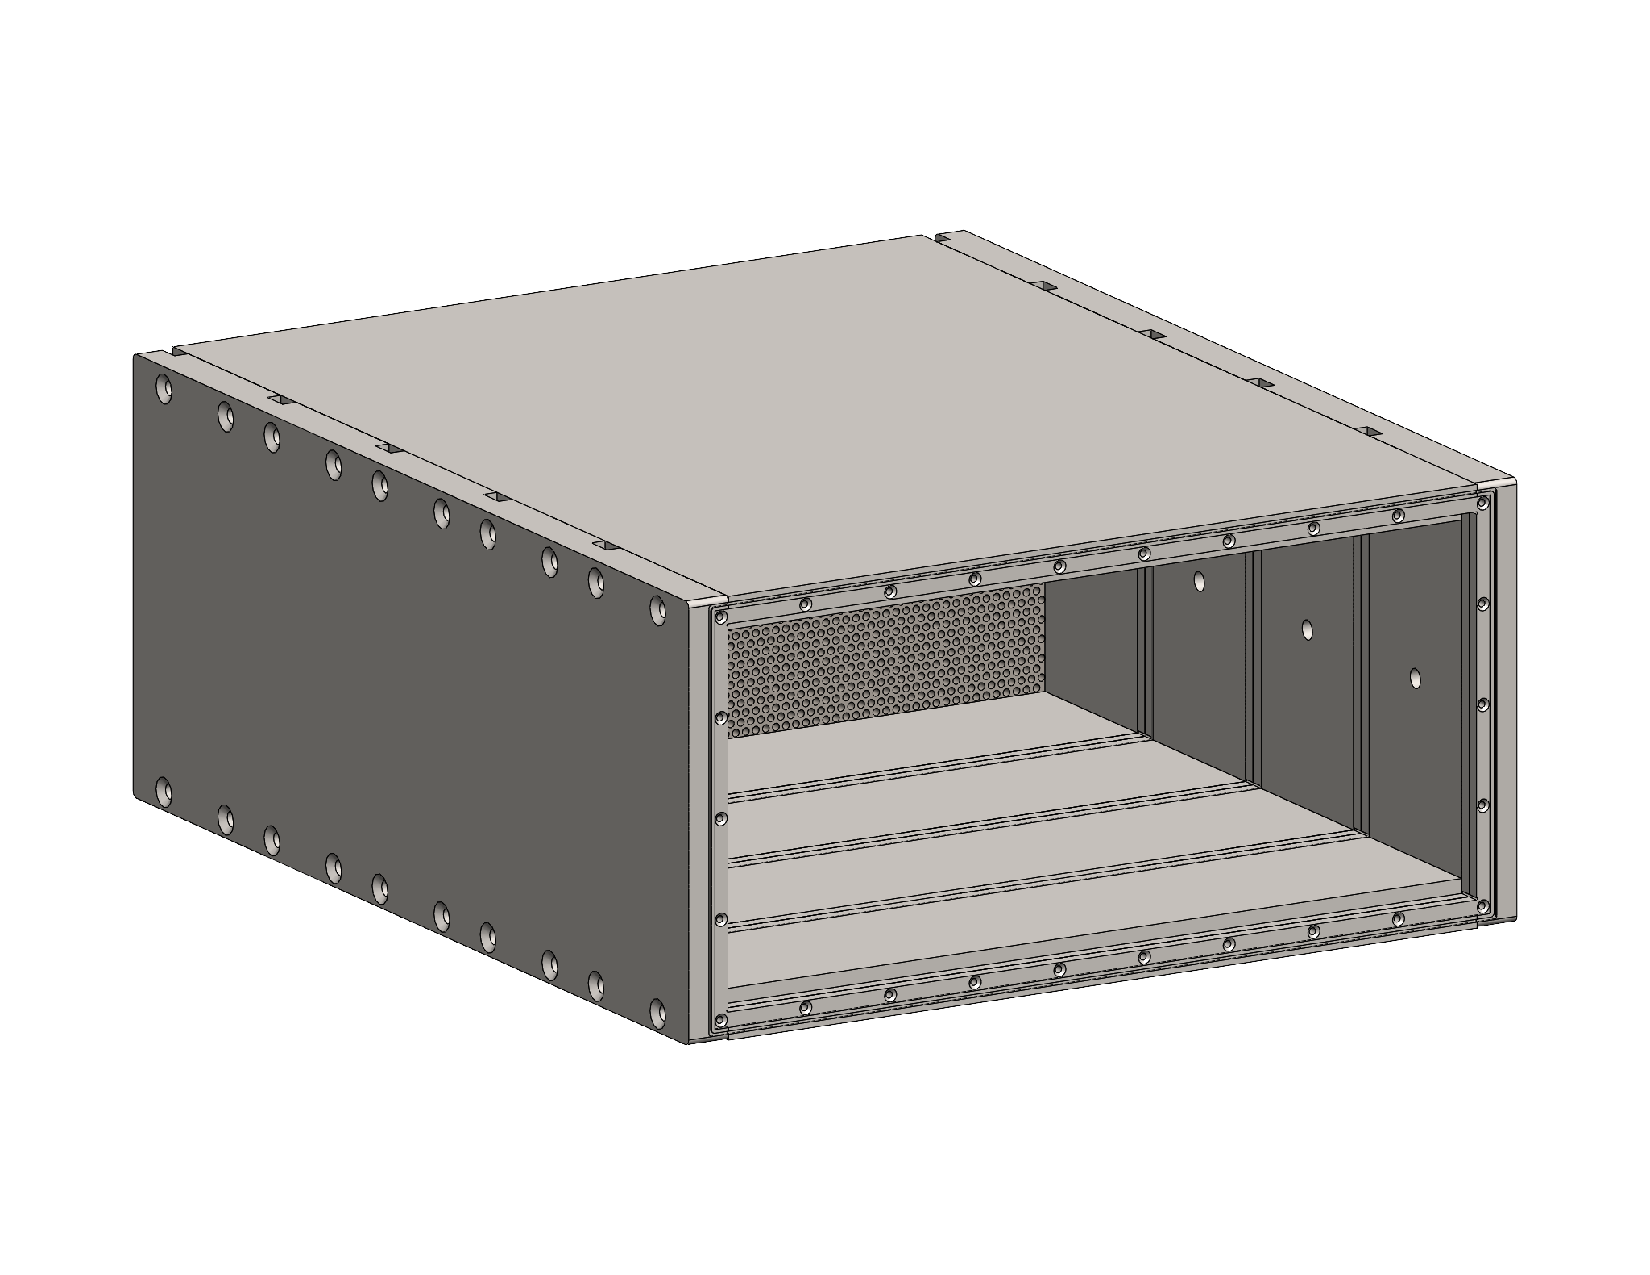
\includegraphics[trim={50 80 50 80},clip,width=5.5in]{conditioners.pdf}
    \caption{CAD model of flow conditioner box}
    \label{fig:conditioners}
\end{figure}

\begin{figure}[ht!]
    \centering
    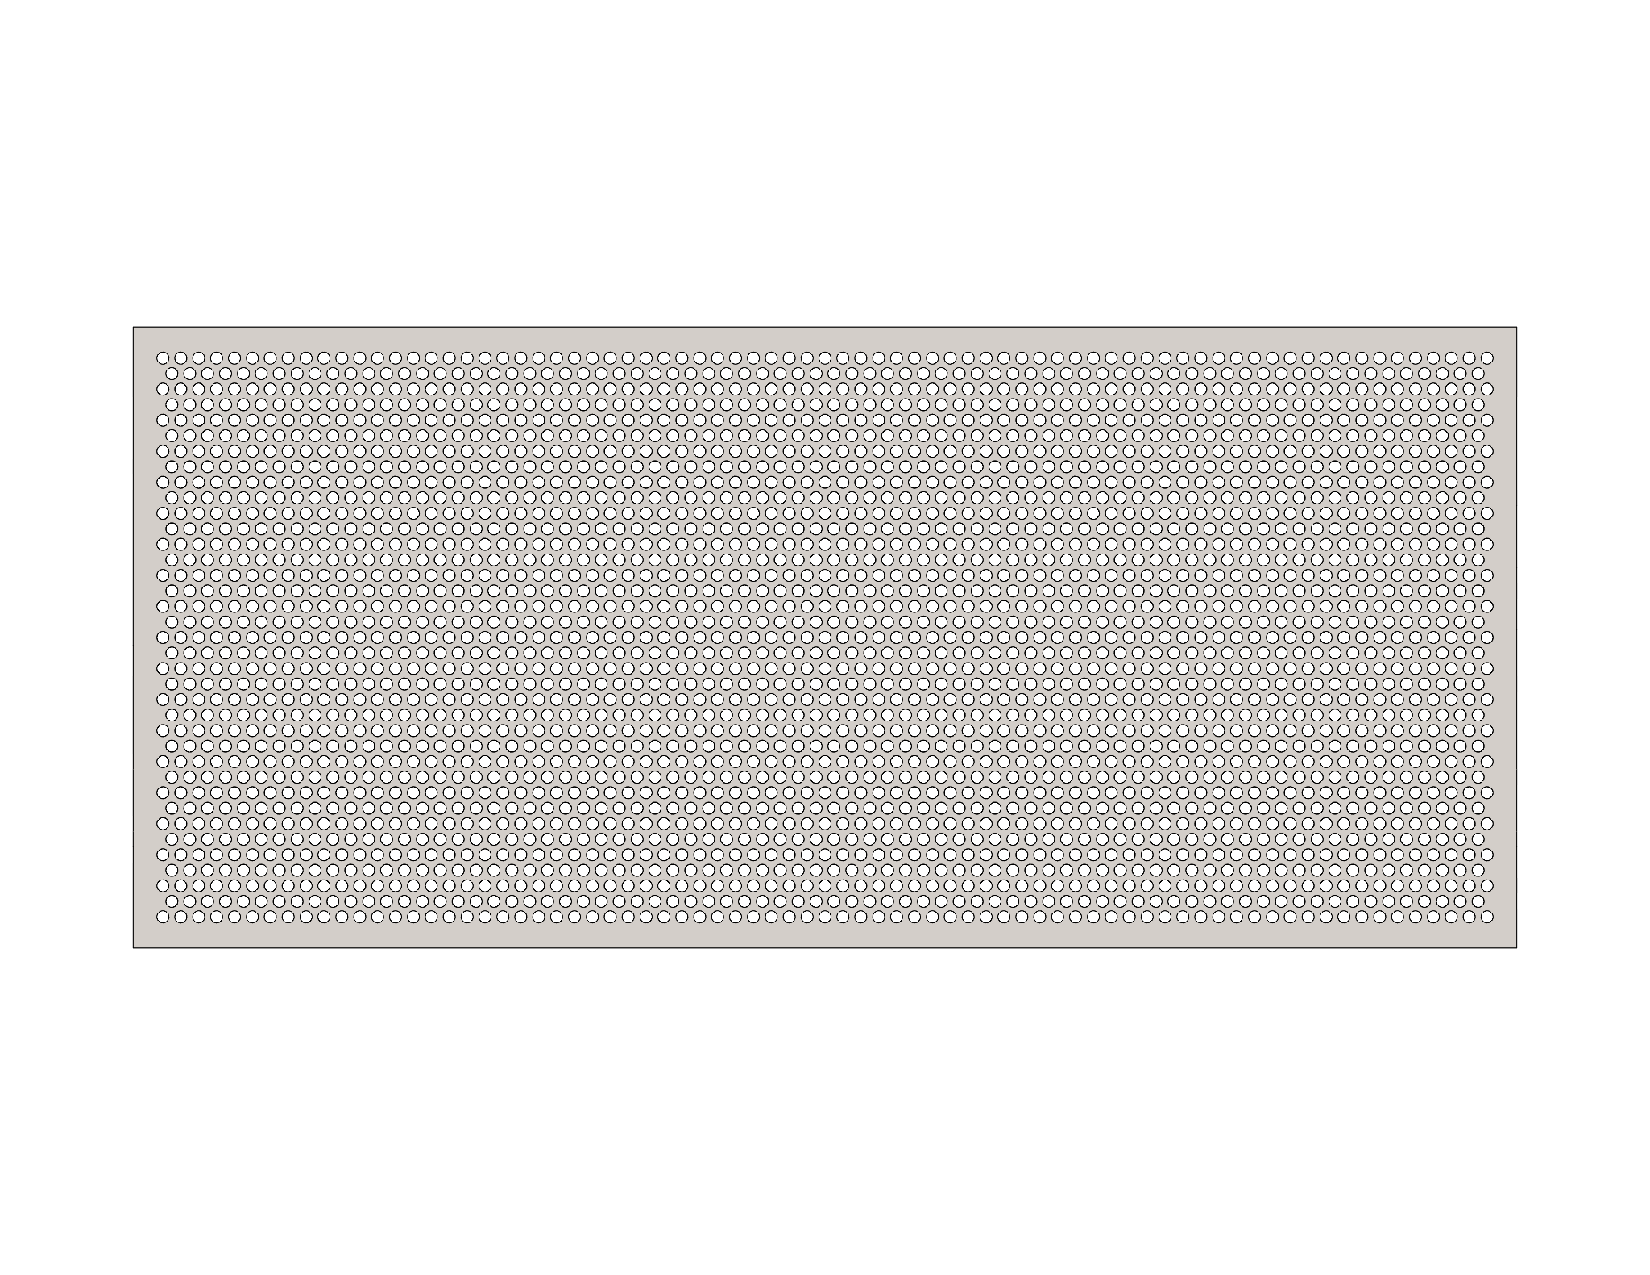
\includegraphics[trim={50 150 50 150},clip,width=5.5in]{aerogrid.pdf}
    \caption{CAD model of aerogrid}
    \label{fig:aerogrid}
\end{figure}

\subsubsection*{Frame Design}

The frame was designed around the linear actuators to best support the extreme loads. In order to maximize strength, a single piece brace was designed to symmetrically bear the loads from the actuators. The rest of the frame was designed between the brace and the nozzle-test-section flange to support the sidewalls. The entire frame will be made from 3 inch thick 4140 alloy steel plates and bars, and it all bolts together instead of welding. All exposed faces will be powder coated in order avoid rust and wear over time. 

The frame will have four 5000-pound capacity steel swivel casters for easy maneuvering when aligning for installation. Once in position, the weight of the assembly will be transferred to rigid feet on threaded rods. All of these details can be seen in Figure \ref{fig:cad-frame}.

\begin{figure}[ht!]
    \centering
    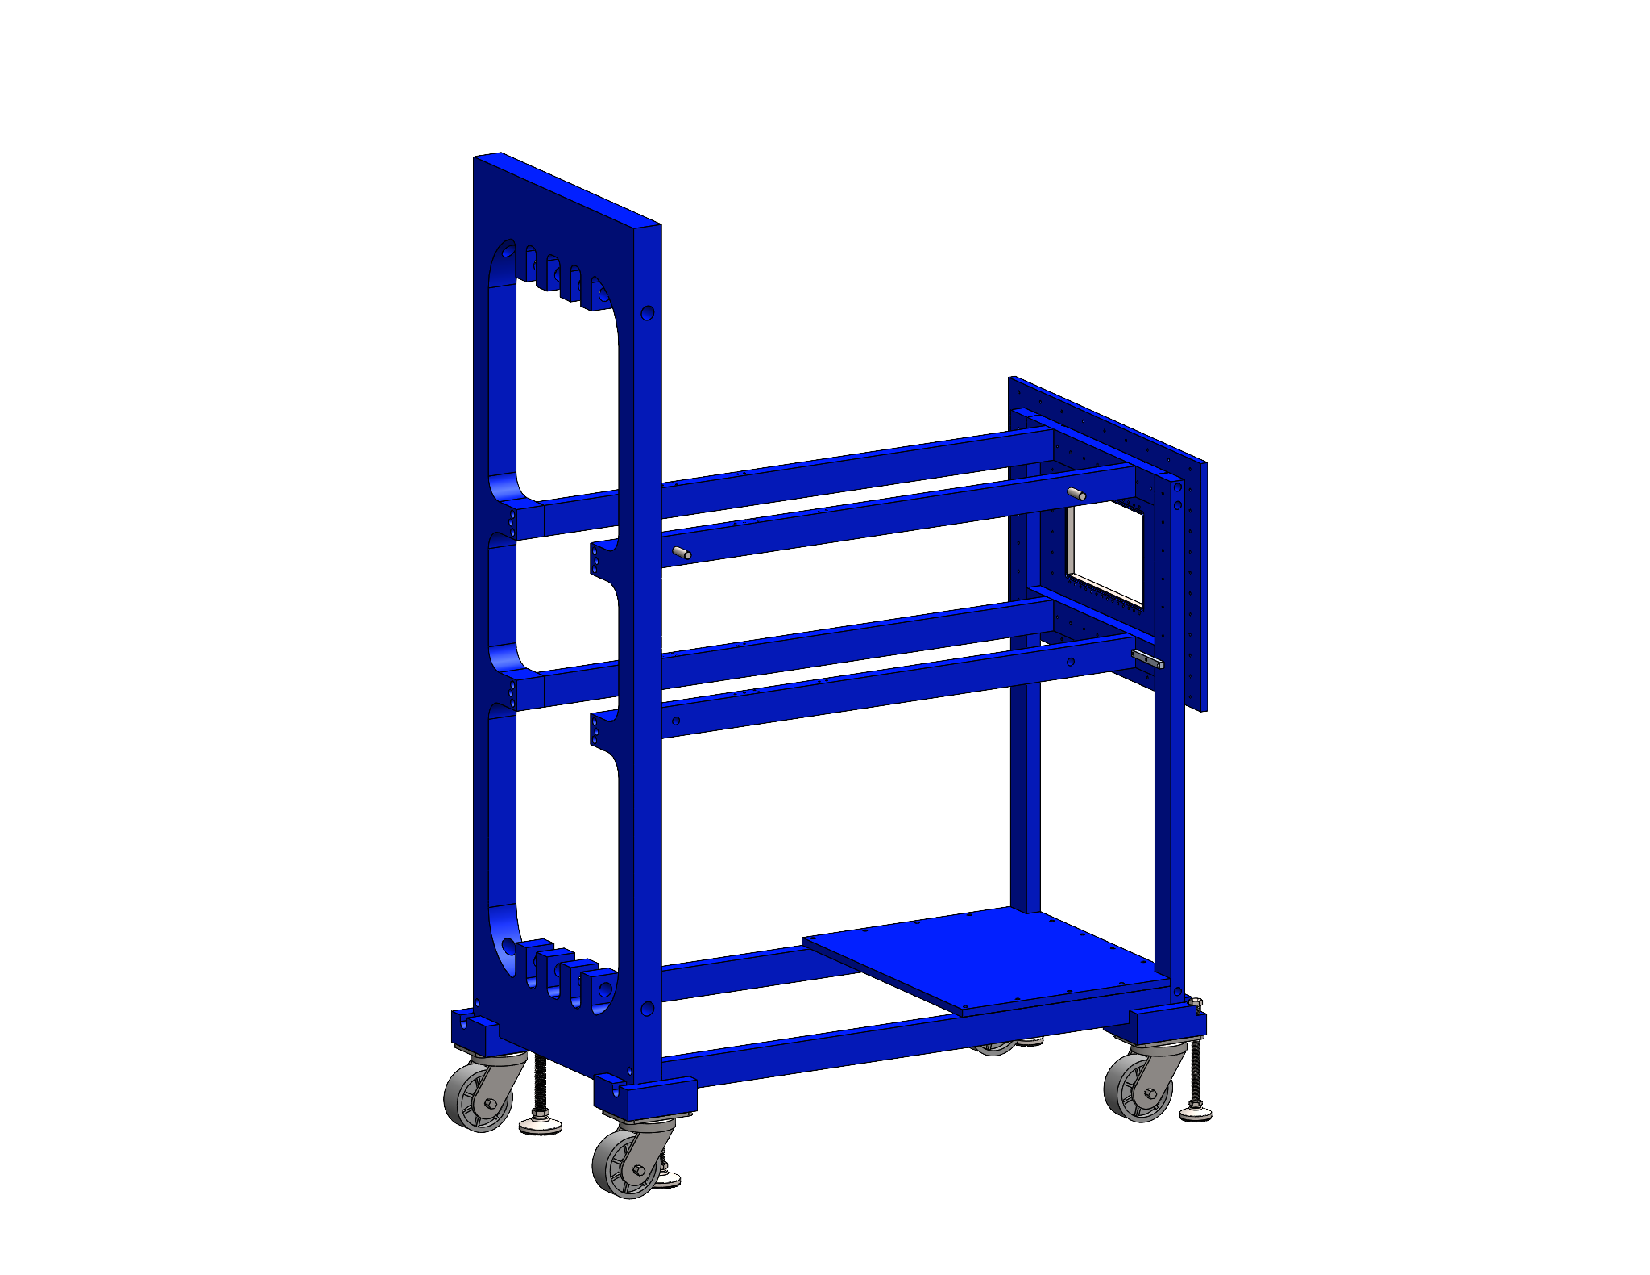
\includegraphics[trim={160 30 160 70},clip,width=5in]{cad-frame.pdf}
    \caption{CAD model of full frame assembly}
    \label{fig:cad-frame}
\end{figure}

\subsubsection*{Actuation System Design}

The actuation system for ACE2.0 is comprised of many components that enable the active  feedback-back control of the Mach number. Only a high level overview will be provided here for sake of brevity, but a full detailed description of the entire system will be provided in a future appendix.
%Appendix \ref{appendix:actuation}. 

The linear actuators are each rated for 40,000 pounds with a minimum FOS of 7. They have a double clevis design to rotate freely and have a custom motor mount for the selected gear box and servo motor, as shown in Figure \ref{fig:actuators}. The actuators are comprised of a 24:1 worm gear reducer that turns a ball nut to drive a 0.5 inch lead ball screw. The ball nut has a long service life that will allow over 400,000 full throat deflections before maintenance is required. Another 20:1 gear box will be mounted to each actuator for an overall travel of approximately 0.001 inch per servo motor turn.

\begin{figure}[ht]
    \centering
    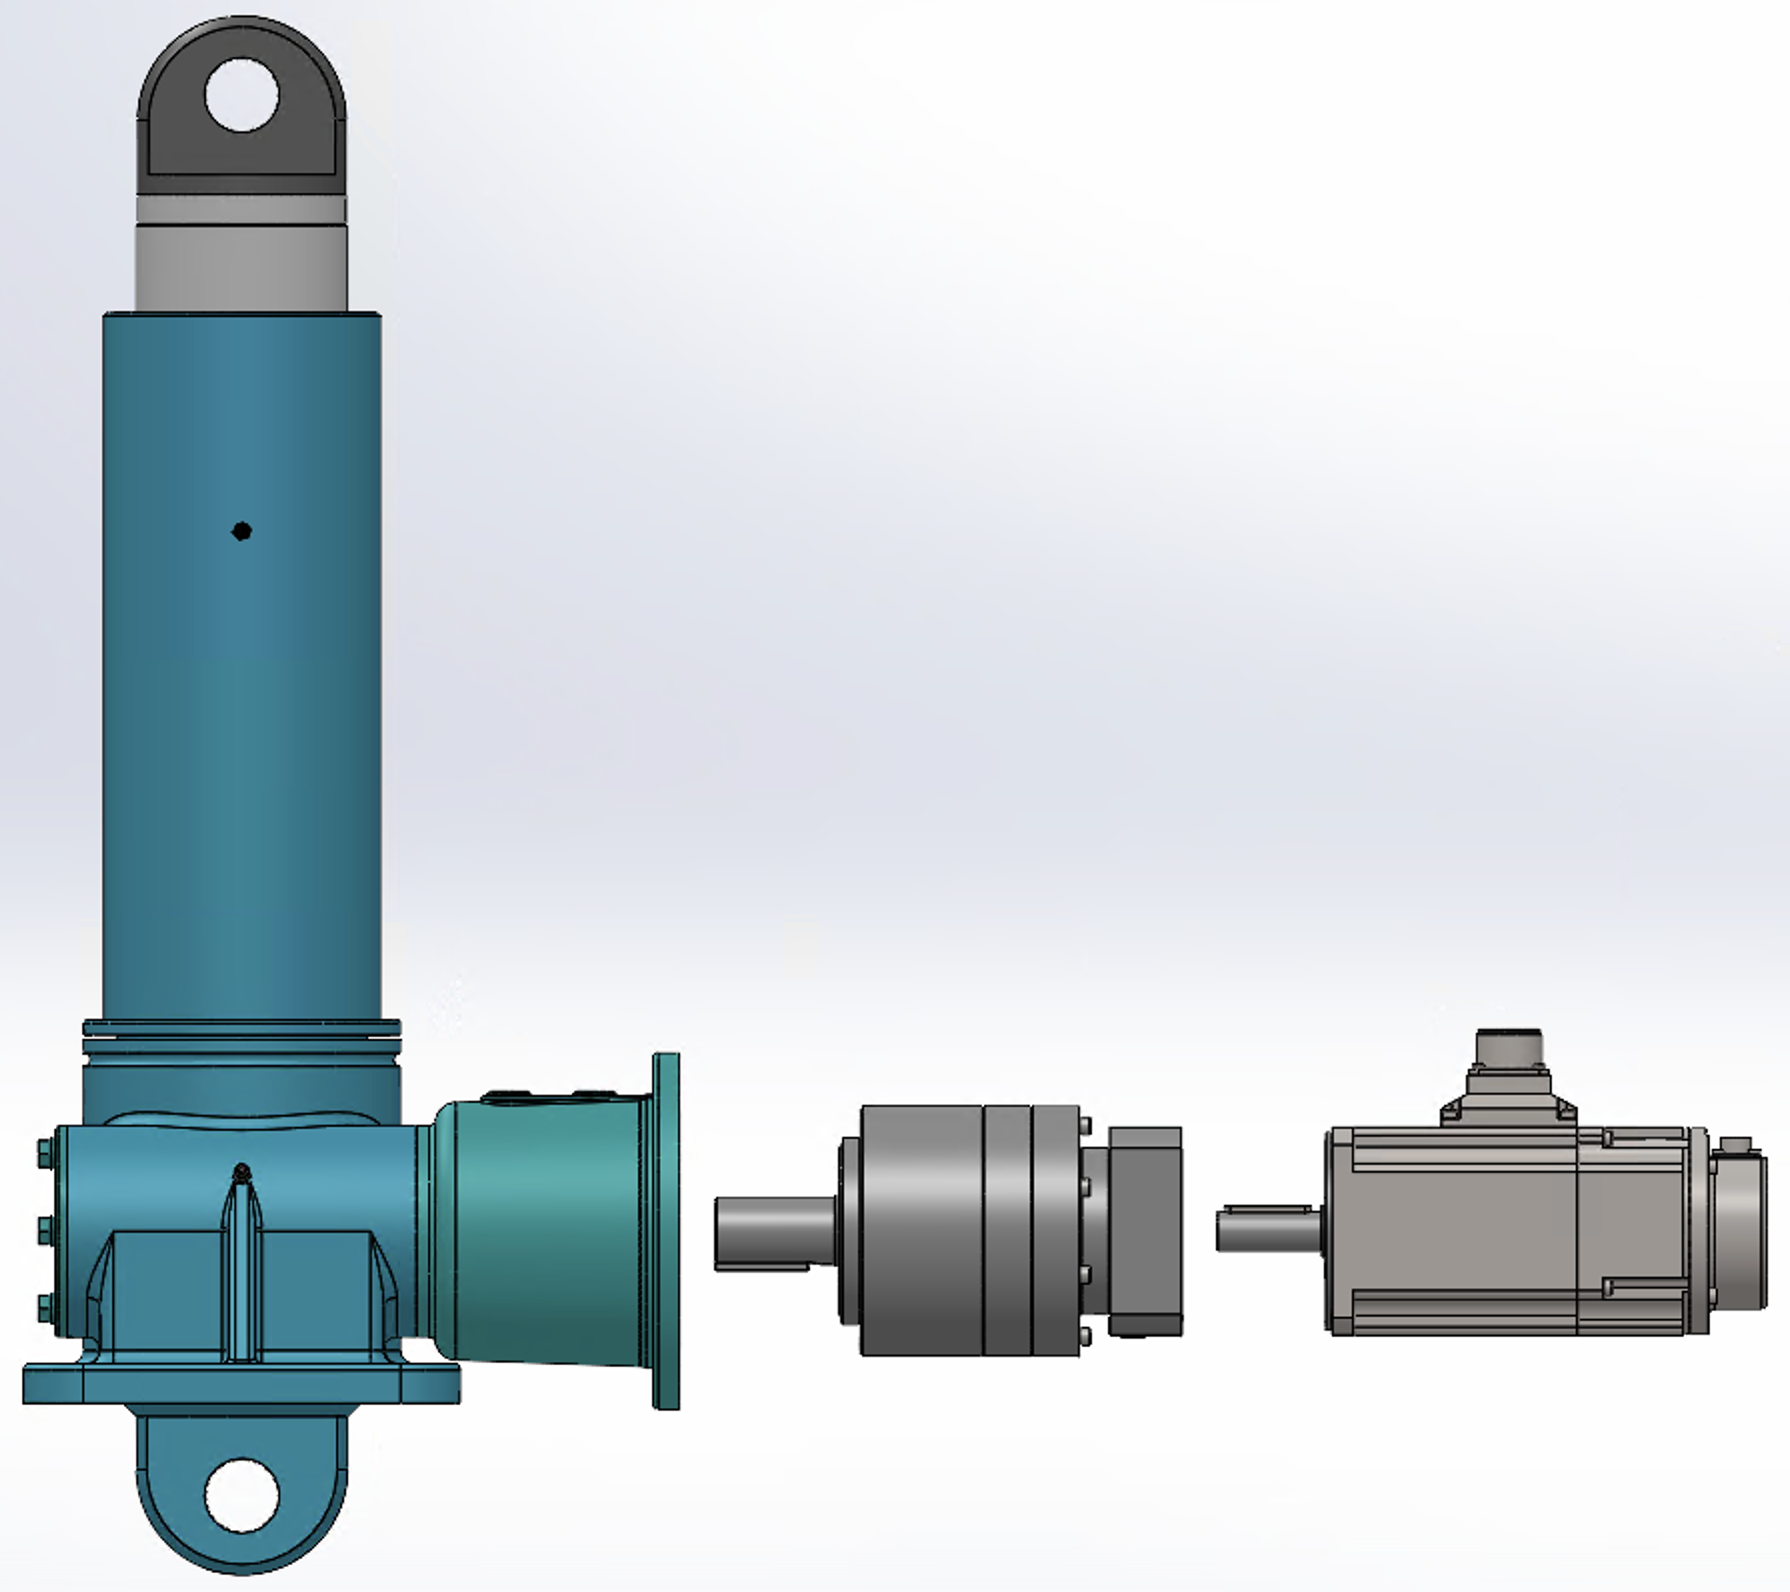
\includegraphics[width=5in]{actuators}
    \caption{CAD model of 20-ton linear actuator, 20:1 gear box, and servo motor.}
    \label{fig:actuators}
\end{figure}

The required input torque for the actuators at maximum load with the additional gearbox is 28 inch-pounds. The rated continuous torque and the momentary peak torque of the selected servo motor are 28 and 84 inch-pounds, respectively, and the rated continuous speed and the momentary peak speed are 3000 and 5000 revolutions per minute, respectively. The change in throat height from Mach 5 to 8 for each half of the nozzle is around 0.157 inches, so a full Mach sweep at maximum pressure can be achieved in around 3 seconds within the continuous operation range of the servo motor. The servo motors have a power-off brake hold a set Mach number and to prevent motion and any potential damage in a power outage.

In order to minimize the backlash in the actuators, two inverted stacks of Belleville disc springs were added to the end of the settling chamber as shown in Figure \ref{fig:springs}. With a nominally linear relationship between force and compression, a stack height of 8 inches and minimum compression of 0.875 inches was chosen to produce a combined minimum force of 3000 pounds to always lift the upper nozzle block and keep the actuators in compression.

\begin{figure}[ht!]
    \centering
    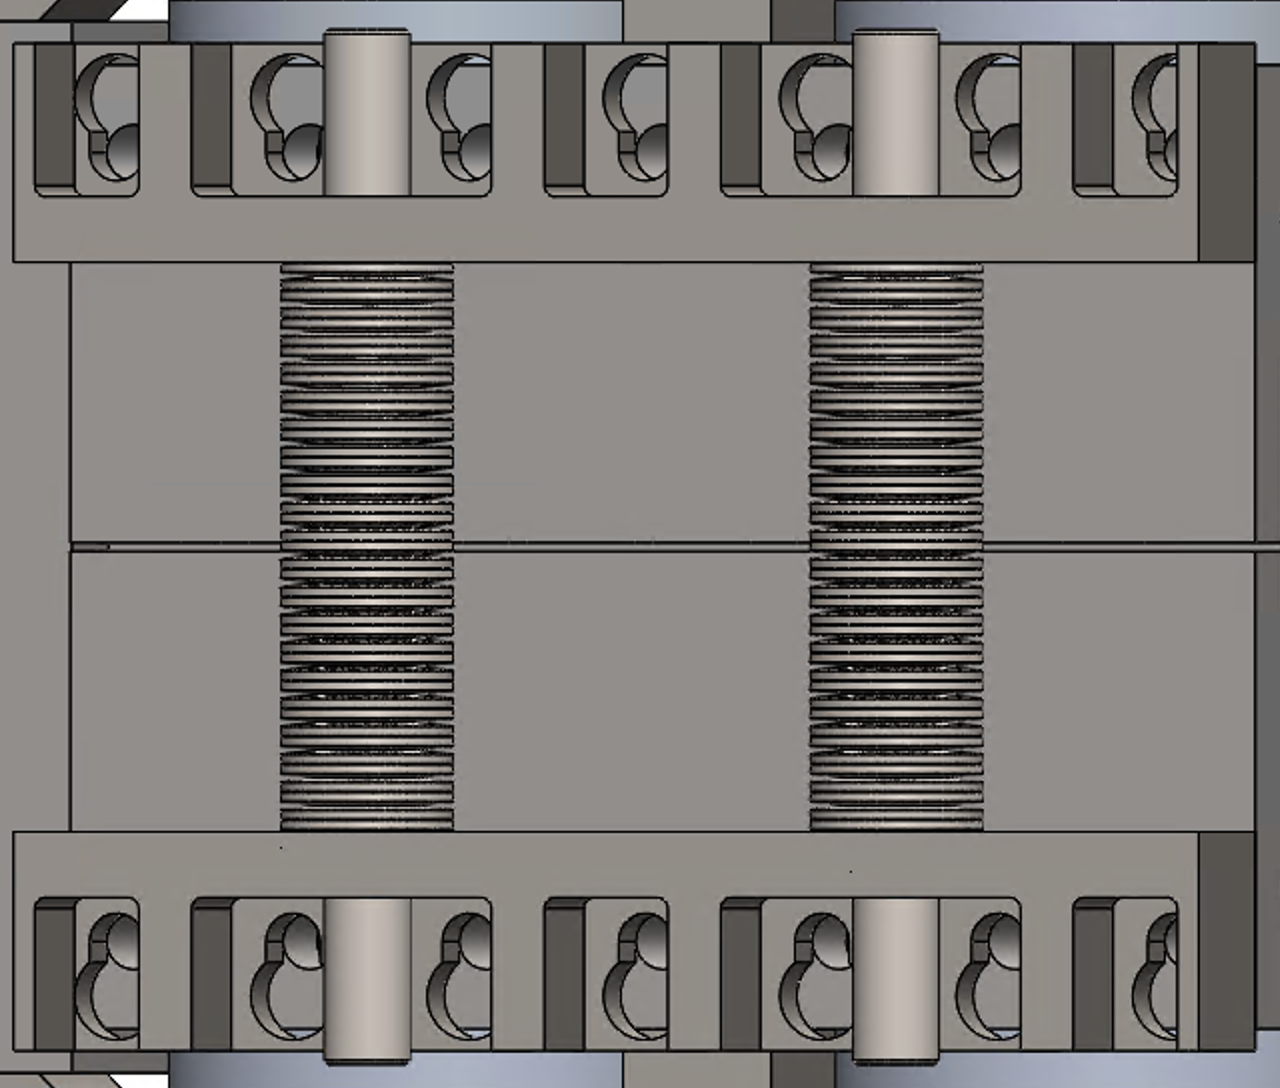
\includegraphics[width=5in]{springs}
    \caption{Inverted disc springs stacks at the end of the settling chamber}
    \label{fig:springs}
\end{figure}

The four servo motors are each driven by individual servo drives powered by 240 VAC 3-phase. These four drives and servo motors are controlled synchronously by a programmable logic controller (PLC) through EtherCAT, the fastest industrial Ethernet communication protocol. The PLC logic programs are written its associated software, Sysmac Studio. This software is a graphical ladder logic environment designed to integrate many automation devices across EtherCAT.

The specific program to control the Mach number will be created in future work. This program will initially be designed with four control objectives: (1) precise set Mach number, (2) Mach number sweep with specified start, stop, and time, (3) Mach number schedule, and (4) feedback-control for Mach number. The completed Mach number control program will be provided in a future appendix.
%Appendix \ref{appendix:actuation}. 
Additionally, three analog modules were added to the PLC to input the static pressure, stagnation pressure, and temperature measured by the corresponding sensors to enable feedback-control. 

Additional components of the system include two safety limit switches for each actuator, an external encoder for each actuator for additional physical feedback, various power supplies and relays, an emergency stop button, and a 7" human machine interface (HMI) for a simple control interface that can be updated and expanded for any desired controls.

\subsubsection*{Final Overall Design}

The final design with all modeled components is shown in Figures \ref{fig:cad-side} and \ref{fig:cad-full}. The entire design will integrate with the existing ACE test section and other infrastructure. The overall length from the nozzle-test-section flange to the inlet of the 4-way manifold is 94 inches, about 12 inches longer than the existing system.

\begin{figure}[ht!]
    \centering
    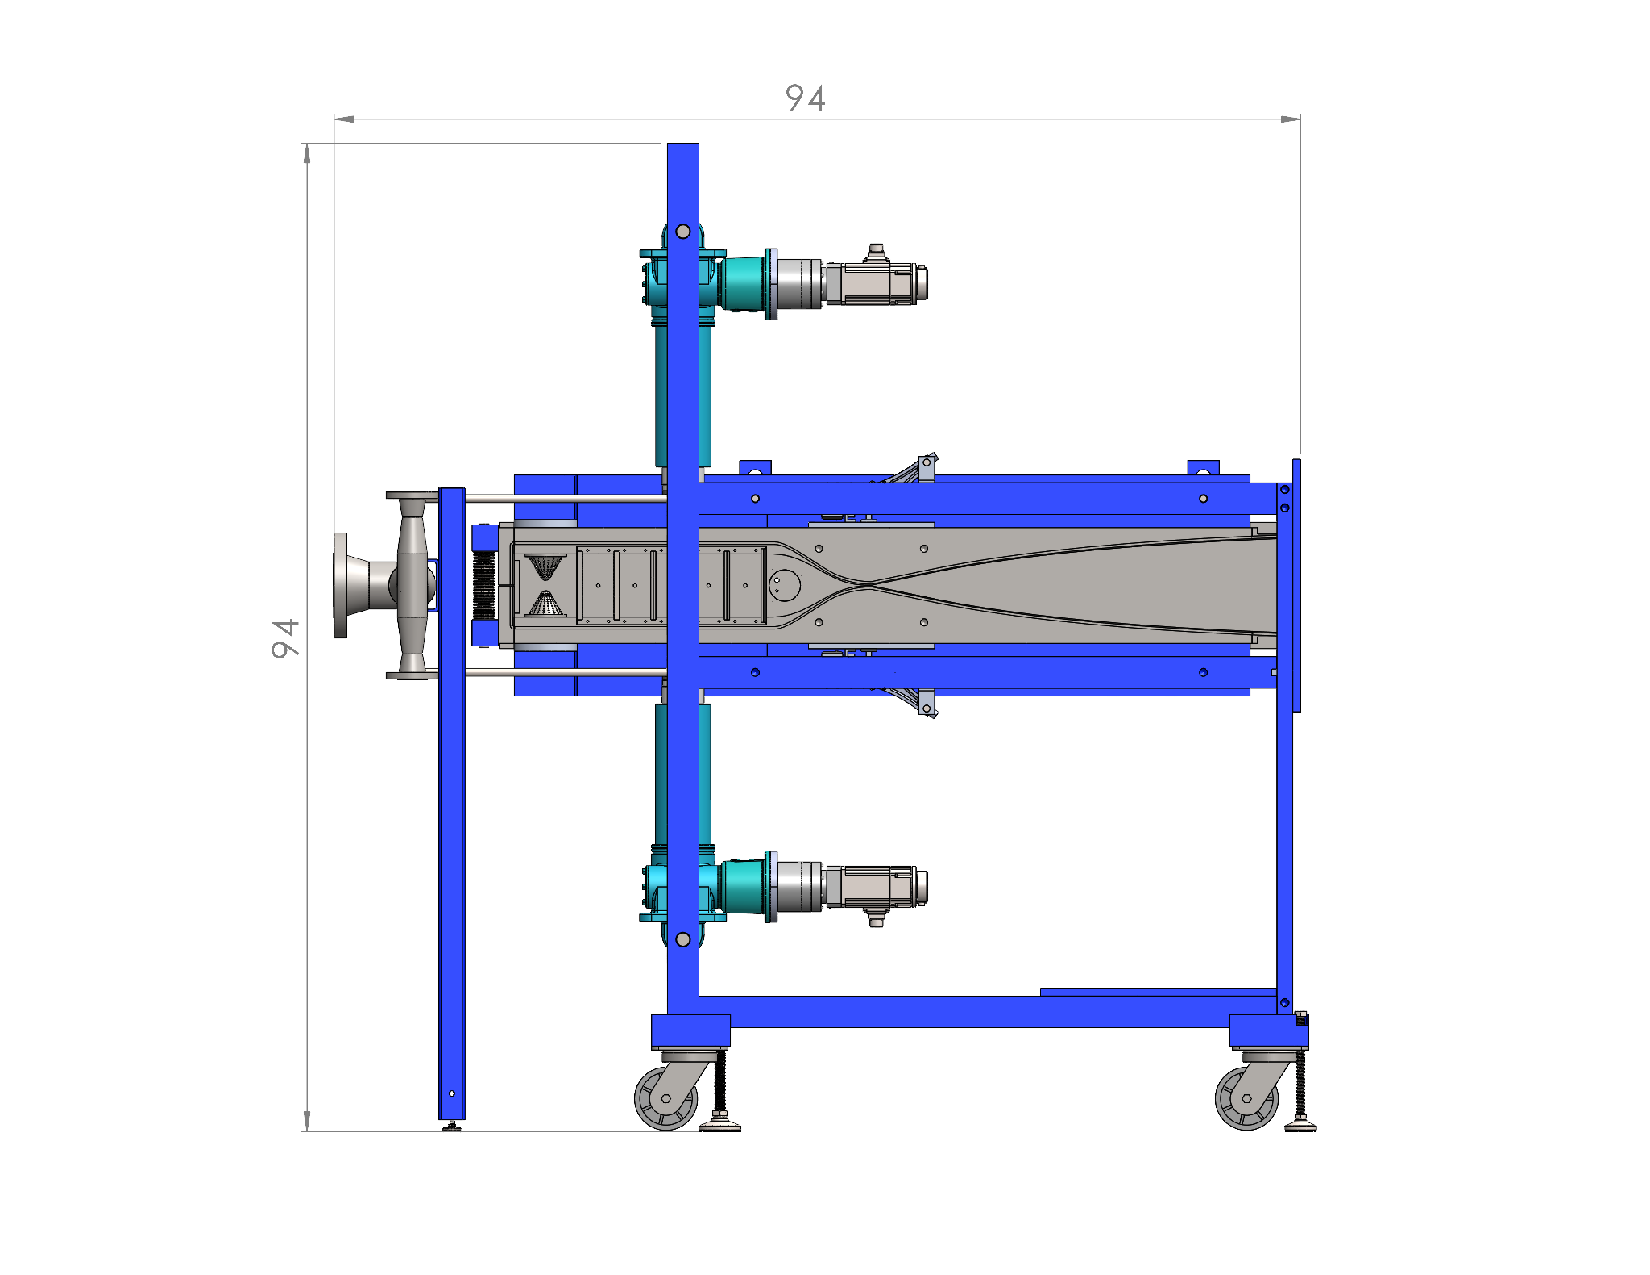
\includegraphics[trim={130 50 150 30},clip,width=6in]{cad-side.pdf}
    \caption{Side view of ACE2.0 in Solidworks}
    \label{fig:cad-side}
\end{figure}

\begin{figure}[ht!]
    \centering
    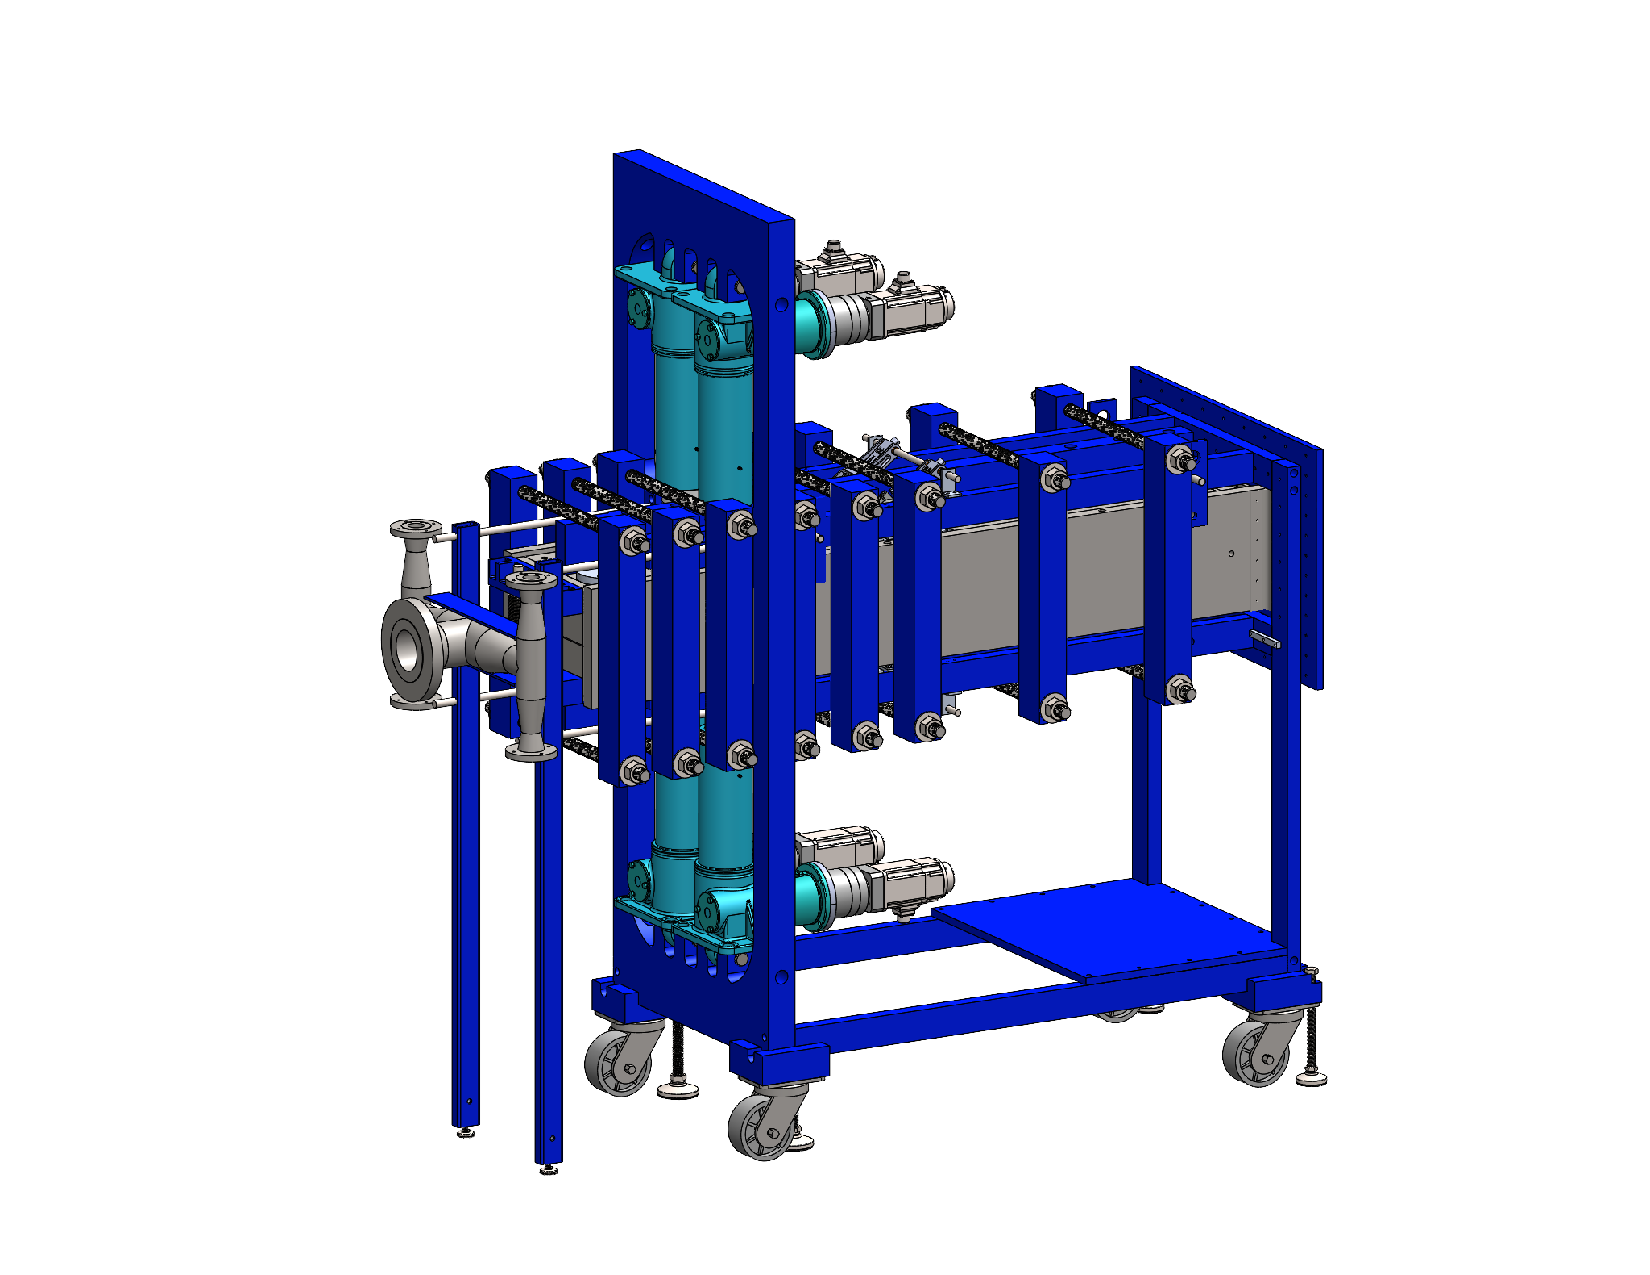
\includegraphics[trim={180 30 135 70},clip,width=6in]{cad-full.pdf}
    \caption{Full CAD model of ACE2.0 in Solidworks}
    \label{fig:cad-full}
\end{figure}

\clearpage

\subsubsection*{FEA}

The structural integrity of the final design was simulated using finite element analysis (FEA) in Solidworks. There were four primary simulations conducted: (1) lower nozzle and settling chamber at 200 psia with gravity, (2) upper nozzle and settling chamber at full vacuum with gravity, (3) sidewall with clamps at 200 psia, (4) and flexure fatigue at maximum deflection. Other simulations were also conducted for a many of the individual components such as the flow spreaders, aerogrids, and various hardware.

From all of these simulations, the minimum FOS for any component was 1.8. The displacement of the nozzle due to maximum load is shown in Figure \ref{fig:fea-full}. The maximum stress in the flexure shown in Figure \ref{fig:fea-flexure} is much less than the fatigue limit of 17-4 PH stainless steel.

\begin{figure}[ht!]
    \centering
    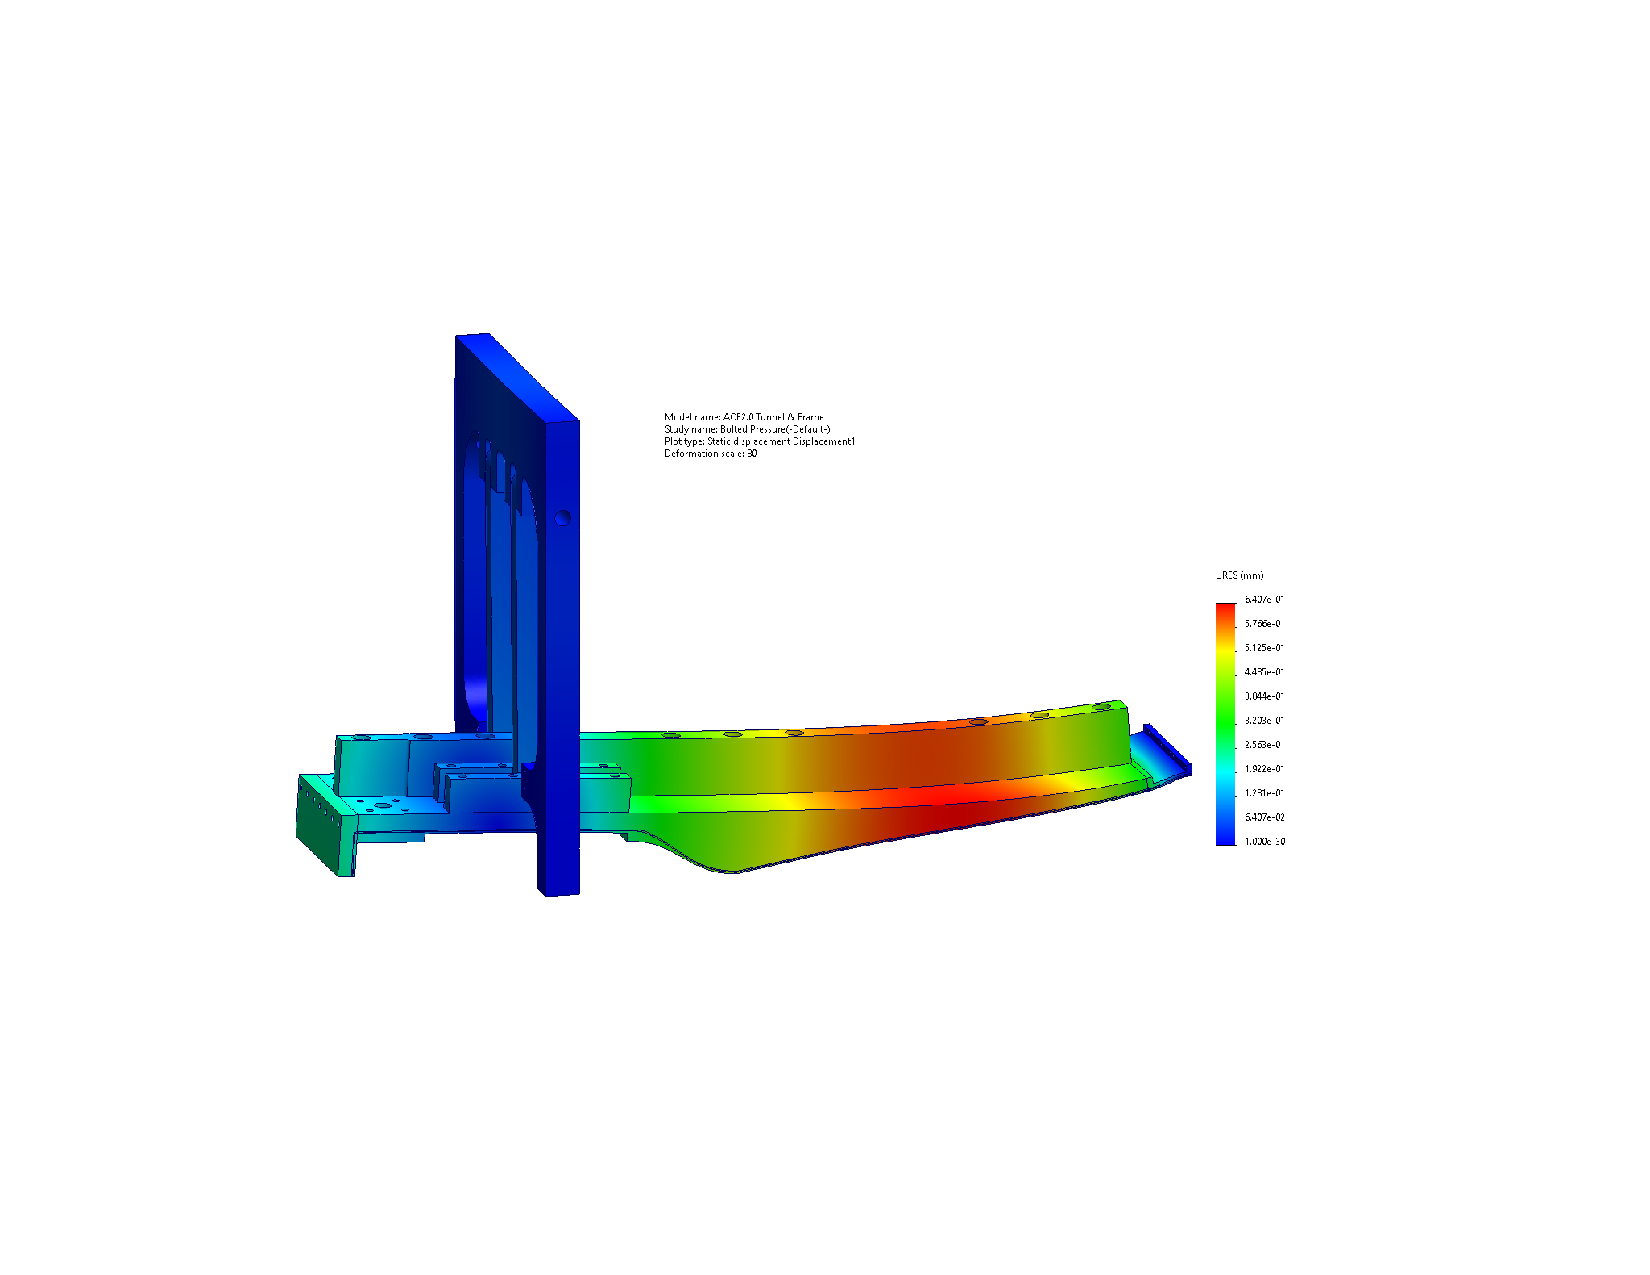
\includegraphics[trim={140 150 150 150},clip,width=6in]{fea-full.pdf}
    \caption{Displacement with 200 psia in settling chamber, 15 psia on exterior, gravity acting up, and bolted interfaces}
    \label{fig:fea-full}
\end{figure}

\begin{figure}[ht!]
    \centering
    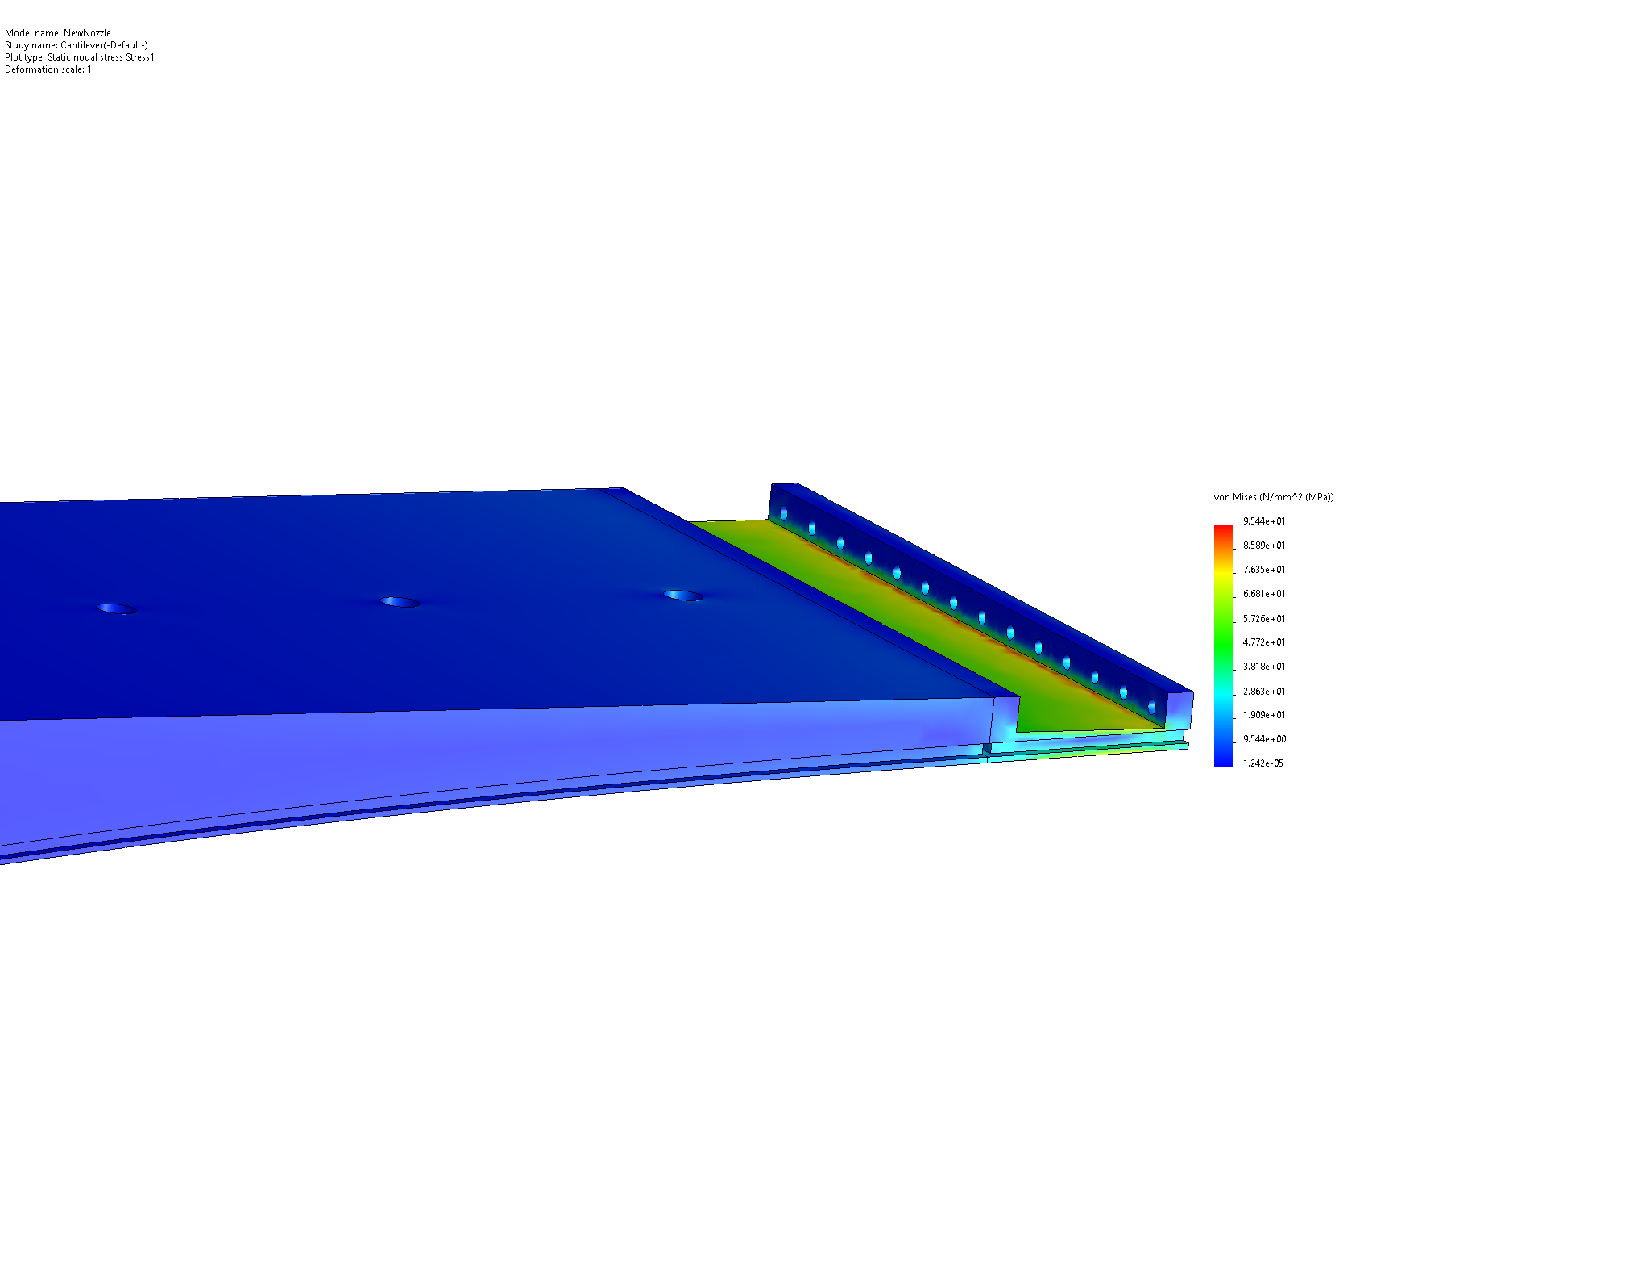
\includegraphics[trim={110 200 180 200},clip,width=4.5in]{fea-flexure.pdf}
    \caption{Flexure stress at maximum deflection of 0.25 inches}
    \label{fig:fea-flexure}
\end{figure}

\section{Fabrication Plans}

At present, all of the ACE2.0 parts are finished machining besides the nozzles and sidewalls. The fabrication is following the schedule shown in Figure \ref{fig:schedule}, which shows the completed tasks in gray, the current tasks in green, orange, or red depending on status, and future tasks in white. The frame pieces were machined at the Texas A\&M Fischer Engineering Design Center (FEDC). An image of the brace after being cut out on the water jet is shown in Figure \ref{fig:fab-brace-jet}. The pallet of finished frame parts is shown in Figure \ref{fig:fab-frame-parts}.

\begin{figure}[ht!]
    \centering
    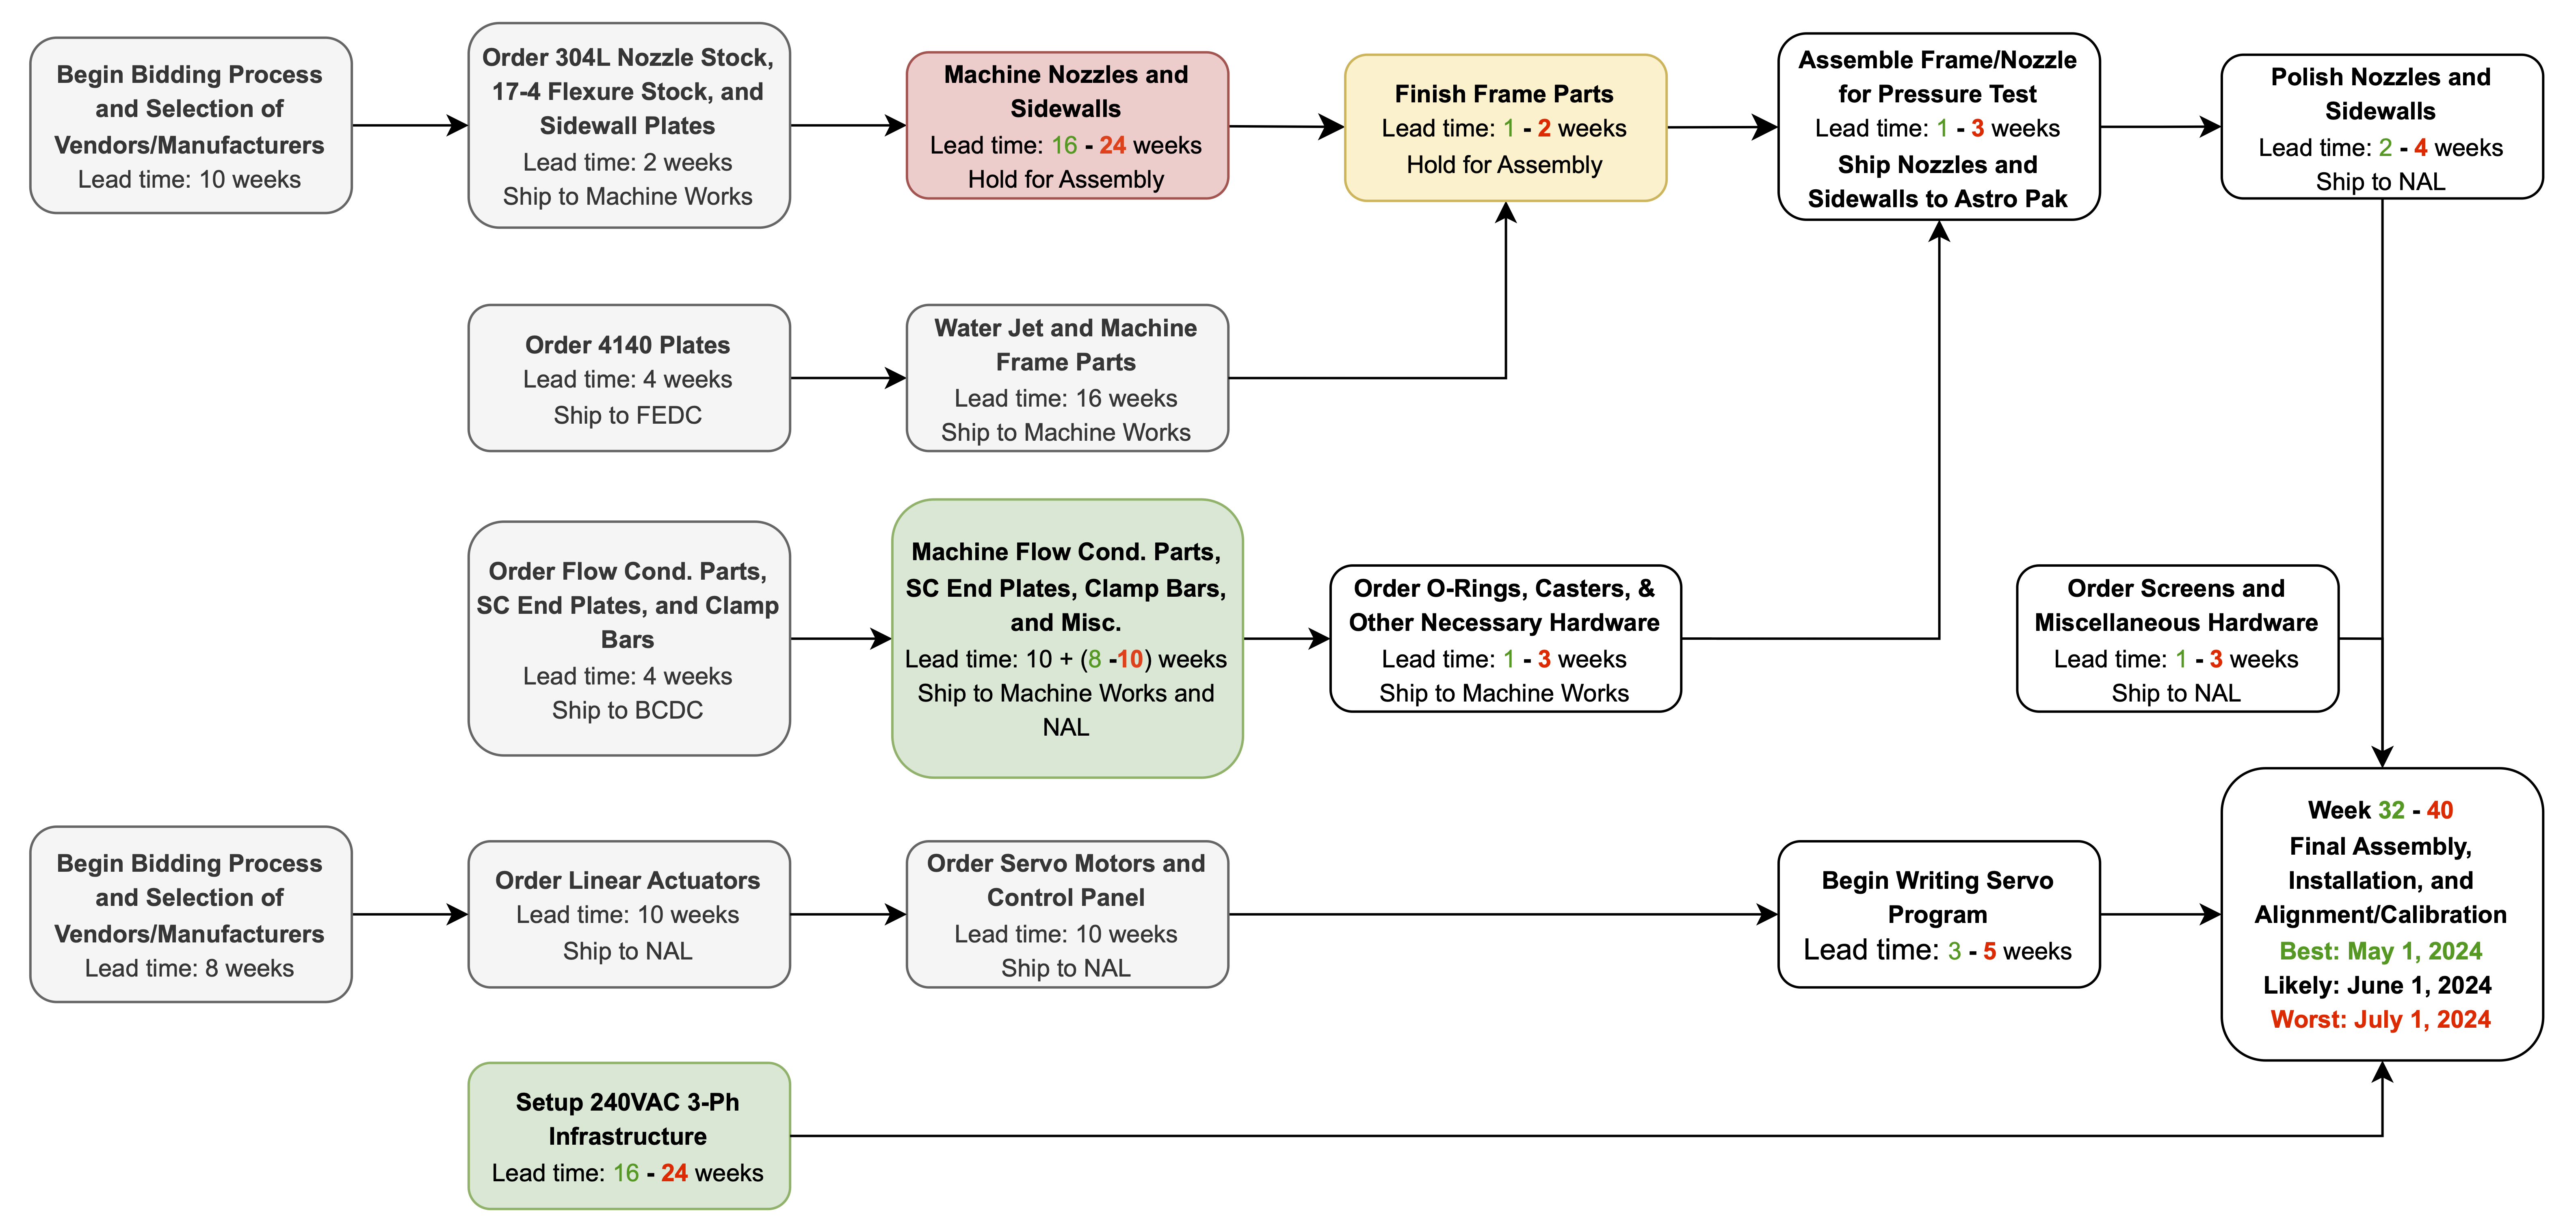
\includegraphics[width=6in]{schedule}
    \caption{Manufacturing schedule beginning from September 25, 2023}
    \label{fig:schedule}
\end{figure}

\begin{figure}[ht!]
    \centering
    \includegraphics[width=5in]{fab-brace-jet}
    \caption{Rough cut brace on water jet}
    \label{fig:fab-brace-jet}
\end{figure}

\begin{figure}[ht!]
    \centering
    \includegraphics[width=5in]{fab-frame-parts}
    \caption{Pallet of finished frame parts from FEDC}
    \label{fig:fab-frame-parts}
\end{figure}

The nozzles and sidewalls are currently being machined at Machine Works Inc. in Bryan, TX. The nozzles were first saw cut to a rough profile to minimize the amount of time on the CNC mill, as shown in Figure \ref{fig:fab-nozzle-saw}. They are currently being machined to a rough contour, and then the back of each will be machined flat prior to finishing the contour. For the final passes, the nozzle blocks and flexures will be bolted together to ensure there is no step between the two pieces. Machine Works will also finish the brace for the frame by drilling and tapping holes.

\begin{figure}[ht!]
    \centering
    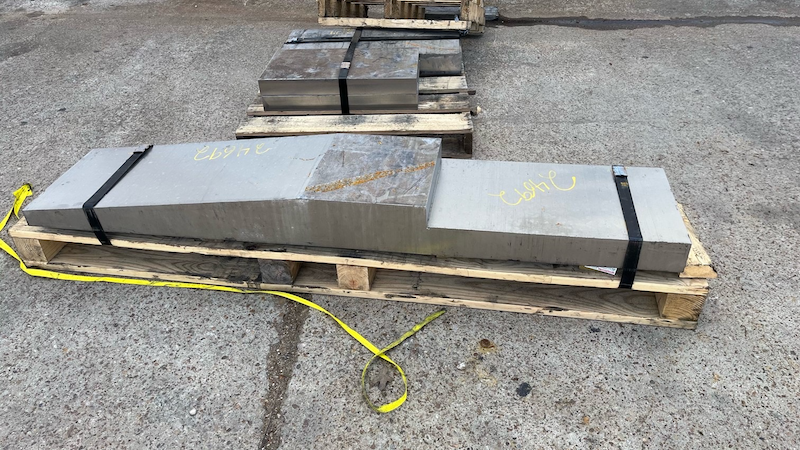
\includegraphics[width=5in]{fab-nozzle-saw}
    \caption{Nozzle block saw cut to rough profile}
    \label{fig:fab-nozzle-saw}
\end{figure}

The rest of the parts were machined at the Texas A\&M Bush Combat Development Complex (BCDC). All of these parts are finished, but only the parts necessary for the pressure test have been picked up. Figures \ref{fig:fab-flow-box}, \ref{fig:fab-aerogrid}, and \ref{fig:fab-cone} show the flow conditioner box, an aerogrid, and a flow spreading cone. BCDC will be the primary machine shop for any future fabrication throughout this work.

\begin{figure}[ht!]
    \centering
    \includegraphics[width=6in]{fab-flow-box}
    \caption{Machined flow conditioner box}
    \label{fig:fab-flow-box}
\end{figure}

\begin{figure}[ht!]
    \centering
    \includegraphics[width=6in]{fab-aerogrid}
    \caption{Machined aerogrid}
    \label{fig:fab-aerogrid}
\end{figure}

\begin{figure}[ht!]
    \centering
    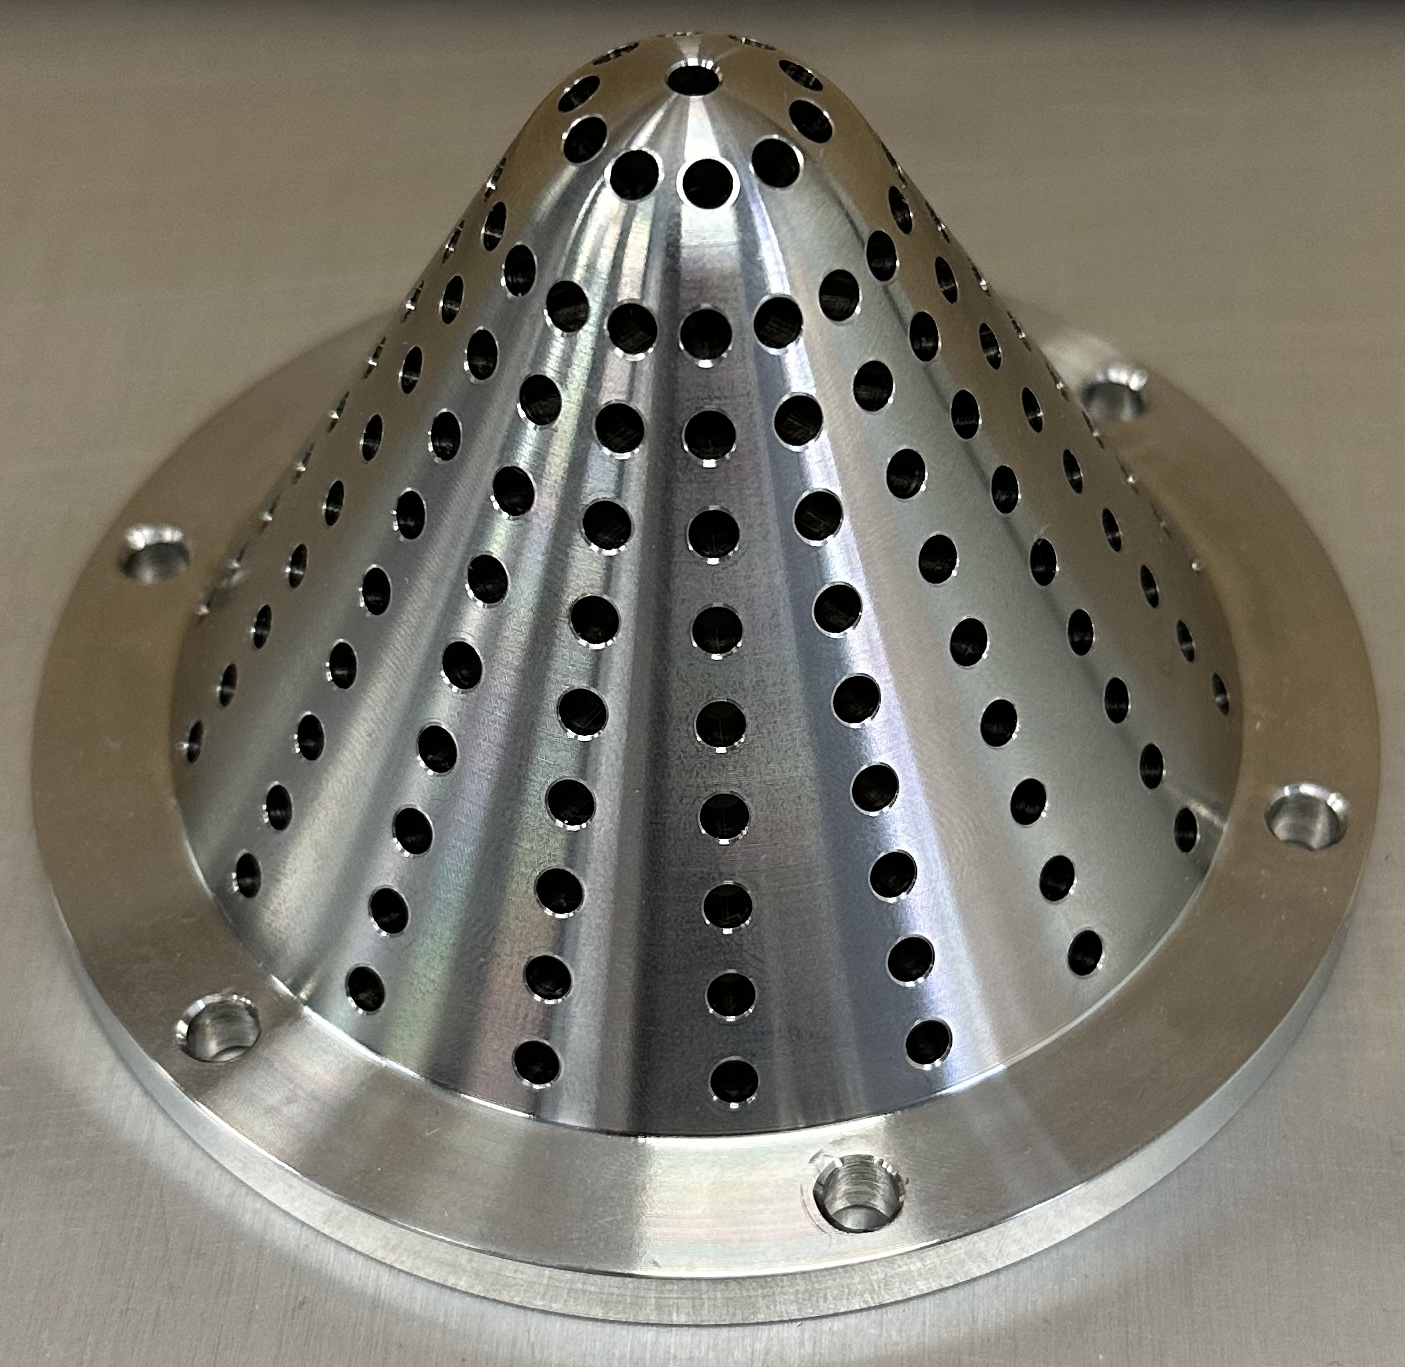
\includegraphics[width=4in]{fab-cone}
    \caption{Machined flow spreading cone}
    \label{fig:fab-cone}
\end{figure}

\clearpage

\subsection{Pressure Test}

The hydro-pressure test will be performed at Machine Works prior to sending the nozzles and sidewalls to be polished. The base tunnel will be assembled with steel bars to simulate the actuators. The tunnel will be filled with water and pressurized to 200 psia for one hour, and the pressure will be monitored throughout. The primary goal of the pressure test is to ensure structural integrity at maximum pressure. Any major leaks will also be addressed.

\subsection{Polishing}

Following the completion of the pressure test, the nozzles and sidewalls will be shipped to Astro Pak for polishing. All interior surfaces will be mechanically polished to a 1 Ra\footnote{Surface roughness average of 1 microinch} finish, and electropolishing will be used if necessary. In order to safely ship these pieces, the nozzle blocks will be assembled as shown in Figure \ref{fig:polish-assembly} and custom wooden crates will be built.

\begin{figure}[ht!]
    \centering
    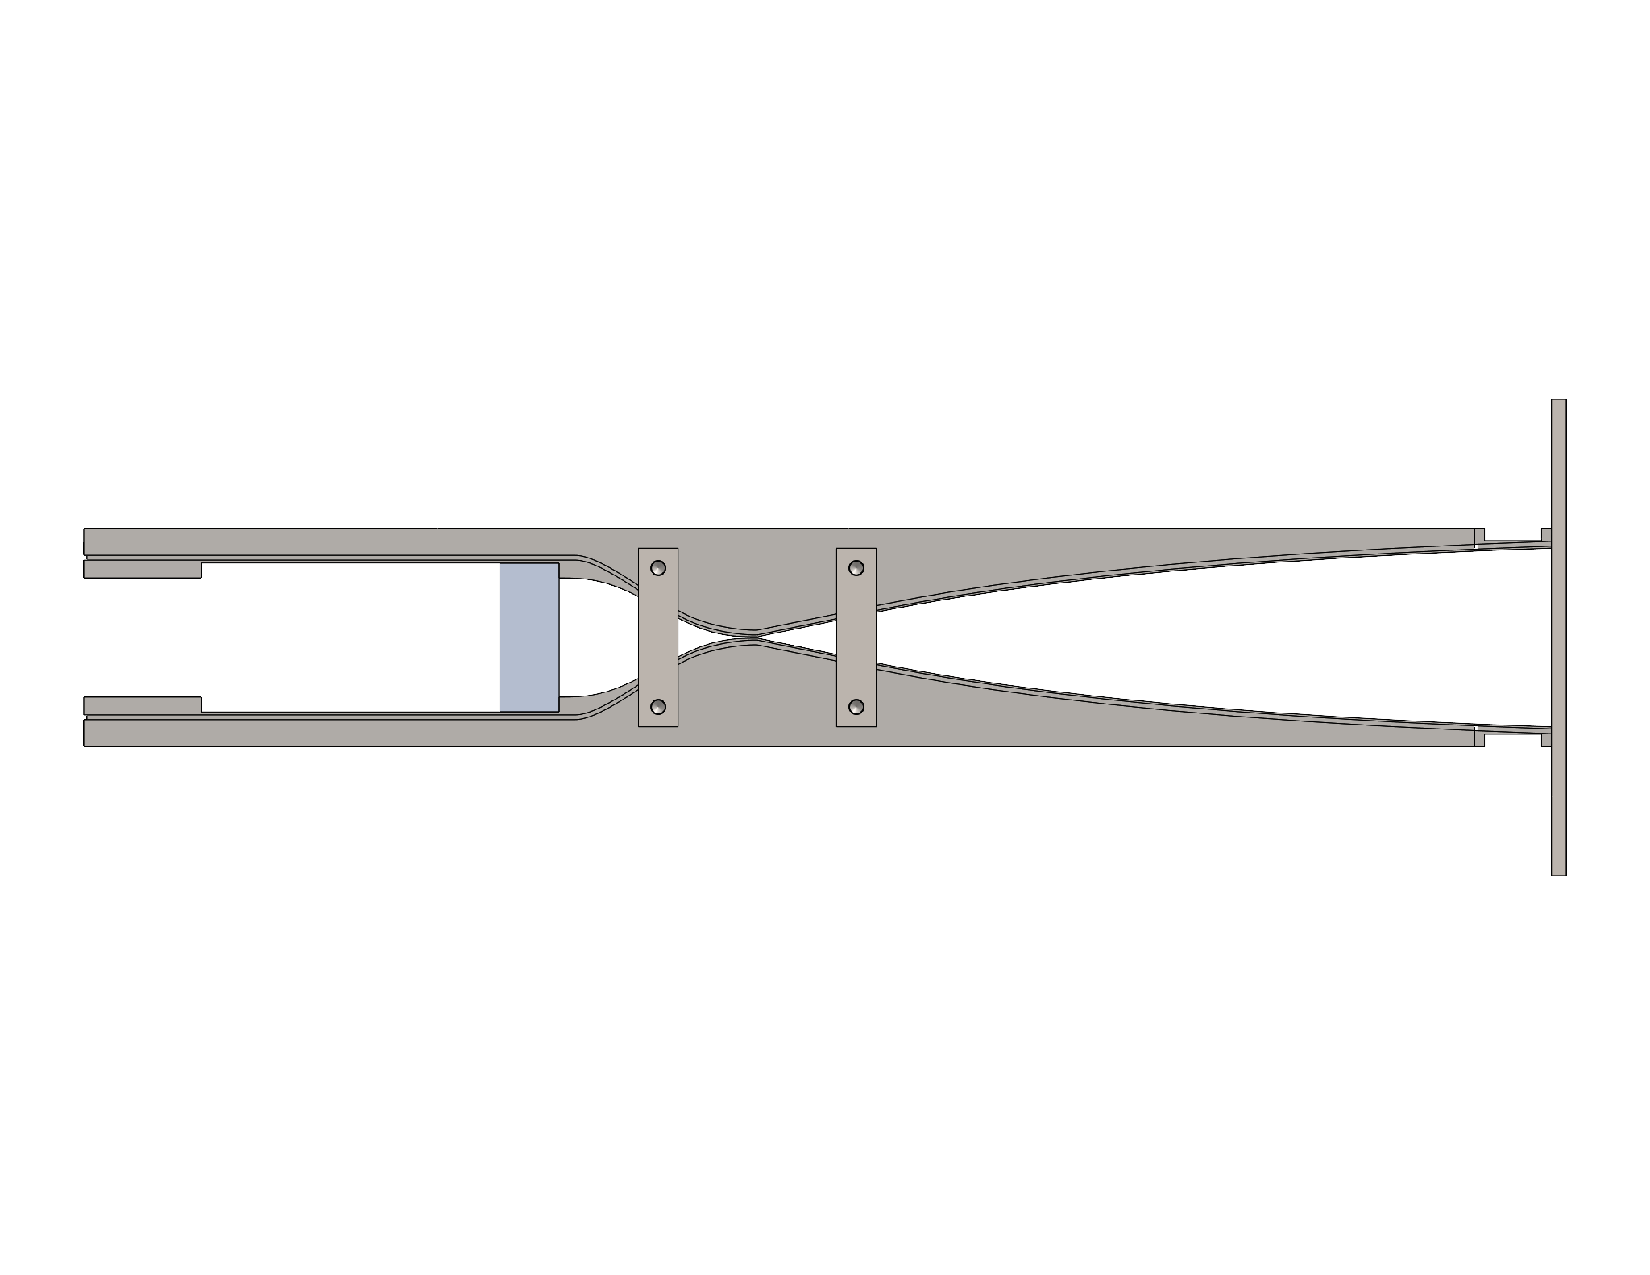
\includegraphics[trim={30 170 30 170},clip,width=5in]{polish-assembly.pdf}
    \caption{Nozzle assembly for shipping to polishing vendor}
    \label{fig:polish-assembly}
\end{figure}

\section{Final Assembly, Installation, and Calibration}

The final assembly will occur at the NAHL once the nozzle and sidewalls are delivered from polishing. Once nozzles and actuators are assembled in the frame, ACE2.0 will be rolled into the lab to replace ACE. All hoses, wires, and instrumentation attached to the nozzle and settling chamber will be removed and ACE will be rolled out of the lab. ACE2.0 will roll in and reconnect all hoses, wires, and instrumentation.

The nozzles will be leveled and aligned and then the servos will homed with the limit switches to calibrate the actuation system. The pressure and temperature instrumentation will be calibrated prior to reconnecting to the new facility. The sidewalls will then be mounted for the shakedown run, which will include a pitot rake at the nozzle exit to ensure uniformity in the test section.

% \subsection{Nozzle Alignment and Actuation Homing}

% \textcolor{red}{How to properly align and level nozzle?}

% Before the sidewalls are installed, the nozzles will be aligned and leveled and then actuated for homing the servo motors with the limit switches. At this point shims will be used to make fine adjustments to limit switch positions to ensure a minimum Mach number of \textcolor{red}{4.9?} and a maximum Mach number of \textcolor{red}{8.5?}.

% \subsection{Shakedown and Calibration}

% \textcolor{red}{Decide what the first runs and measurements should be to properly calibrate following relevant literature.}

